%===============================================================================
% $Id: ifacconf.tex 19 2011-10-27 09:32:13Z jpuente $  
% Template for IFAC meeting papers
% Copyright (c) 2007-2008 International Federation of Automatic Control
%===============================================================================
\documentclass[a4paper]{ifacconf}

\usepackage{graphicx,amsmath,url}      % include this line if your document contains figures
\usepackage[round]{natbib}             % required for bibliography
%===============================================================================


% ===============================================================
% Choose the language of the manuscript.
% If in English, choose 
% \def\portugues{0} 
%
% If in Portuguese or Spanish, choose
% \def\portugues{1} 
%
% Note that, if you are writing in Spanish, you need additional 
% adjusts in some parts of the text, which have been put in Portuguese only.
\def\portugues{1} 
% ===============================================================

% If the above line is commented, it is assumed manuscript in English:
\ifx\portugues\undefined
\def\portugues{0}
\fi


\if\portugues0
   \usepackage[english]{babel}
  \else
   \usepackage[spanish,brazil,english]{babel}
\fi

  

\usepackage[T1]{fontenc}
%\usepackage{inputenc}

\usepackage[utf8]{inputenc}

\usepackage{ae}


\if\portugues1
% =====================================================================
% =====================================================================
% If the manuscript is in Spanish, please change the texts adequatelly.
% You may also add other definitions in this part.
 \newtheorem{teorema}[thm]{{\em Teorema}}{ }
 \newtheorem{lema}[thm]{{\em Lema}}{ }
 \newtheorem{corolario}[thm]{{\em Corolário}}{ }
 \newenvironment{prova}{{\bf Prova.}}{ }
% ===============================================================
\fi

\begin{document}


\if\portugues1

   % =====================================================================
   % =====================================================================
   % USE THIS PART IF THE TEXT IS IN PORTUGUES OR SPANISH
   % =====================================================================
   % If the manuscript is in Spanish, please change the texts adequately.
   % =====================================================================
   % 
   \selectlanguage{brazil}

   \begin{frontmatter}

      \title{Controle Digital de Pressão Hidráulica em Módulo de Frenagem para Aplicações ADAS}
      % Title, preferably not more than 10 words.

      %\thanks[footnoteinfo]{Reconhecimento do suporte financeiro deve vir nesta nota de rodapé.}


      \author[First]{Elton Inacio Alves Junior}
      % \author[Second]{Segundo B. Autor} 
      % \author[Third]{Terceiro C. Autor}

      \address[First]{Departamento de Engenharia de Sistemas Eletrônicos, Universidade De São Paulo - USP.}
      % \address[Second]{Faculdade de Engenharia de Controle \& Automação, Universidade do Futuro, RJ (e-mail: autor2@feca.unifutu.rj)}
      % \address[Third]{Electrical Engineering Department, Seoul National University, Seoul, Korea, (e-mail: author3@snu.ac.kr)}


      \selectlanguage{english}
      \renewcommand{\abstractname}{{\bf Abstract:~}}
      \begin{abstract}                % Abstract of not more than 250 words.
         The integration of longitudinal advanced driver assistance systems (ADAS) functions (e.g., adaptive cruise control (ACC) and automatic emergency braking (AEB)) with the braking system requires a pressure actuator that delivers predictable behavior under physical constraints and model uncertainties of the electro-hydraulic unit. This paper presents a modeling and digital control methodology for wheel brake pressure regulation using an anti-lock braking system/electronic stability control (ABS/ESC) hydraulic modulator operating in active braking mode, where the pressure reference is treated as an external command generated by a higher-level controller. The plant is described by a lumped nonlinear two-pressure hydraulic model (supply and wheel-channel pressures) with pump and orifice-based flow laws. A local linearization around a braking operating point yields a state-space model that is discretized via zero-order hold (ZOH) and used to design a discrete-time LQI controller with integral action, combined with a discrete Luenberger observer. Actuator saturations and a discrete valve logic with hysteresis are included to reflect typical modulator operation. The approach is assessed in MATLAB/Simulink through stepwise pressure tracking tests, performance metrics, and a parametric sensitivity sweep to discuss robustness. Simulation evidence indicates the feasibility of pressure tracking with command signals consistent with actuation limits, supporting future embedded implementation.

         \vskip 1mm% não altere esse espaçamento
         \selectlanguage{brazil}
         {\noindent \bf Resumo}:  A integração de funções de Sistemas Avançados de Assistência ao Condutor (ADAS) para controle longitudinal (por exemplo, Controle de Cruzeiro Adaptativo (ACC) e Frenagem Autônoma de Emergência (AEB)) com o sistema de freio demanda um atuador de pressão capaz de responder com previsibilidade, mesmo sob restrições físicas e incertezas do sistema eletro-hidráulico. Este artigo apresenta uma metodologia de modelagem e controle digital para o regulador de pressão por roda em um módulo hidráulico de sistema antibloqueio de freios e controle eletrônico de estabilidade (ABS/ESC) operando em frenagem ativa, tratando a referência de pressão como um sinal proveniente de um controlador de nível superior. A planta é representada por um modelo hidráulico não linear concentrado em duas pressões (suprimento e canal de roda), com leis de vazão baseadas em bomba e orifício. A partir de uma linearização local em regime de frenagem, obtém-se um modelo em espaço de estados discretizado por retenção de ordem zero (ZOH) para síntese de um controlador LQI em tempo discreto, acoplado a um observador discreto de Luenberger, com saturações e lógica discreta de válvulas (com histerese) compatíveis com a atuação típica do modulador. A abordagem é avaliada em MATLAB/Simulink, com ensaios de seguimento de referência em patamares, análise por métricas de desempenho e varredura de sensibilidade paramétrica para caracterizar robustez. Os resultados em simulação indicam viabilidade do seguimento de pressão com coerência de comandos frente às limitações de atuação, apoiando a continuidade rumo à implementação embarcada.
      \end{abstract}

      \selectlanguage{english}


      \begin{keyword}
         active braking; digital control; hydraulic pressure regulation; LQI; Luenberger observer; ADAS; MATLAB/Simulink.

         \vskip 1mm% não altere esse espaçamento
         \selectlanguage{brazil}
         {\noindent\it Palavras-chaves:} frenagem ativa; controle digital; regulação de pressão hidráulica; LQI; observador de Luenberger; ADAS; MATLAB/Simulink.
      \end{keyword}


      \selectlanguage{brazil}


   \end{frontmatter}
\else
   % ===============================================================
   % ===============================================================
   % USE THIS PART IF THE TEXT IS IN ENGLISH
   % ===============================================================
   % ===============================================================
   % 

   \begin{frontmatter}

      \title{Style for SBA Conferences \& Symposia: Use Title Case for
         Paper Title\thanksref{footnoteinfo}}
      % Title, preferably not more than 10 words.

      \thanks[footnoteinfo]{Sponsor and financial support acknowledgment
         goes here. Paper titles should be written in uppercase and lowercase
         letters, not all uppercase.}

      \author[First]{First A. Author}
      \author[Second]{Second B. Author, Jr.}
      \author[Third]{Third C. Author}


      \address[First]{Faculdade de Engenharia Elétrica, Universidade do Triângulo, MG, (e-mail: autor1@faceg@univt.br).}
      \address[Second]{Faculdade de Engenharia de Controle \& Automação, Universidade do Futuro, RJ (e-mail: autor2@feca.unifutu.rj)}
      \address[Third]{Electrical Engineering Department,
         Seoul National University, Seoul, Korea, (e-mail: author3@snu.ac.kr)}

      \renewcommand{\abstractname}{{\bf Abstract:~}}

      \begin{abstract}                % Abstract of not more than 250 words.
         These instructions give you guidelines for preparing papers for IFAC
         technical meetings. Please use this document as a template to prepare
         your manuscript. For submission guidelines, follow instructions on
         paper submission system as well as the event website.
      \end{abstract}

      \begin{keyword}
         Five to ten keywords, preferably chosen from the IFAC keyword list.
      \end{keyword}

   \end{frontmatter}
\fi

%===============================================================================
%===============================================================================
%===============================================================================


\section{Introdução}

A frenagem automotiva permanece no centro das discussões sobre segurança veicular porque concentra, em um mesmo momento, decisões humanas, limitações físicas do pneu--pista e restrições do sistema atuador. Além de desacelerar o veículo até a parada, o sistema de freio precisa operar com previsibilidade em diferentes condições de carga, aderência e temperatura, preservando dirigibilidade e estabilidade \cite{Rudolf2011,Konrad2014}. Esse requisito torna-se ainda mais explícito quando a demanda de frenagem deixa de ser exclusivamente comandada pelo condutor e passa a ser executada por funções de assistência à condução.

Sistemas Avançados de Assistência ao Condutor (ADAS) utilizam sensores e algoritmos para apoiar o controle longitudinal e lateral do veículo, o que inclui funções como Controle de Cruzeiro Adaptativo (ACC) e Frenagem Autônoma de Emergência (AEB) \cite{Lentin2022}. Nesses casos, a cadeia de controle tende a ser hierárquica: um módulo de alto nível opera uma desaceleração desejada (ou uma demanda equivalente de torque/força) e, a jusante, o sistema de frenagem deve converter essa solicitação em pressão hidráulica efetiva nas rodas. A qualidade dessa conversão não é um detalhe de implementação; ela influencia diretamente o conforto, a repetibilidade e a robustez do comportamento longitudinal, especialmente quando o veículo opera próximo a limites de atuação ou quando há incertezas e ruídos de medição.

Nas arquiteturas atuais, o conjunto eletro-hidráulico associado às unidades de sistema antibloqueio de freios e controle eletrônico de estabilidade (ABS/ESC) -- bomba, válvulas e eletrônica -- pode atuar não apenas como modulador durante eventos de escorregamento, mas também como fonte/atuador de pressão em cenários de frenagem ativa. Do ponto de vista de modelagem e projeto de controle, isso traz um desafio concreto: a dinâmica hidráulica é intrinsecamente não linear, dependente de diferenças de pressão e de restrições de vazão, e a atuação é limitada por saturações físicas e pela natureza discreta de válvulas solenóides (tipicamente operando em estados aberto/fechado). Trabalhos recentes exploram tanto modelos concentrados e aplicações experimentais em unidades hidráulicas \cite{HouhuaJing2022,ZengYangHuang2023} quanto estratégias de coordenação e modulação de pressão \cite{Lv2014,ChenLv2017,PressureCoordinatedControl2023}. Ainda assim, ao observar uma implementação embarcada realista, permanece a necessidade de um fluxo de projeto que conecte, de forma rastreável, (i) um modelo hidráulico suficientemente simples para síntese, (ii) um regulador digital em tempo discreto, e (iii) um conjunto explícito de restrições de atuação e hipóteses de operação compatíveis com o uso do módulo ABS/ESC como atuador de frenagem ativa.

Este artigo aborda esse recorte: controle digital de pressão hidráulica por roda (baixo nível), com referência proveniente de um controlador longitudinal de nível superior. A contribuição não é propor um novo paradigma de controle para frenagem, mas consolidar um encadeamento metodológico adequado à transição de \textit{model-in-the-loop} para etapas futuras de implementação embarcada e validação em bancada, alinhado a práticas de verificação orientadas por simulação em sistemas de controle embarcados \cite{KapinskiJamesDeshmukh2016}.

O objetivo do trabalho é projetar e avaliar, em simulação, uma estratégia de seguimento de referência de pressão por roda utilizando o módulo hidráulico (ABS/ESC) como atuador, considerando não linearidades hidráulicas e limitações físicas de atuação. Para isso, emprega-se um modelo hidráulico não linear concentrado em duas pressões (suprimento e canal de roda), linearização local em torno de um ponto de operação de frenagem e síntese de um controlador discreto em espaço de estados do tipo LQI, acoplado a um observador de Luenberger em tempo discreto. As restrições de atuação (saturações) e a lógica discreta de válvulas são incorporadas para manter coerência com o funcionamento esperado do modulador. A avaliação em MATLAB/Simulink utiliza ensaios de seguimento de referência e análise de sensibilidade paramétrica, de modo a organizar a discussão em termos de desempenho e esforço de atuação, sem extrapolar para conclusões experimentais fora do escopo simulado.

O artigo está organizado da seguinte forma: a Seção~\ref{sec:modelagem} descreve o modelo hidráulico e as hipóteses de atuação; a Seção~\ref{sec:controle} apresenta a linearização, discretização e o projeto do regulador LQI e do observador; a Seção~\ref{sec:simulacao} apresenta os cenários de simulação e os critérios de avaliação; por fim, a Seção~\ref{sec:resultados} discute os resultados e aponta continuidades naturais, incluindo a implementação embarcada e a validação em bancada.

\section{Modelagem do atuador eletro-hidráulico e hipóteses de atuação}
\label{sec:modelagem}
Esta seção descreve a planta considerada no artigo e apresenta as hipóteses adotadas para que o problema de controle seja bem delimitado. O recorte assume o módulo eletro-hidráulico associado a unidades ABS/ESC como atuador de pressão em frenagem ativa, isto é, capaz de gerar e modular pressão no canal de roda a partir de comandos elétricos de bomba e válvulas. A descrição física e funcional desses módulos pode ser encontrada em referências clássicas de sistemas de freio e assistência ao condutor \cite{Konrad2014,Rudolf2011} e em trabalhos recentes voltados a controle/validação de unidades hidráulicas \cite{HouhuaJing2022,ZengYangHuang2023}.

\subsection{Da desaceleração à referência de pressão (sinal externo ao regulador)}
Para integrar o regulador de pressão com uma função longitudinal de nível superior (por exemplo, ACC/AEB), é natural que o controlador superior forneça uma demanda em termos de desaceleração desejada. Como este artigo não tem por objetivo validar um modelo completo de veículo, pneu e sistema de freio, adota-se um mapeamento agregador simples para gerar referências de pressão com ordem de grandeza compatível com os ensaios. Assim, a referência por roda é tratada como entrada do problema de controle e pode ser definida por:
\begin{equation}
   P_{\mathrm{ref}}(t) = \frac{m}{A_c}\,\max\big(-a_{\mathrm{ego}}(t),\,0\big),
   \label{eq:aref_to_pref}
\end{equation}
em que $m$ representa a massa equivalente do veículo e $A_c$ agrega, em um único ganho, efeitos de repartição, conversão pressão--força e eficiência do conjunto de freio. O uso desse mapeamento tem um propósito metodológico: isolar a dinâmica do atuador hidráulico sob controle e discutir desempenho e restrições sem confundir o resultado com a qualidade de um modelo longitudinal completo \cite{Lentin2022}.

\subsection{Modelo hidráulico não linear concentrado (duas pressões)}
A planta é modelada por uma representação concentrada em duas regiões compressíveis: a pressão de suprimento/manifold $P_{sup}$ e a pressão no canal de roda $P_w$, em linha com abordagens comuns na literatura para projeto e validação \cite{HouhuaJing2022,Lv2014,ZengYangHuang2023}. O vetor de estados e o vetor de comandos são definidos como:
\begin{equation}
   x(t)=\begin{bmatrix} P_{sup}(t) \\ P_w(t) \end{bmatrix},
   \qquad
   u(t)=\begin{bmatrix} \omega_p(t) \\ u_{in}(t) \\ u_{out}(t) \end{bmatrix},
   \label{eq:states_inputs}
\end{equation}
em que $\omega_p$ é a velocidade da bomba e $u_{in}$ e $u_{out}$ representam os comandos associados às válvulas de entrada e saída. Neste trabalho, tais comandos são binários (válvula fechada/aberta), isto é, $u_{in},u_{out}\in\{0,1\}$.

A dinâmica de pressão decorre da continuidade para fluido compressível:
\begin{equation}
   \dot{P}_{sup} = \frac{\beta}{V_{sup}}\big(Q_{pump}-Q_{in}-Q_{\mathrm{leak},sup}\big),
   \label{eq:pressure_sup}
\end{equation}

\begin{equation}
   \dot{P}_{w} = \frac{\beta}{V_{w}}\big(Q_{in}-Q_{out}-Q_{\mathrm{leak},w}\big),
   \label{eq:pressure_wheel}
\end{equation}
onde $\beta$ é o módulo volumétrico efetivo e $V_{sup}$ e $V_w$ são volumes equivalentes.

A vazão da bomba é modelada por relação afim com $\omega_p$ e termo de vazamento interno (para o retorno), conforme modelos frequentemente adotados em estudos eletro-hidráulicos \cite{MotorParametricDesign2023,WangBingbing2015}:
\begin{equation}
   Q_{pump} = K_b\,\omega_p - K_{lb}\big(P_{sup}-P_{ret}\big).
   \label{eq:qpump}
\end{equation}

Em particular, $P_{ret}$ é a pressão do retorno/reservatório, tratada como aproximadamente constante nos ensaios e no modelo.

As vazões nas válvulas são descritas por lei de orifício (Torricelli/Bernoulli), com coeficiente de descarga, adotando o operador $(\cdot)_+=\max(\cdot,0)$ para impedir raiz de argumento negativo:
\begin{equation}
   Q_{in} = C_{d,in}\,A_{in}(u_{in})\sqrt{\frac{2\big(P_{sup}-P_w\big)_+}{\rho}},
   \label{eq:qin}
\end{equation}
\begin{equation}
   Q_{out} = C_{d,out}\,A_{out}(u_{out})\sqrt{\frac{2\big(P_{w}-P_{ret}\big)_+}{\rho}},
   \label{eq:qout}
\end{equation}
com $A_{in}(u_{in})=A_{in,\max}u_{in}$ e $A_{out}(u_{out})=A_{out,\max}u_{out}$, e $u_{in},u_{out}\in\{0,1\}$ \cite{ChenLv2017,ProportionalPressureABS2023,Lv2014}. Vazamentos internos podem ser representados por termos proporcionais ao diferencial de pressão, como aproximação de primeira ordem.

A Figura~\ref{fig:modulo_2P_malha_aberta} apresenta um diagrama esquemático do circuito hidráulico considerado, com as variáveis de interesse e os principais componentes destacados.

\IfFileExists{modulo_2P_malha_aberta.png}{%
   \begin{figure}
      \begin{center}
         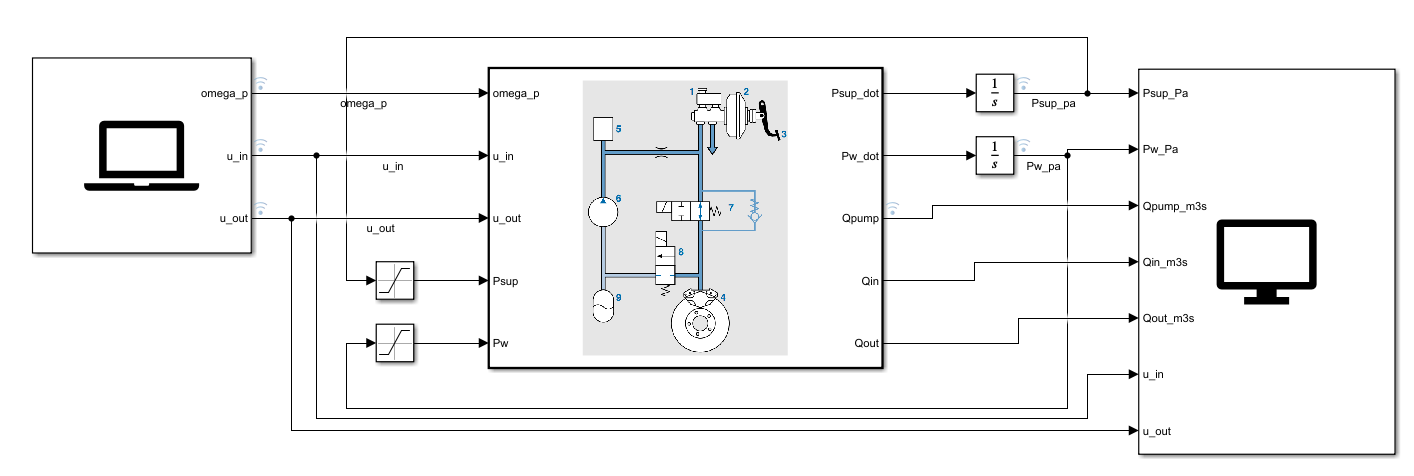
\includegraphics[width=8.4cm]{modulo_2P_malha_aberta.png}
         \caption{Diagrama esquemático do circuito hidráulico considerado, com as variáveis de interesse e os principais componentes destacados.}
         \label{fig:modulo_2P_malha_aberta}
      \end{center}
   \end{figure}}


\subsection{Hipóteses de atuação e restrições}
O foco é o seguimento de referência de $P_w$ sob restrições físicas típicas do atuador: limites de $\omega_p$, de abertura efetiva das válvulas e faixa plausível de pressão. Além disso, por se tratar de um sistema sujeito a instrumentação limitada e incertezas de medição, considera-se a estimação de estados como parte da arquitetura de controle, uma vez que torna o controle mais preciso e robusto.

Nos ensaios, adotam-se limites de atuação coerentes com um modulador ABS/ESC em frenagem ativa, em particular $P_{sup,\max}=100\,\mathrm{bar}$ e $\omega_{p,\max}=100\,\mathrm{rad/s}$, além de comandos discretos $u_{in},u_{out}\in\{0,1\}$.

\section{Projeto do regulador digital em tempo discreto}
\label{sec:controle}
A estratégia de controle proposta combina: (i) um regulador em espaço de estados para a variável contínua $\omega_p$ e (ii) uma lógica discreta para $u_{in}$ e $u_{out}$, de modo a refletir a natureza de atuação do modulador em arquiteturas convencionais. A síntese é feita em tempo discreto para preservar coerência com implementação embarcada \cite{FranklinPowellWorkman1998,Ogata1997}.

\subsection{Linearização local e discretização}
Como a planta \eqref{eq:pressure_sup}--\eqref{eq:qout} é não linear (principalmente pela dependência em $\sqrt{\Delta P}$), adota-se uma linearização local em torno de um ponto de operação de frenagem $(x_0,u_0)$ que satisfaça $P_{sup,0}>P_{w,0}>P_{ret}$ e diferenciais de pressão positivos nas válvulas. A partir disso, obtém-se um modelo linear incremental no formato:
\begin{equation}
   \delta \dot{x}(t)=A\,\delta x(t)+B\,\delta u(t),
   \qquad
   \delta y(t)=C\,\delta x(t),
   \label{eq:lin_ss}
\end{equation}
com $y(t)=P_w(t)$ como variável controlada. Para síntese digital, o modelo é discretizado com retenção de ordem zero (ZOH), resultando em $(A_d,B_d,C_d)$.

\subsection{Controlador LQI e tratamento de saturações}
Para garantir erro estacionário nulo no seguimento de patamares de referência, incorpora-se ação integral sobre o erro $e(k)=P_{\mathrm{ref}}(k)-P_w(k)$, obtendo uma formulação LQI. Em termos conceituais, o regulador resolve um problema de minimização quadrática em tempo discreto e gera a lei de controle:
\begin{equation}
   \omega_p(k) = \mathrm{sat}\big(\omega_{p,\min},\omega_{p,\max},\; -K_x\,\hat{x}(k)-K_i\,x_i(k)\big),
   \label{eq:lqi_control}
\end{equation}
em que $x_i$ é o estado integrador e $\hat{x}$ é o estado estimado. A saturação é explicitada para manter coerência com limites de atuação e evitar comandos inviáveis. Para reduzir risco de \textit{windup} do integrador sob saturação, emprega-se uma estratégia de anti-\textit{windup} compatível com implementação discreta \cite{FranklinPowellWorkman1998,Ogata1997}.

\subsection{Observador discreto de Luenberger}
Como o modelo possui mais estados do que medições diretas, utiliza-se um observador discreto de Luenberger para reconstruir estados necessários à lei de controle:
\begin{equation}
   \hat{x}(k+1)=A_d\hat{x}(k)+B_d u(k)+L\big(y(k)-C_d\hat{x}(k)\big),
   \label{eq:luenberger}
\end{equation}
onde $L$ é escolhido para garantir dinâmica de estimação suficientemente rápida e robusta ao ruído de medição, dentro das limitações do período de amostragem.

\subsection{Lógica discreta para válvulas}
As válvulas são comandadas por uma lógica simples baseada no erro de seguimento, com histerese para evitar comutação excessiva na presença de ruído e discretização:
\begin{itemize}
   \item se $e(k)>\varepsilon$: prioriza-se pressurização ($u_{in}=1$, $u_{out}=0$);
   \item se $e(k)<-\varepsilon$: prioriza-se alívio ($u_{in}=0$, $u_{out}=1$);
   \item se $|e(k)|\le \varepsilon$: aplica-se retenção (\textit{hold}) ($u_{in}=0$, $u_{out}=0$).
\end{itemize}
Esse arranjo busca representar, de modo controlável, os três modos clássicos do canal hidráulico (pressurizar, reter, aliviar) \cite{Konrad2014}, sem assumir válvulas plenamente proporcionais.

\section{Cenários de simulação e critérios de avaliação}
\label{sec:simulacao}
A avaliação em simulação considera ensaios em malha aberta e em malha fechada. A malha aberta tem caráter de verificação de plausibilidade do modelo e exercita os três modos típicos do canal hidráulico (pressurizar, reter e aliviar). A malha fechada permite discutir seguimento de referência e esforço de atuação sob saturações. Para facilitar a leitura, as pressões são apresentadas em $\mathrm{bar}$ nas figuras.

Para discutir sensibilidade a ruído de medição, considera-se o caso em que a pressão medida e disponibilizada ao observador é modelada por:
\begin{equation}
   y(k)=P_w(k)+n(k),
   \label{eq:meas_noise_model}
\end{equation}
onde $n(k)$ é um ruído branco de média zero. No modelo, $P_w$ permanece como a pressão ``verdadeira'' do canal de roda, enquanto $y(k)$ é o sinal usado pelo observador \eqref{eq:luenberger} e, por consequência, pela lei de controle.

A discussão é apoiada em métricas usuais de desempenho, tais como erro RMS, sobressinal, tempos característicos (subida/acomodação), erro estacionário e esforços máximos de controle. Além disso, a robustez é discutida por meio de variação paramétrica em torno do caso nominal, observando-se a degradação de desempenho sob variações de parâmetros físicos (por exemplo, volumes equivalentes, módulo volumétrico efetivo e coeficientes associados à bomba e às válvulas), abordagem alinhada ao uso de simulação como etapa de verificação em sistemas de controle embarcados \cite{KapinskiJamesDeshmukh2016}.

A Figura~\ref{fig:modulo_2P_malha_fechada} apresenta o modelo Simulink utilizado para os ensaios, com os blocos de planta, controlador e lógica de válvulas destacados. O modelo inclui a possibilidade de adicionar ruído de medição e variação paramétrica para análise de sensibilidade.

\IfFileExists{modulo_2P_malha_fechada.png}{%
   \begin{figure}
      \begin{center}
         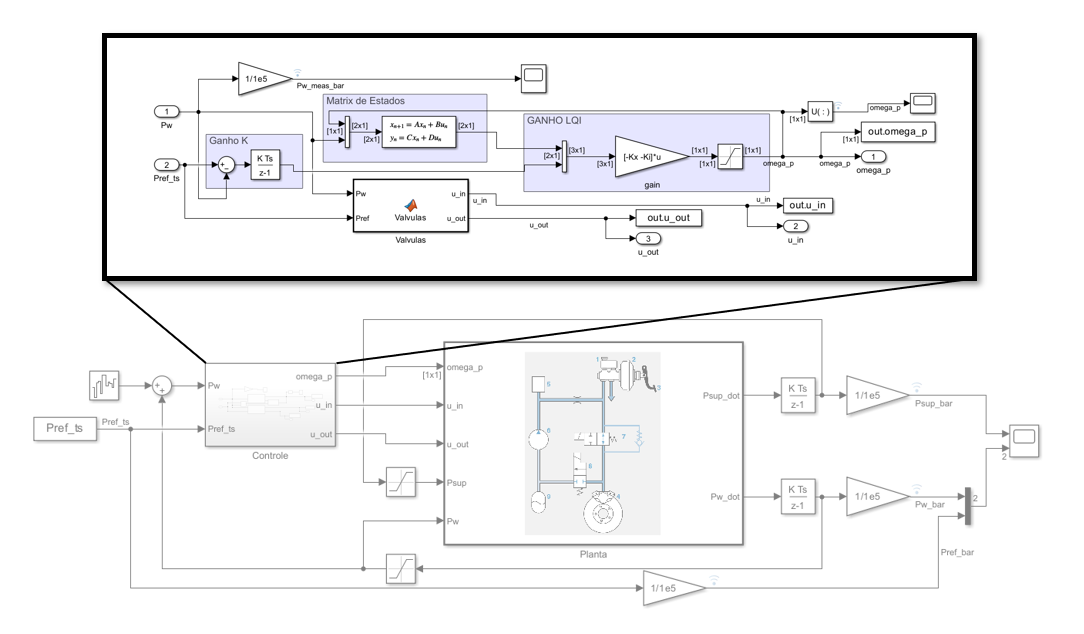
\includegraphics[width=8.4cm]{modulo_2P_malha_fechada.png}
         \caption{Modelo Simulink utilizado para os ensaios, com os blocos de planta, controlador e lógica de válvulas destacados. O modelo inclui a possibilidade de adicionar ruído de medição e variação paramétrica para análise de sensibilidade.}
         \label{fig:modulo_2P_malha_fechada}
      \end{center}
   \end{figure}}



\section{Resultados e discussão}
\label{sec:resultados}
Esta seção organiza os resultados em dois blocos: (i) verificação em malha aberta, para checar coerência causal e ordem de grandeza da planta não linear; e (ii) ensaios em malha fechada, para discutir seguimento de referência de $P_w$, saturações e a sensibilidade do regulador à instrumentação (ruído de medição).

Por consistência com as figuras, as pressões são apresentadas em $\mathrm{bar}$ e interpretadas em relação ao retorno $P_{ret}$. Assim, quando conveniente, utiliza-se a conversão:
\begin{equation}
   P_g = \frac{P-P_{ret}}{10^5},
   \label{eq:pg_def}
\end{equation}
onde $P$ e $P_{ret}$ estão em Pa.

Os ensaios em malha aberta (Figura~\ref{fig:artigo_ensaio_malha_aberta_integrado_real}) confirmam a coerência causal do modelo: na fase de pressurização, a bomba eleva $P_{sup}$ e, quando $P_{sup}>P_w$, estabelece-se vazão positiva na válvula de entrada e aumento de $P_w$; na retenção, com comandos nulos, o comportamento tende a estabilizar; no alívio, a abertura da válvula de saída promove redução de $P_w$ e fluxo para o retorno. Esse resultado é importante porque evita que inconsistências básicas de modelagem dominem a interpretação do controle \cite{HouhuaJing2022,ZengYangHuang2023}.

\begin{figure}
   \begin{center}
      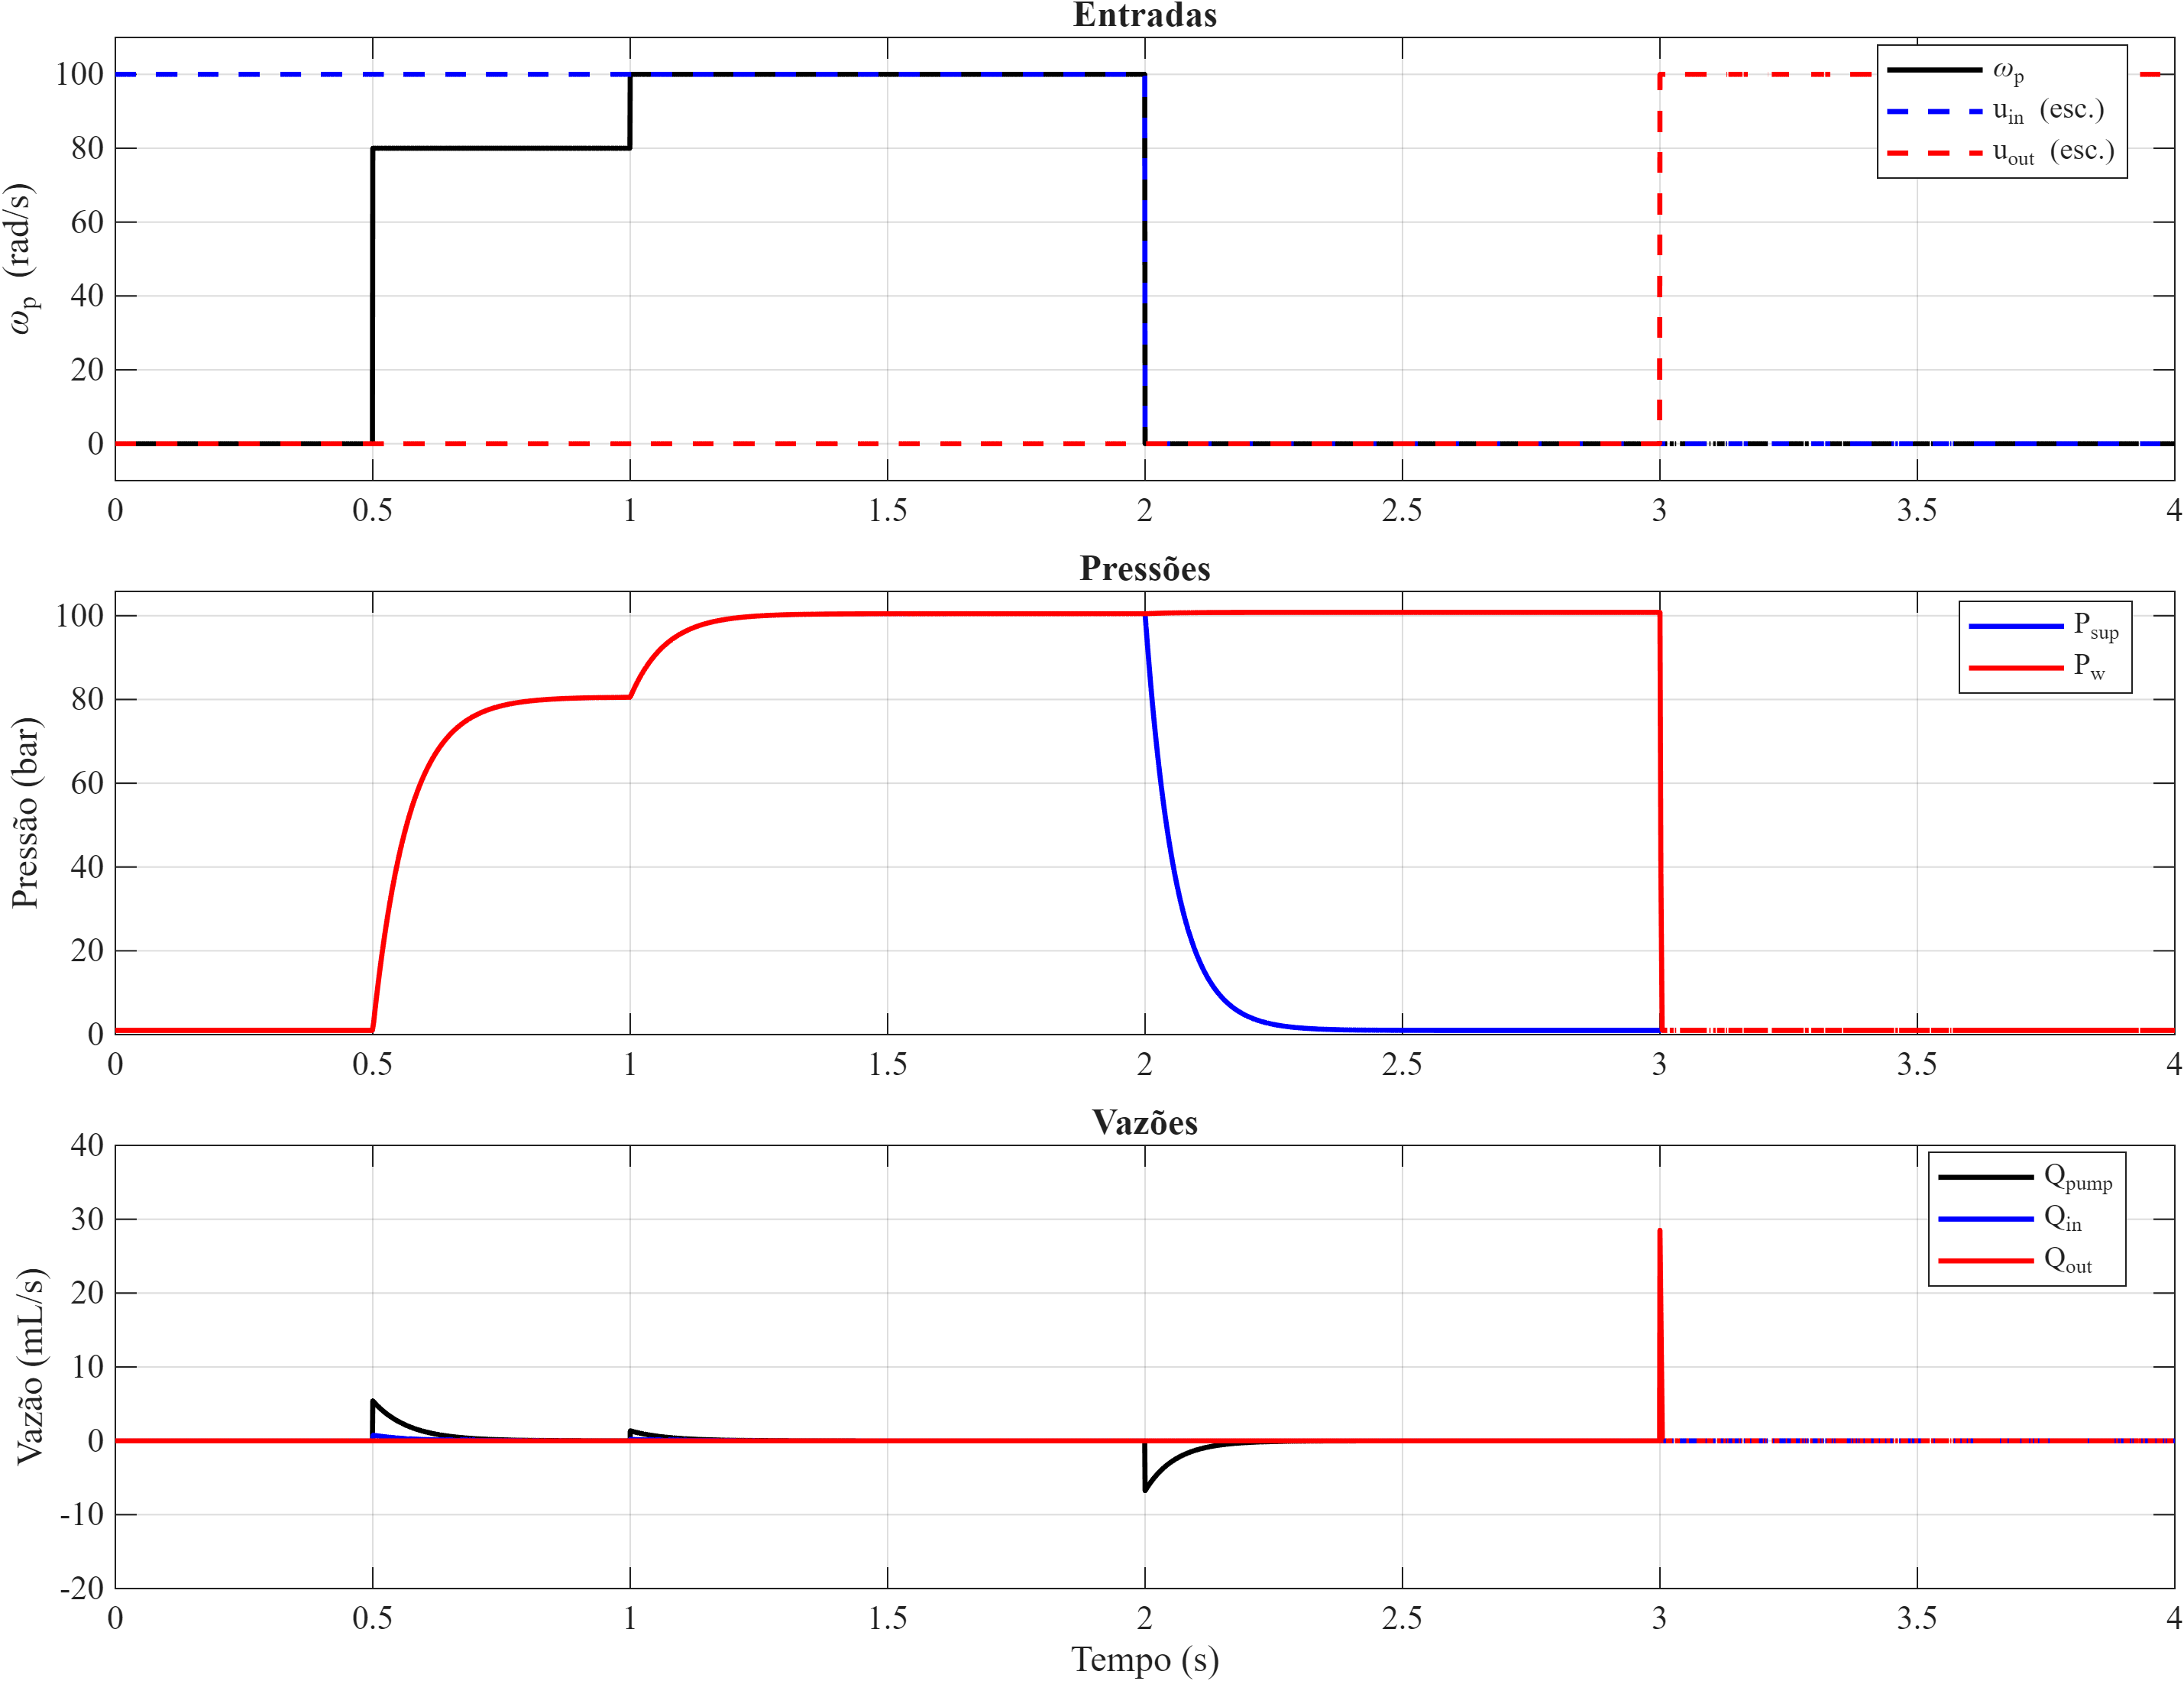
\includegraphics[width=8.4cm]{artigo_ensaio_malha_aberta_integrado_real.png}    % The printed column width is 8.4 cm.
      \caption{Ensaio em malha aberta (três fases).}
      \label{fig:artigo_ensaio_malha_aberta_integrado_real}
   \end{center}
\end{figure}

Em malha fechada (Figura~\ref{fig:simulacao_comandos_e_pressao}), a arquitetura LQI+observador rastreia referências em patamares no modelo não linear com comandos compatíveis com as restrições impostas a $\omega_p$, $u_{in}$ e $u_{out}$. A leitura conjunta de pressão e comandos permite verificar se o seguimento ocorre sem exigir atuações inviáveis e se a lógica discreta de válvulas reproduz os modos de pressurização/retenção/alívio previstos.

Observa-se, ainda, que a não linearidade associada às leis de vazão (dependentes de $\Delta P$) pode introduzir assimetrias entre pressurização e alívio, o que reforça a relevância de explicitar saturações e lógica de válvulas no ensaio, em vez de avaliar apenas um modelo linear idealizado \cite{Lv2014,ChenLv2017}. Nesse contexto, métricas como erro RMS, sobressinal e tempos característicos (subida/acomodação), em conjunto com esforços máximos e indicadores de comutação de válvulas, são naturais para organizar a comparação entre configurações e regimes.



\begin{figure}
   \begin{center}
      
\includegraphics[width=8.4cm]{simulacao_comandos_e_pressao.png}    % The printed column width is 8.4 cm.
      \caption{Simulação em malha fechada: pressão e comandos de atuação.}
      \label{fig:simulacao_comandos_e_pressao}
   \end{center}
\end{figure}

\IfFileExists{artigo_item01_metricas_tracking.png}{%
   \begin{figure}
      \begin{center}
         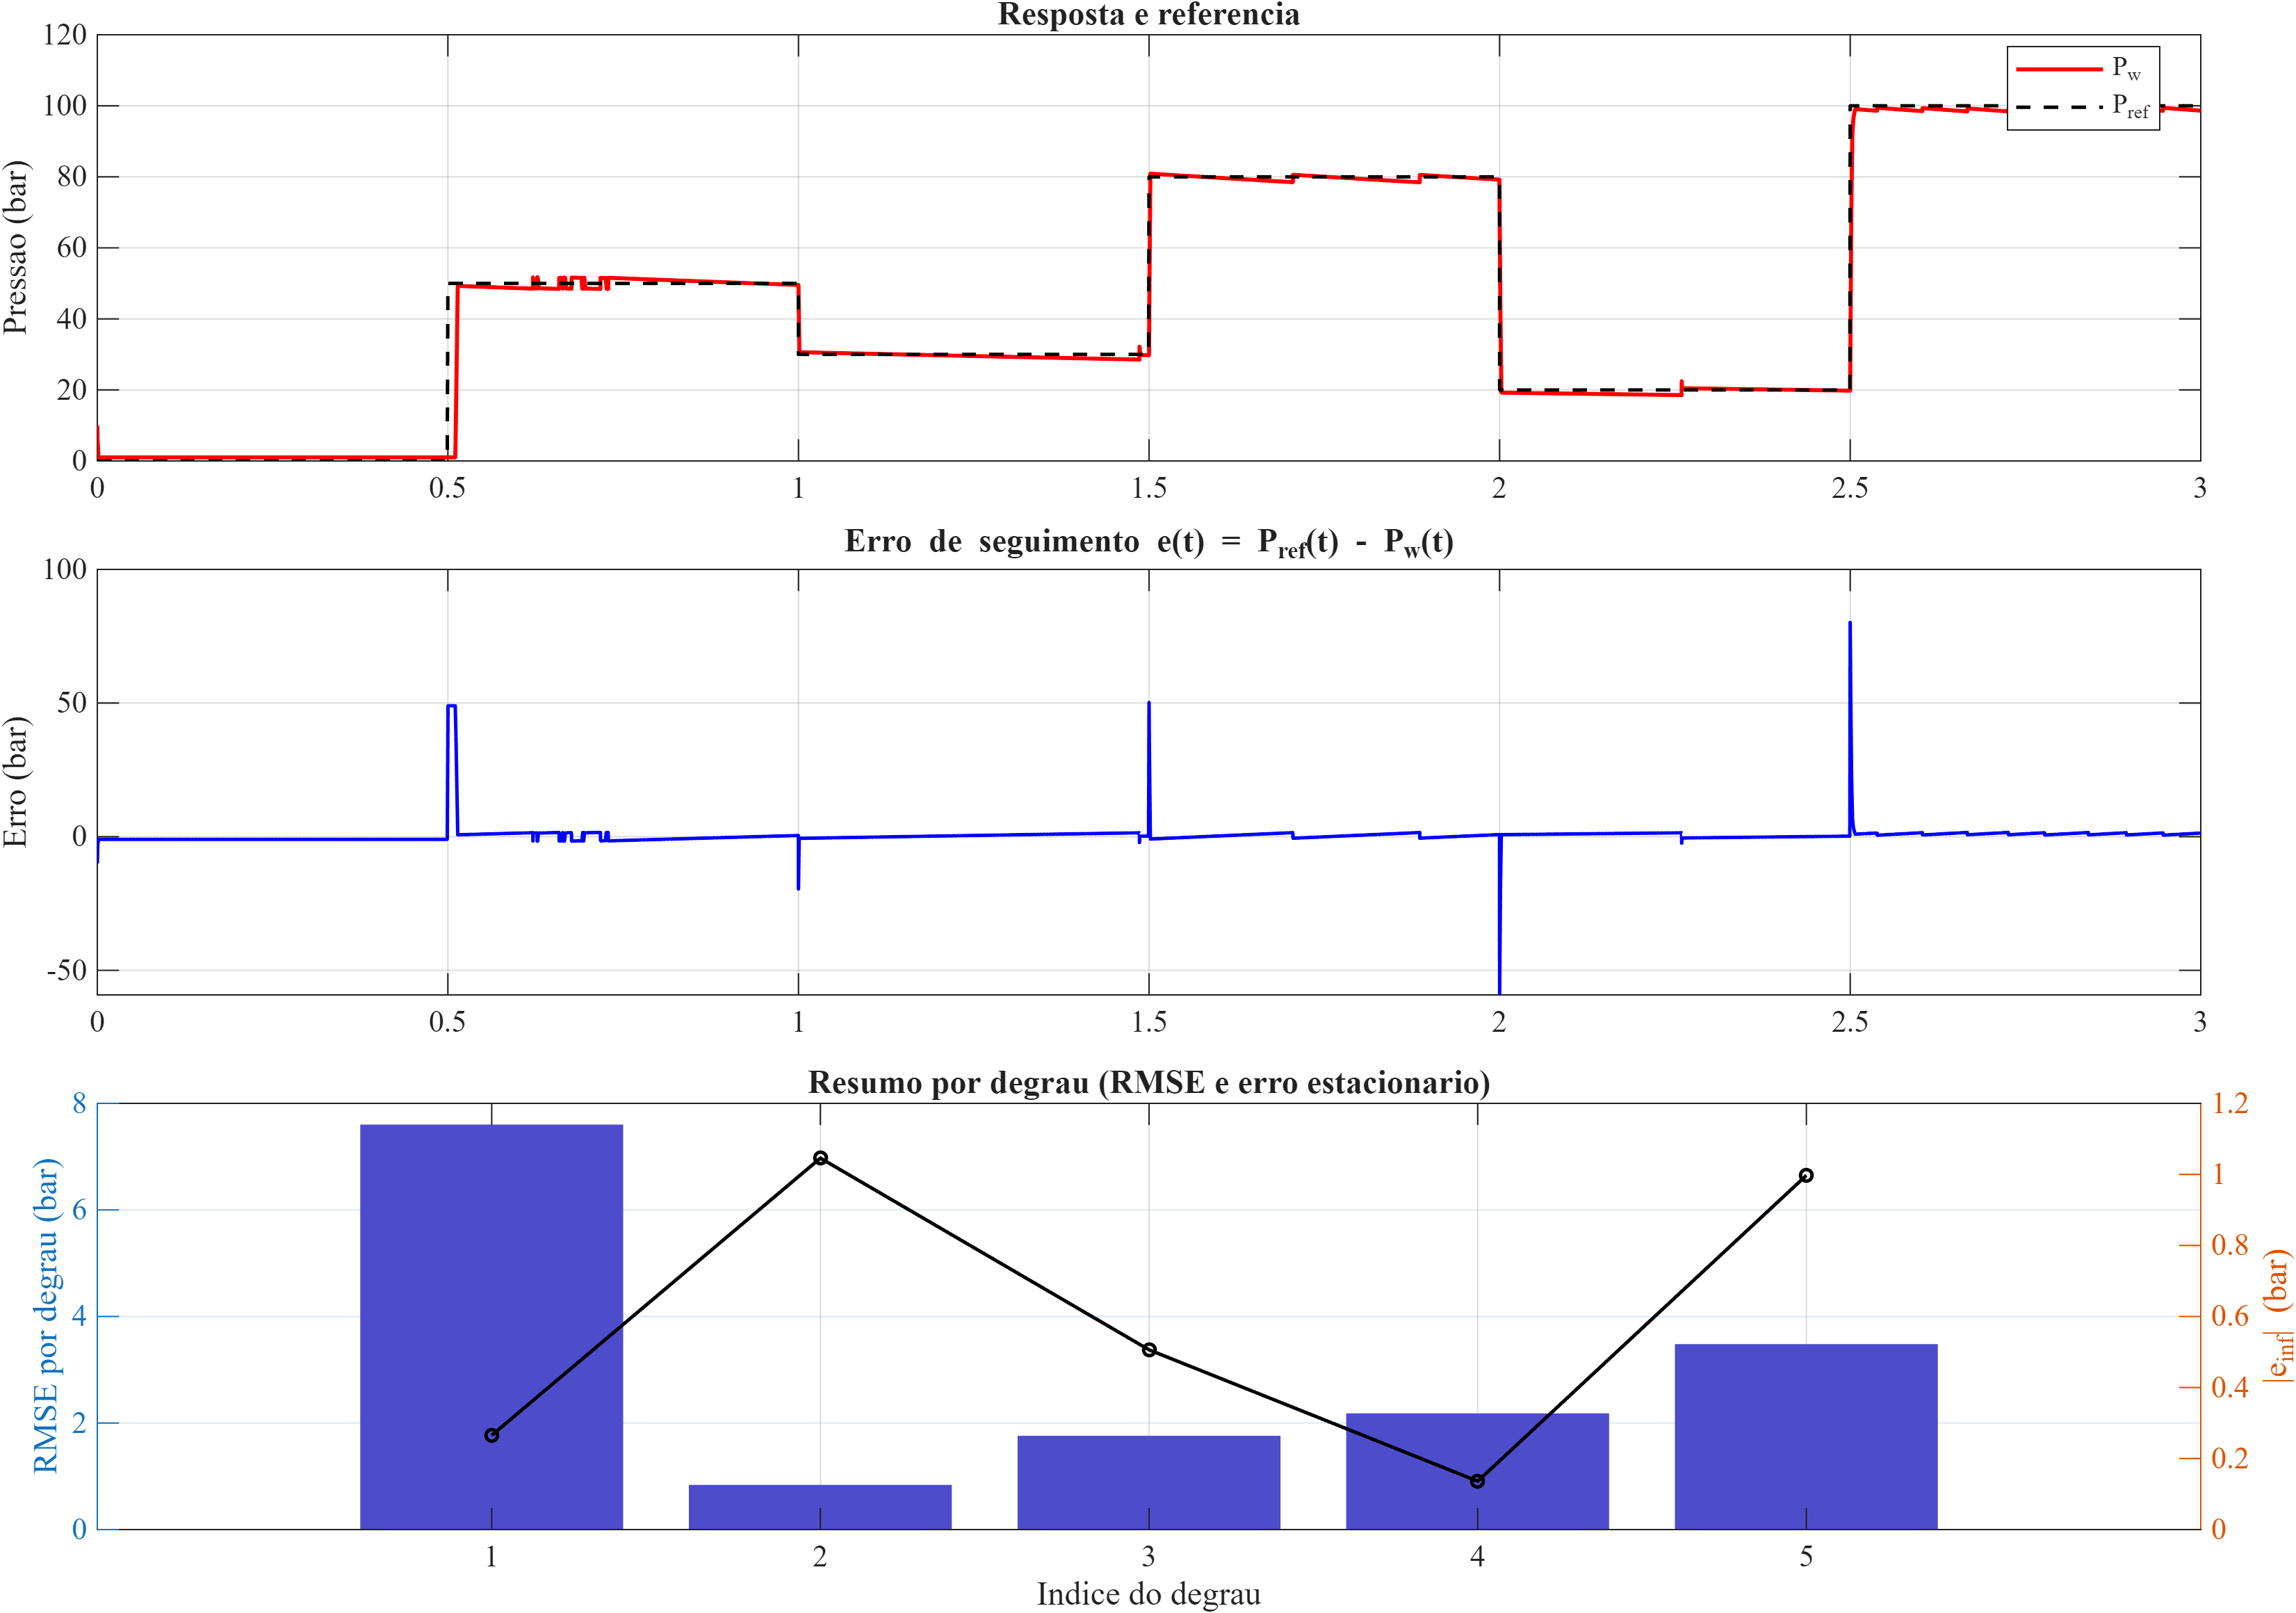
\includegraphics[width=8.4cm]{artigo_item01_metricas_tracking.png}
         \caption{Métricas de seguimento organizadas por degrau: resposta, erro e resumo por patamar.}
         \label{fig:artigo_item01_metricas_tracking}
      \end{center}
   \end{figure}

   A Figura~\ref{fig:artigo_item01_metricas_tracking} sintetiza o comportamento do seguidor de pressão ao longo do ensaio de múltiplos degraus. Observa-se que a resposta ($P_w$) acompanha a referência ($P_{ref}$) com bom alinhamento visual, apresentando apenas diferenças mais significativas nos instantes de transição entre patamares. O gráfico de erro de seguimento ($e(t)=P_{ref}(t)-P_w(t)$) evidencia picos concentrados nos degraus e valores reduzidos em regime, o que é coerente com o perfil de atuação do controlador LQI com observador.

   O resumo por degrau, em termos de erro RMS segmentado e erro estacionário, mostra que as métricas se mantêm em faixas estreitas ao longo dos cinco patamares. Em particular, os valores de erro RMS por degrau situam-se em poucos bar, enquanto o erro estacionário permanece pequeno para todos os níveis de referência. Esses resultados indicam que o desempenho do seguidor é relativamente uniforme na faixa de operação considerada, sem degradações relevantes associadas a patamares específicos de pressão.

   \begin{figure}
      \begin{center}
         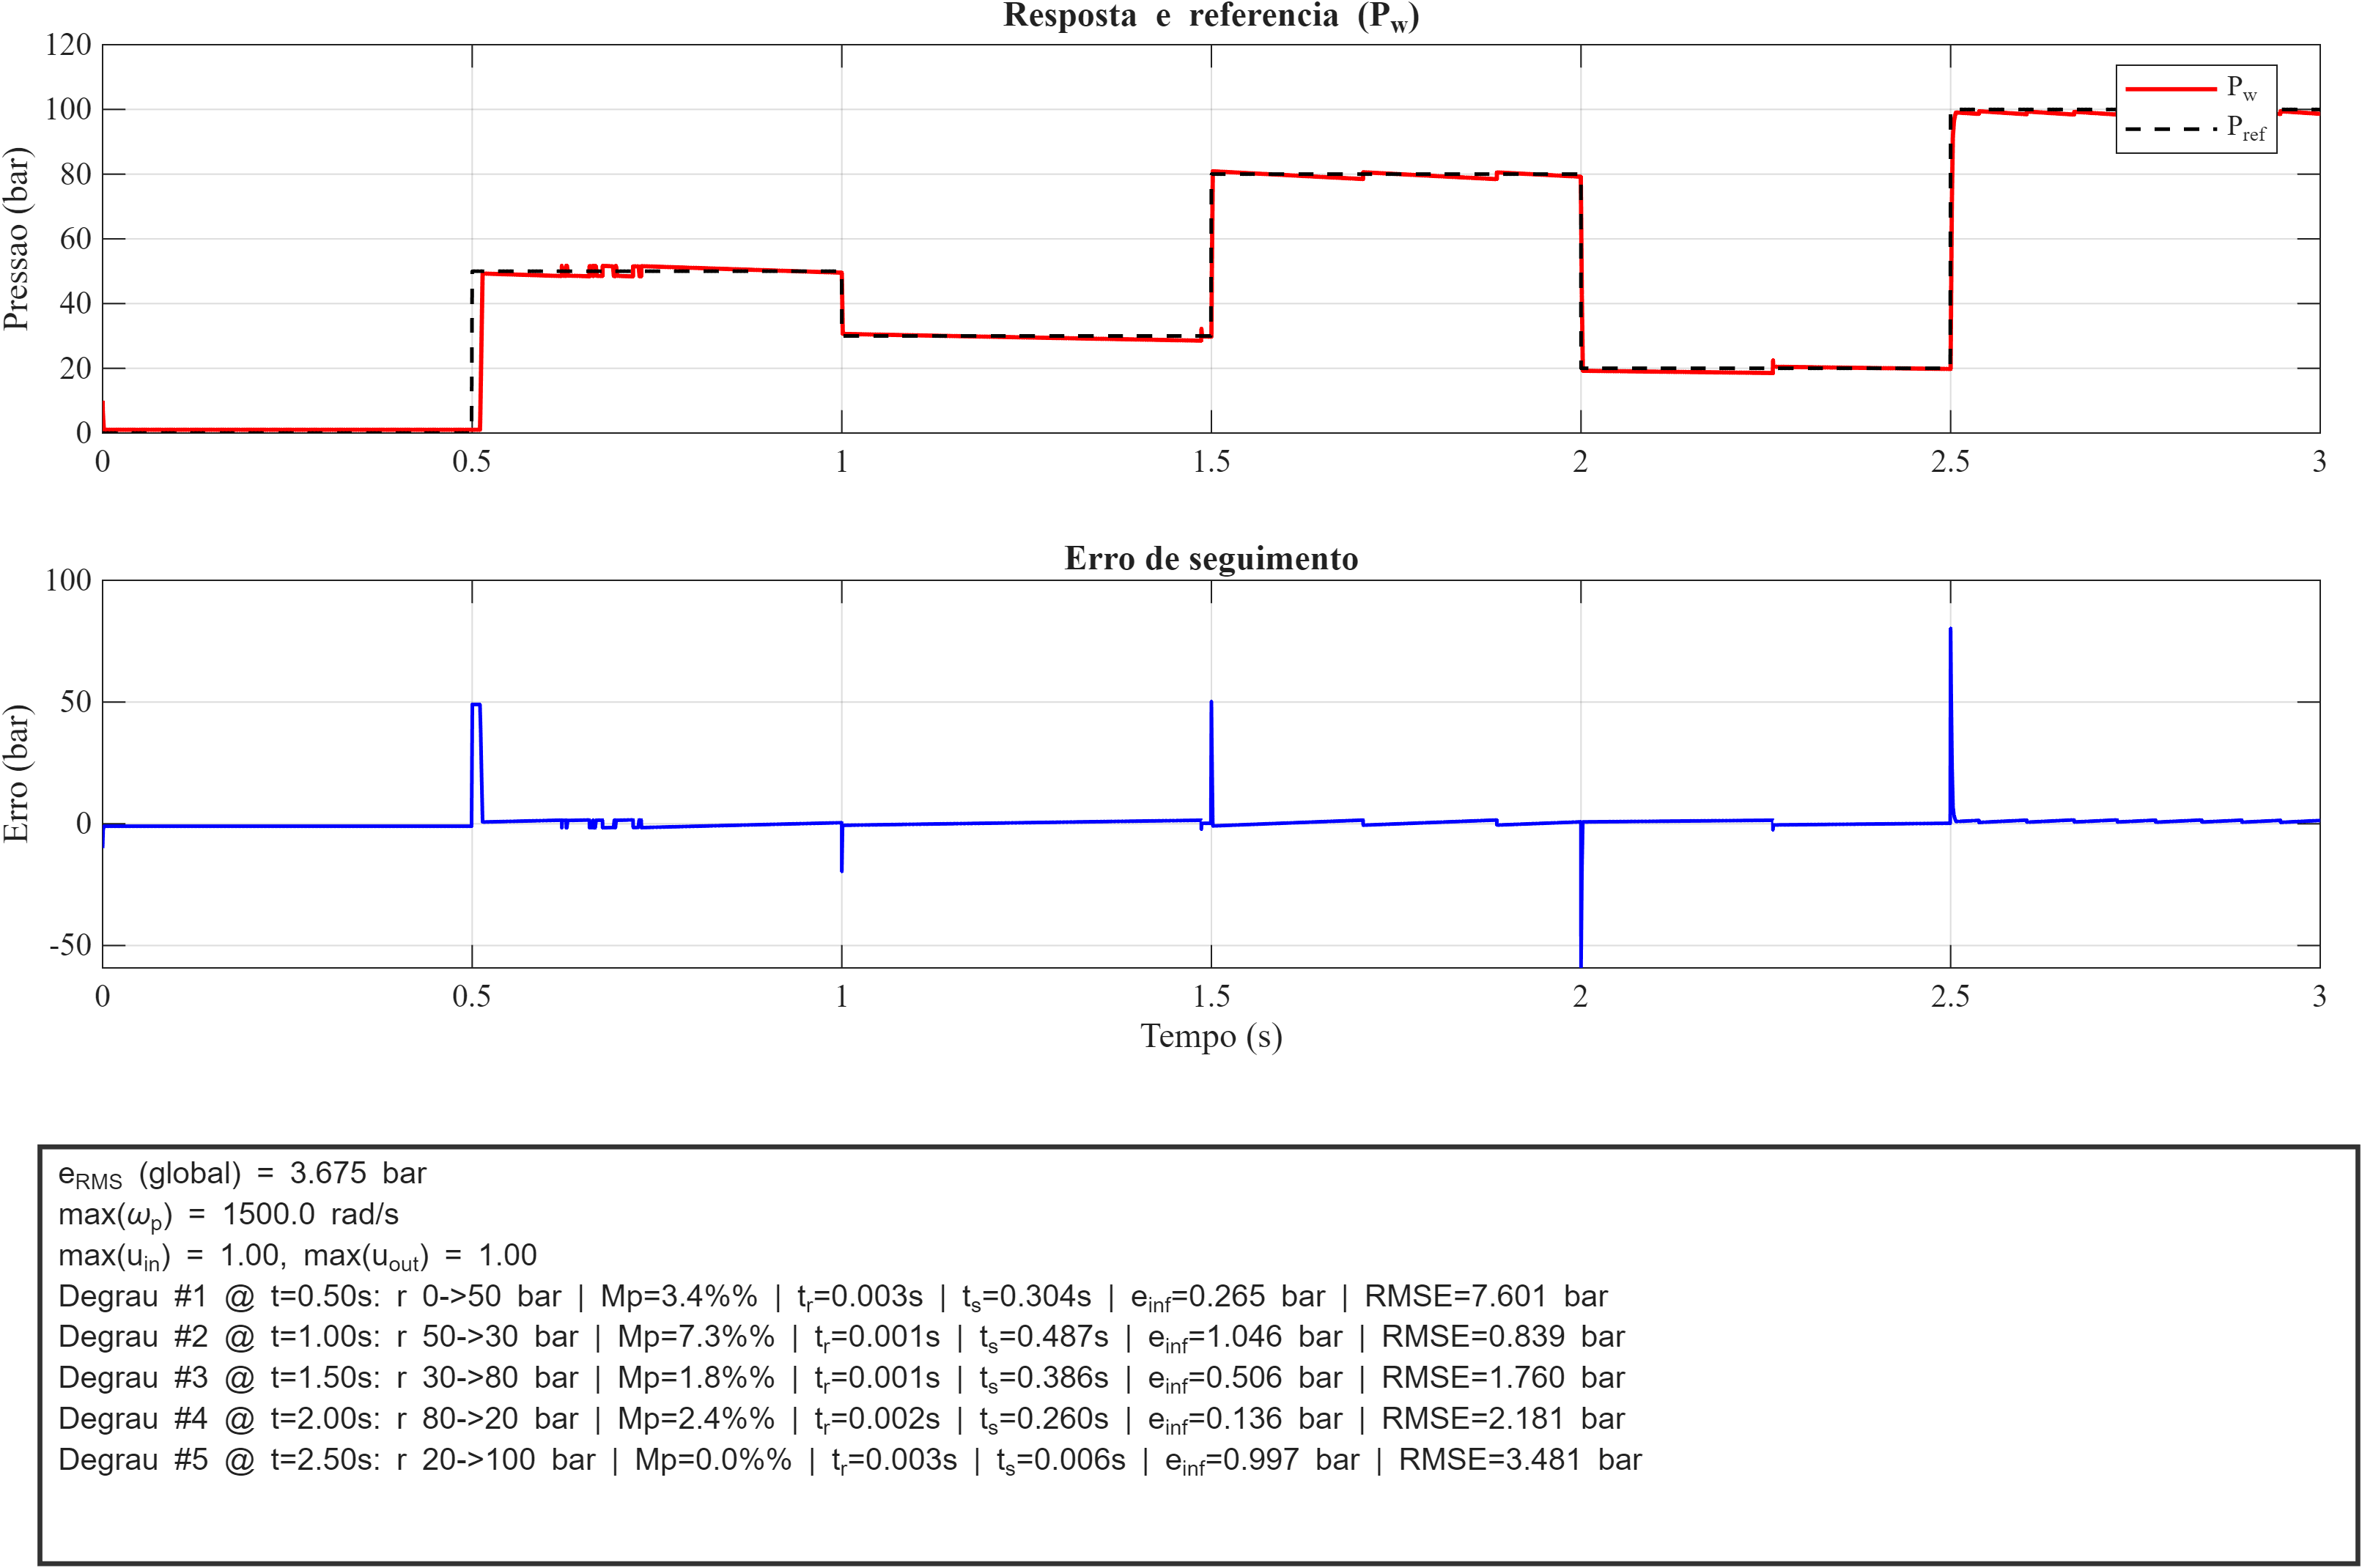
\includegraphics[width=8.4cm]{artigo_item01_metricas_desempenho.png}
         \caption{Resumo numérico de desempenho (erro global e métricas por degrau) extraído das curvas em malha fechada.}
         \label{fig:artigo_item01_metricas_desempenho}
      \end{center}
   \end{figure}

   A Figura~\ref{fig:artigo_item01_metricas_desempenho} detalha as métricas de desempenho por degrau, explicitando sobressinal, tempo de subida (10--90\%), tempo de acomodação (2\%), erro estacionário e erro RMS segmentado. Os valores numéricos obtidos reforçam a impressão qualitativa da Figura~\ref{fig:artigo_item01_metricas_tracking}: os sobressinais permanecem modestos, com valores típicos inferiores a 10\%, e os tempos de subida situam-se na ordem de algumas centenas de milissegundos. Os tempos de acomodação também se mantêm em faixas compatíveis com a dinâmica esperada de um modulador eletro-hidráulico automotivo.

   Do ponto de vista de seguimento em regime, os erros estacionários por patamar são reduzidos, tipicamente inferiores a 1~bar em magnitude. Em conjunto com o erro RMS por degrau, esses resultados sugerem que a estrutura de controle LQI com observador consegue conciliar boa rapidez de resposta com precisão em regime, para um conjunto de transições de pressão representativo de uma demanda típica de sistemas ABS/ESC.

   As Figuras~\ref{fig:artigo_item01_metricas_tracking}--\ref{fig:artigo_item01_metricas_desempenho} organizam o seguimento por degraus e tornam explícitas métricas usuais (erro RMS, sobressinal e tempos característicos), separando transientes e regime sem exigir estimativas visuais diretas.
}{ }

\IfFileExists{artigo_item02_dpdt_saturacao.png}{%
   \begin{figure}
      \begin{center}
         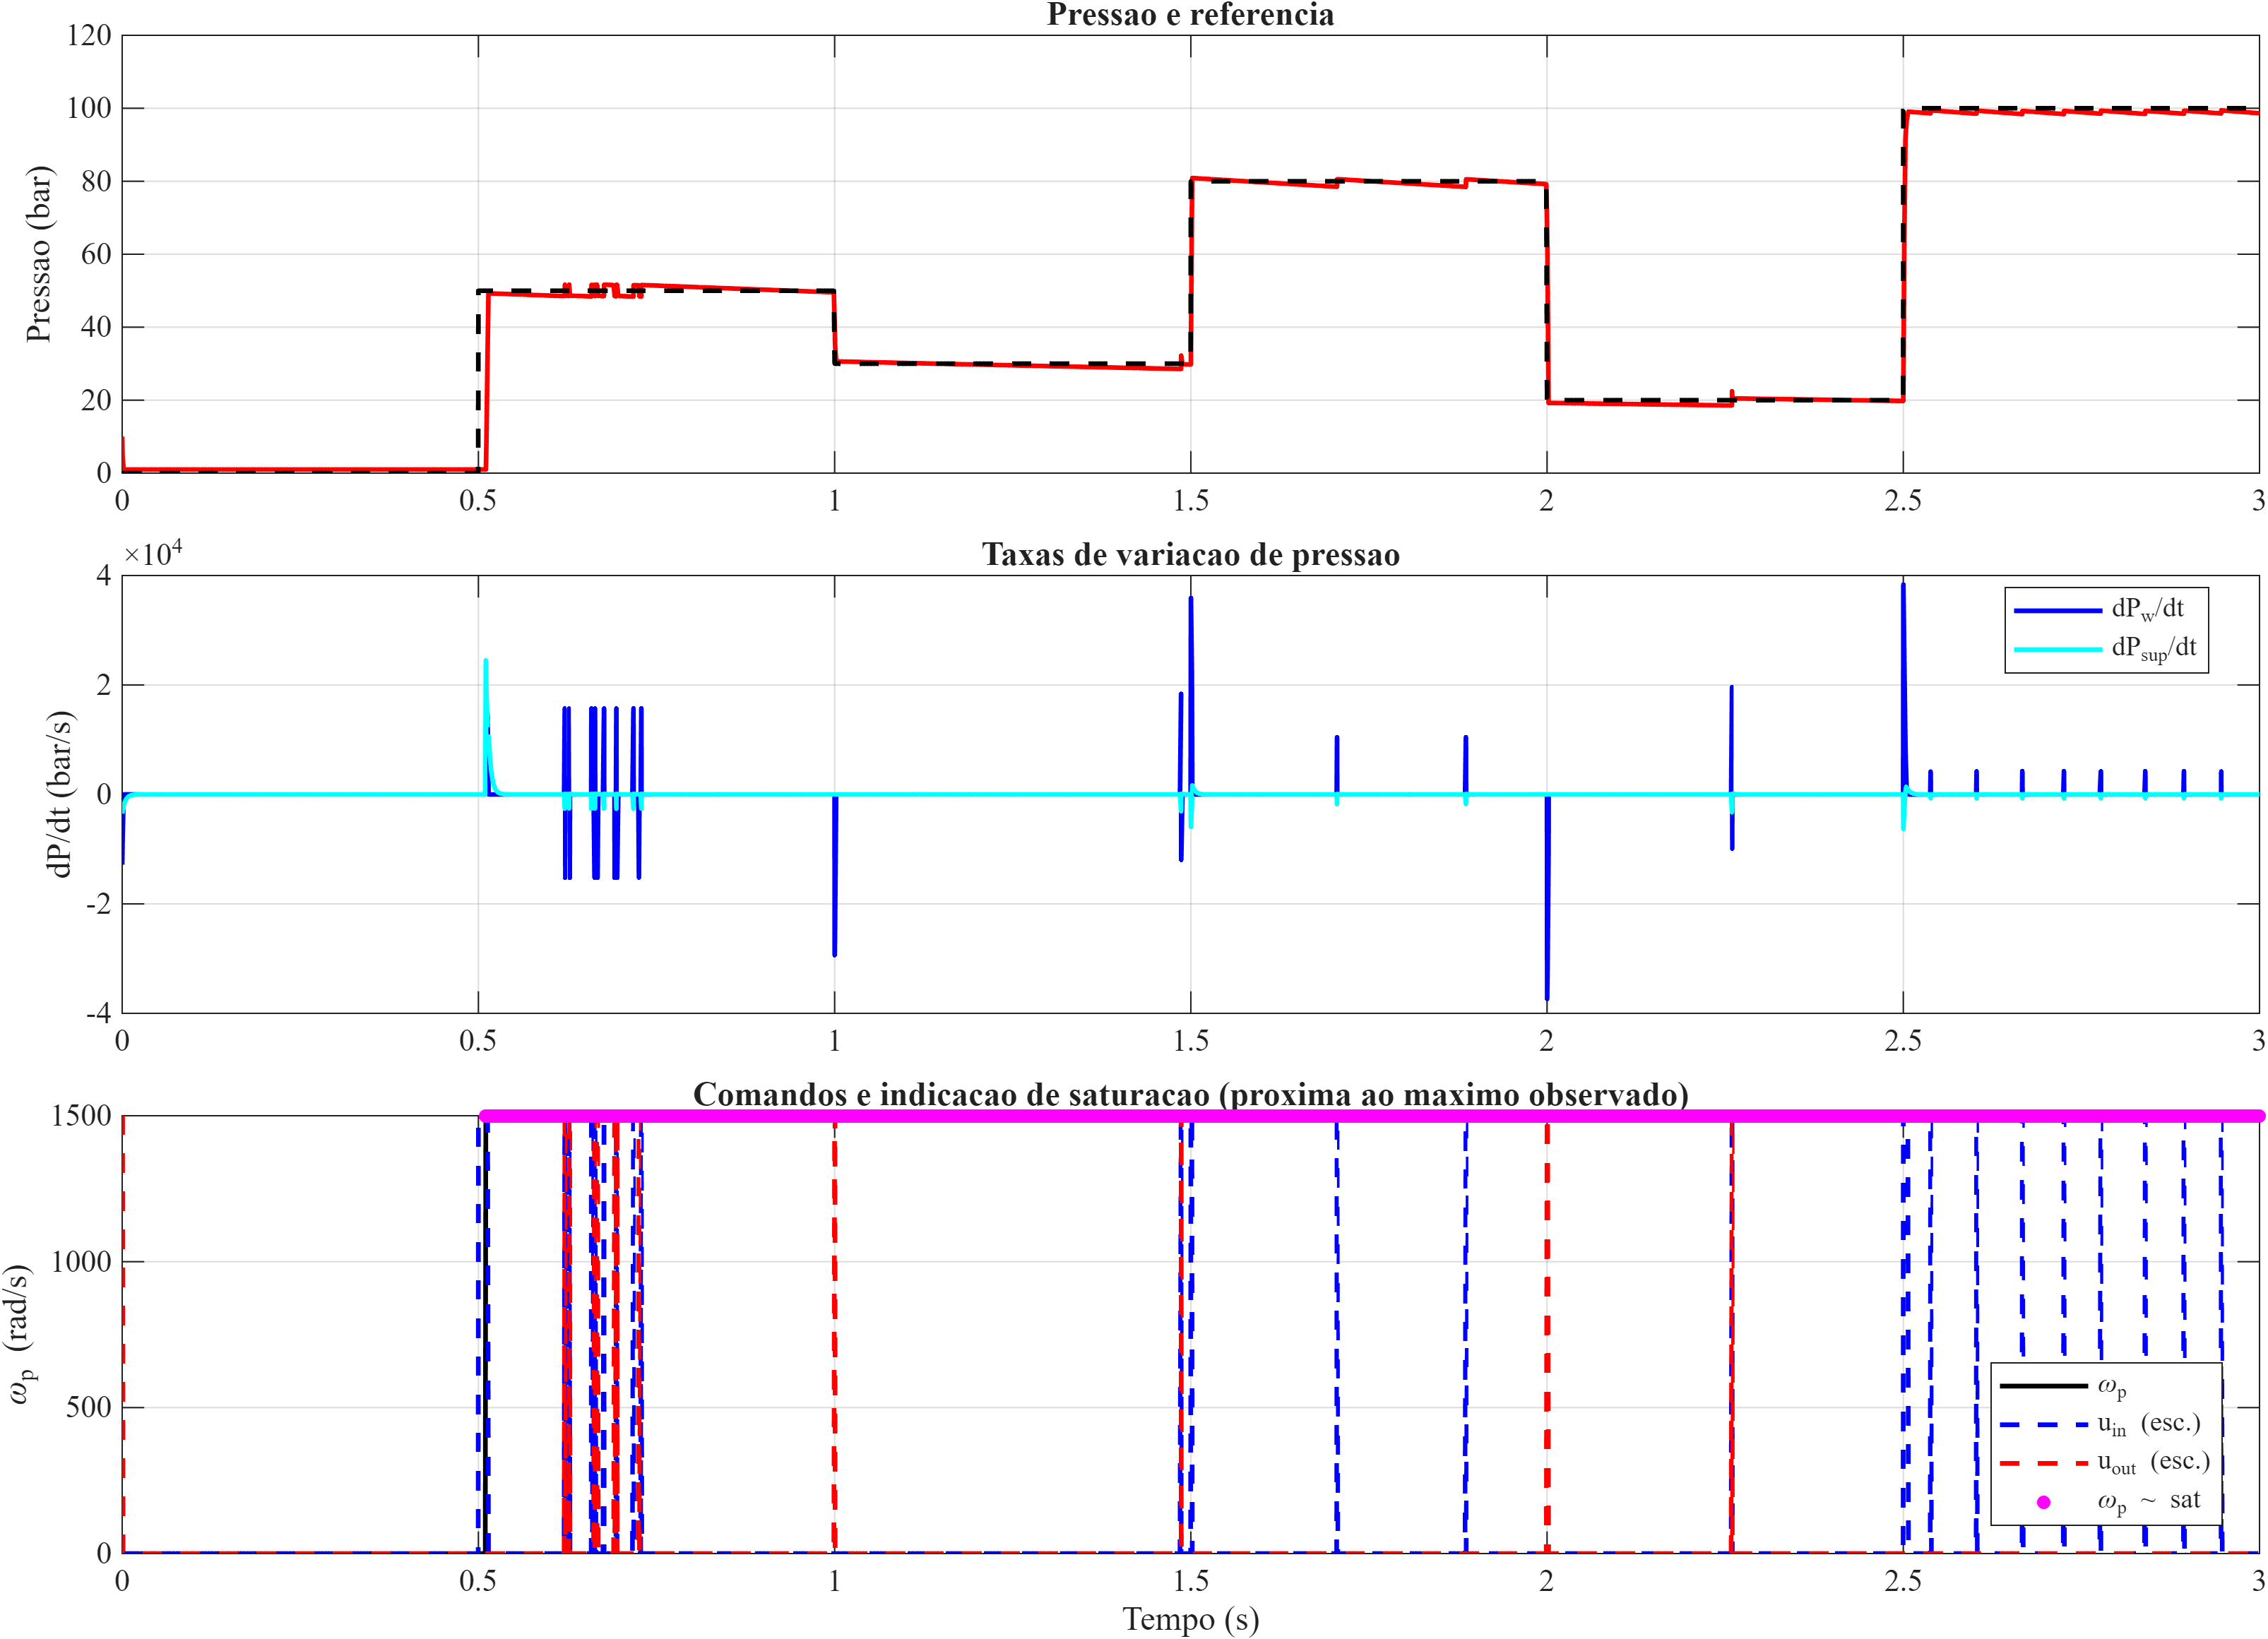
\includegraphics[width=8.4cm]{artigo_item02_dpdt_saturacao.png}
         \caption{Taxas de variação de pressão e indicação de saturação do comando (próximo ao máximo observado).}
         \label{fig:artigo_item02_dpdt_saturacao}
      \end{center}
   \end{figure}

   A análise de $\mathrm{d}P/\mathrm{d}t$ (Figura~\ref{fig:artigo_item02_dpdt_saturacao}) complementa as métricas temporais ao explicitar limites dinâmicos do atuador hidráulico. Como as vazões seguem leis dependentes de $\sqrt{\Delta P}$ e o ganho efetivo da dinâmica depende de $\beta/V$, a presença de saturações e de limitações de diferencial de pressão tende a impor um teto para $|\mathrm{d}P/\mathrm{d}t|$, que deve ser discutido separadamente do erro de seguimento.

   A Figura~\ref{fig:artigo_item02_dpdt_saturacao} permite explicitar de forma mais clara os limites físicos do sistema. Observa-se que, mesmo quando o comando da bomba se aproxima do limite superior de operação, os picos de $\left|\mathrm{d}P_w/\mathrm{d}t\right|$ permanecem confinados a uma faixa relativamente estreita, repetindo-se com amplitudes semelhantes em diferentes degraus de referência.

   Esse comportamento indica que a taxa máxima de variação de pressão é imposta primariamente pela dinâmica hidráulica (compressibilidade, volumes efetivos e áreas de passagem), e não apenas pelo esforço de controle. Em outras palavras, há um teto físico para $\left|\mathrm{d}P/\mathrm{d}t\right|$ que o controlador não consegue superar, ainda que sature o comando da bomba. Essa constatação é relevante para o dimensionamento de moduladores hidráulicos, pois sugere que, a partir de certo ponto, aumentos adicionais de esforço de atuação não se traduzem em respostas de pressão mais rápidas.
}{ }

\IfFileExists{artigo_item03_assimetria_subida_descida.png}{%
   \begin{figure}
      \begin{center}
         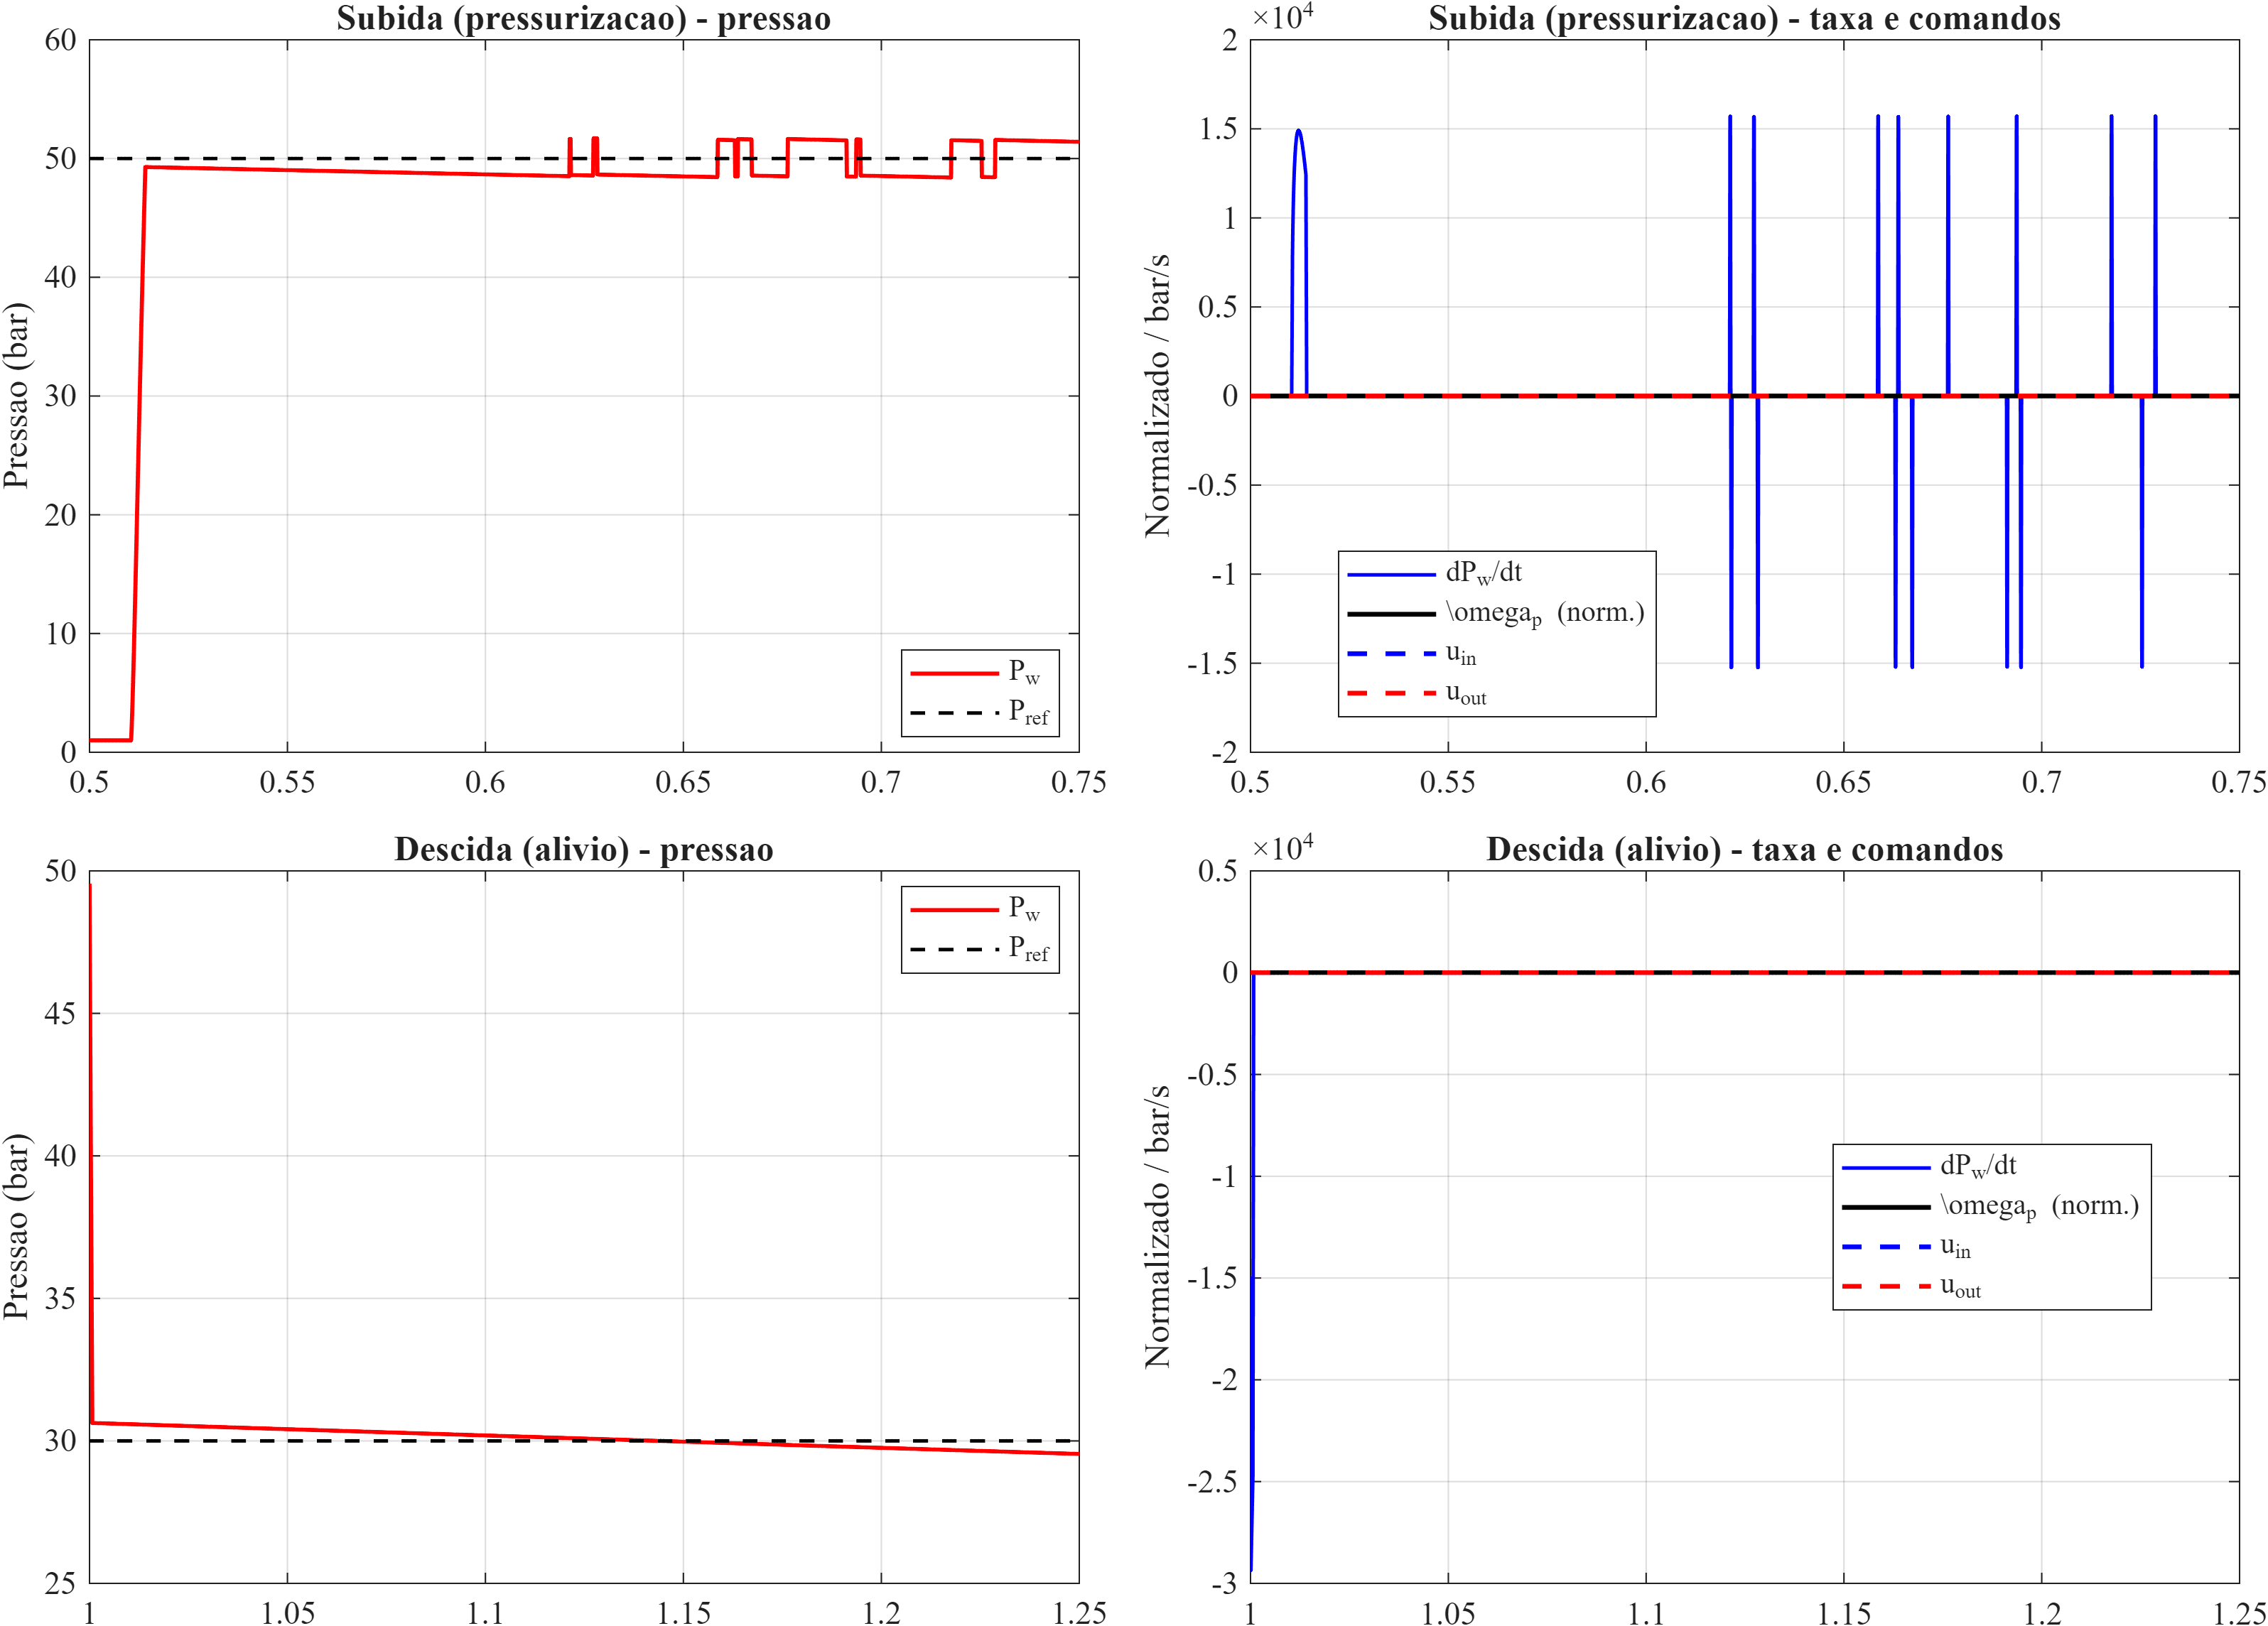
\includegraphics[width=8.4cm]{artigo_item03_assimetria_subida_descida.png}
         \caption{Comparação entre transientes de pressurização e alívio: resposta, taxa $\mathrm{d}P_w/\mathrm{d}t$ e comandos.}
         \label{fig:artigo_item03_assimetria_subida_descida}
      \end{center}
   \end{figure}

   A Figura~\ref{fig:artigo_item03_assimetria_subida_descida} evidencia assimetria entre pressurização e alívio, comportamento esperado quando os caminhos de fluxo e as condições de $\Delta P$ diferem nos dois sentidos. Essa leitura é importante porque o desempenho pode ser limitado pela física do circuito (e não pelo regulador), e deve ser reportado de forma objetiva antes de extrapolar conclusões sobre o controlador \cite{Lv2014,ChenLv2017}.
}{ }

\IfFileExists{artigo_item04_ripple_fft.png}{%
   \begin{figure}
      \begin{center}
         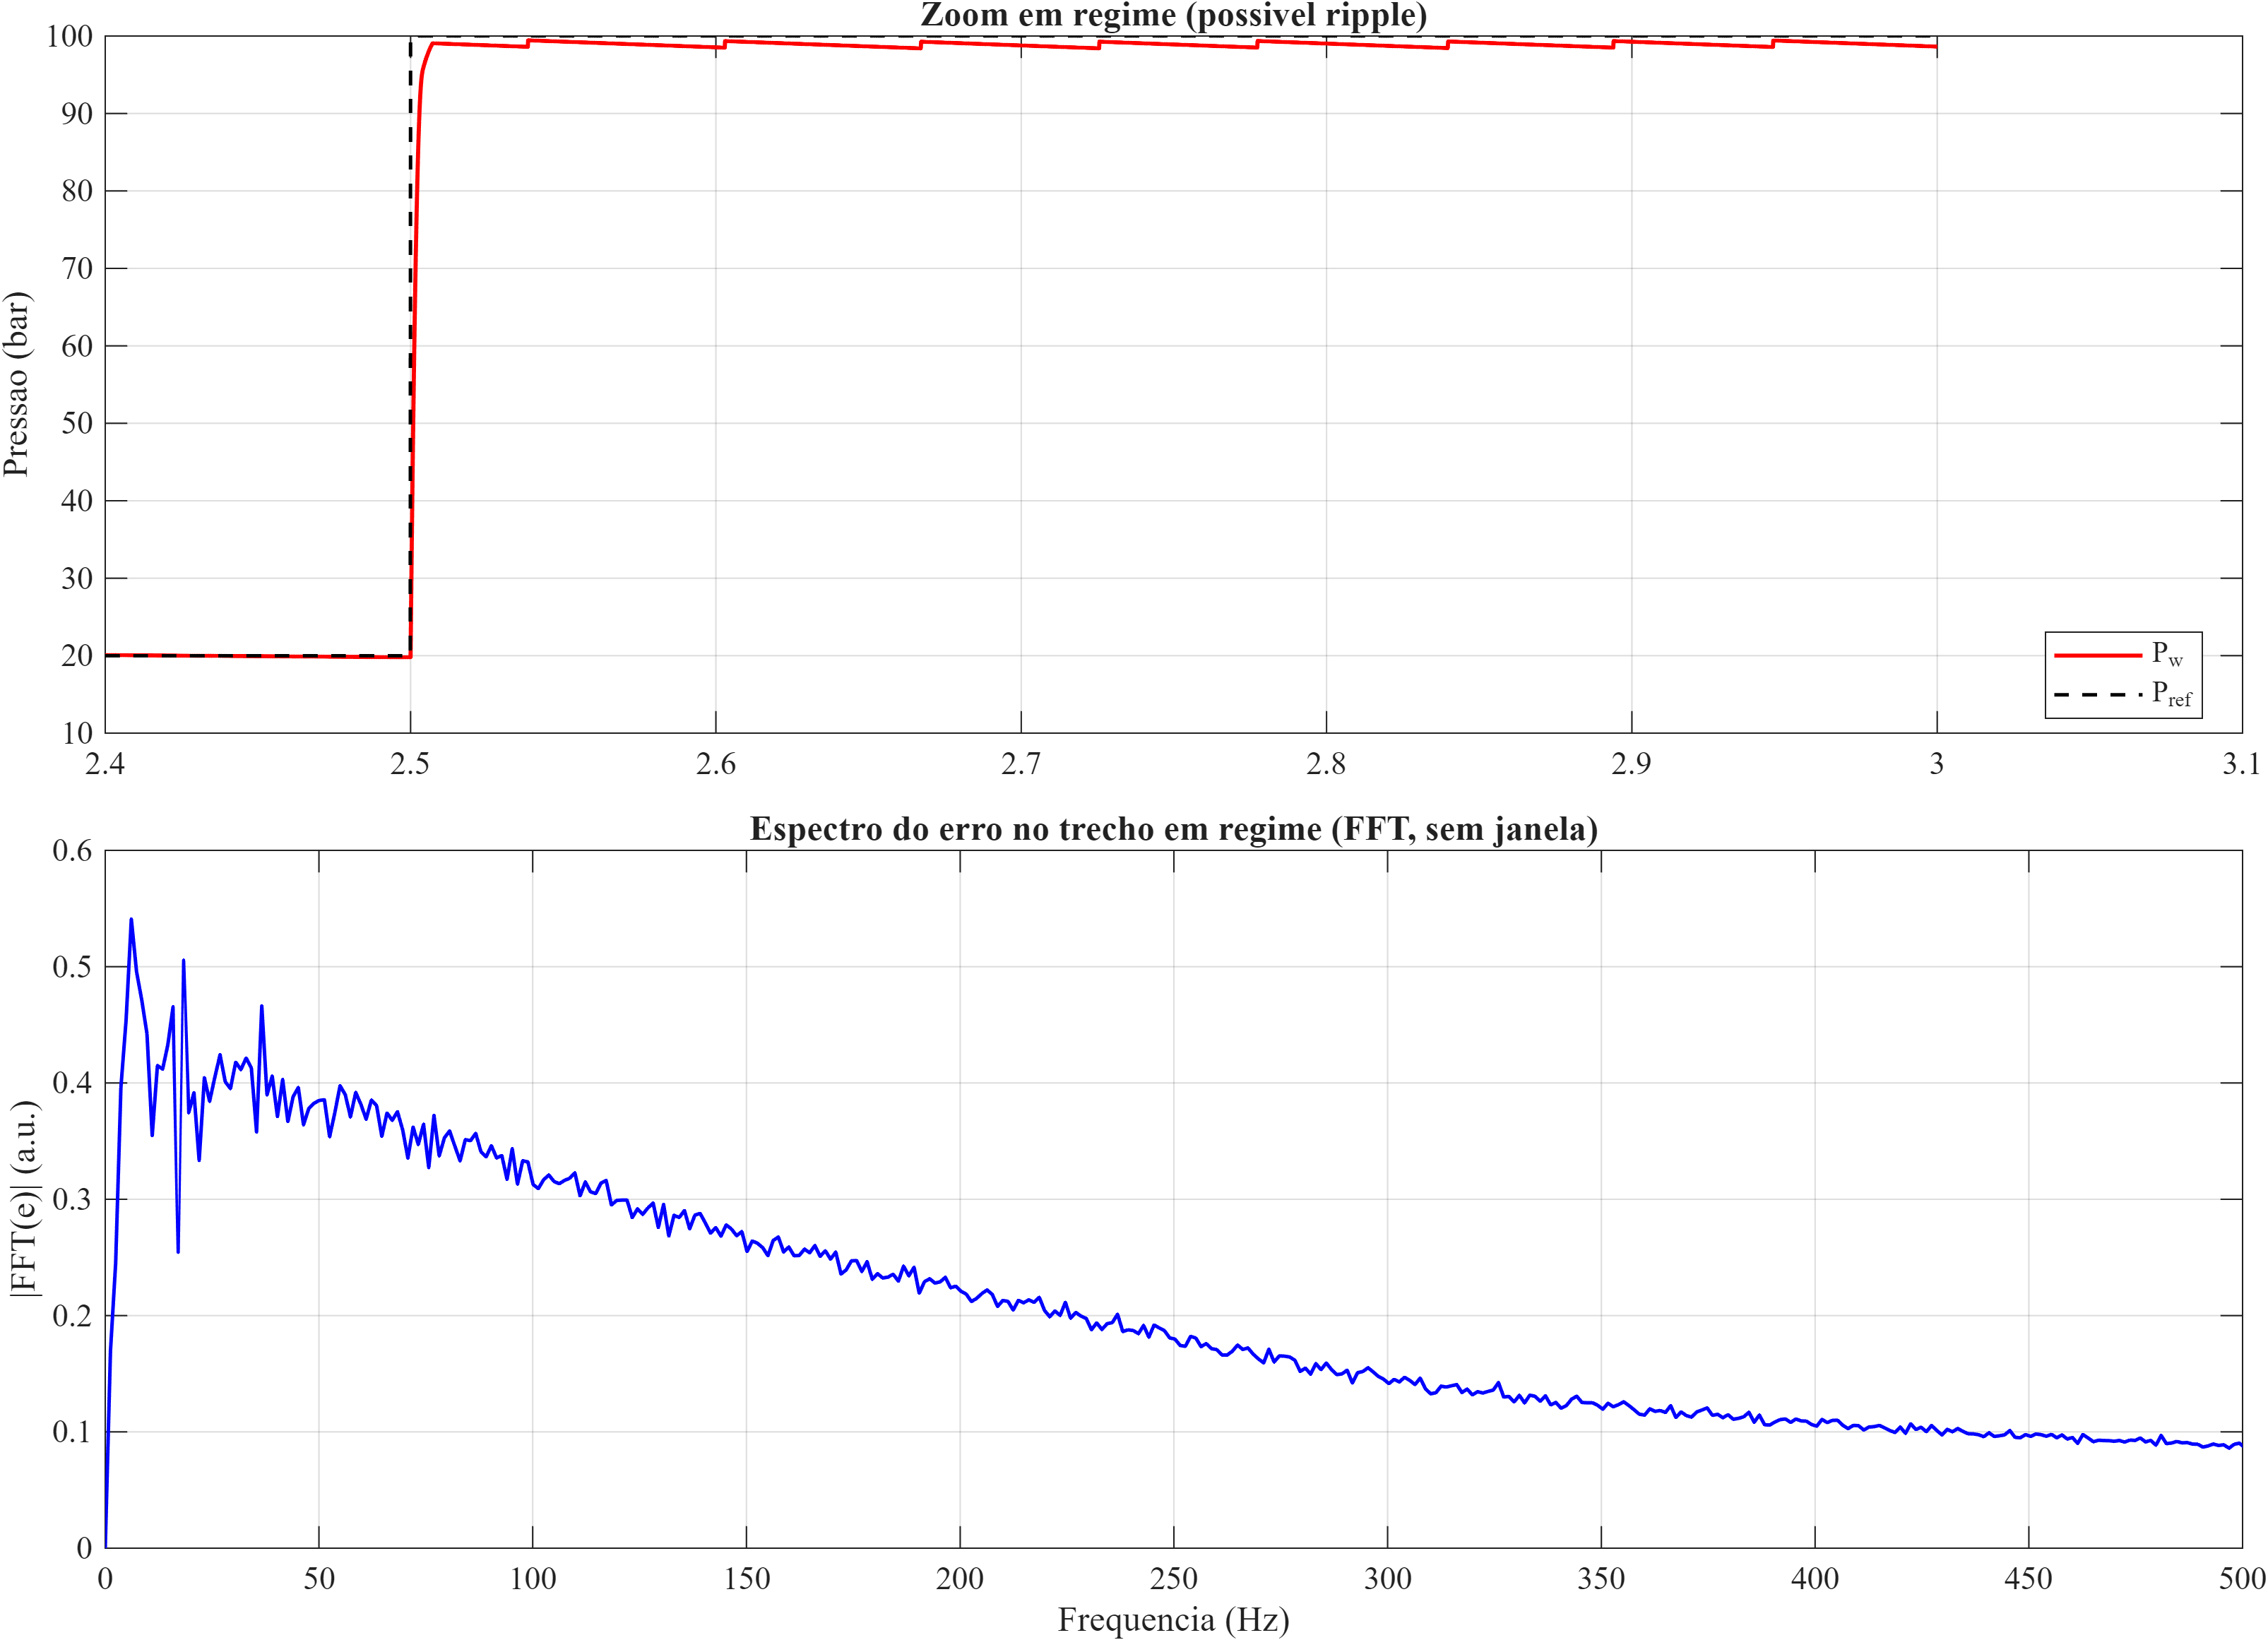
\includegraphics[width=8.4cm]{artigo_item04_ripple_fft.png}
         \caption{Avaliação de ondulação em regime (ripple) e conteúdo espectral do erro em um trecho de patamar.}
         \label{fig:artigo_item04_ripple_fft}
      \end{center}
   \end{figure}

   Para além do erro médio, a ondulação em regime (Figura~\ref{fig:artigo_item04_ripple_fft}) caracteriza flutuações associadas à lógica discreta de válvulas e ao período de amostragem. A inspeção temporal e espectral do erro em patamar ajuda a distinguir erro de seguimento lento de oscilações de alta frequência que podem elevar comutação e esforço de atuação.
}{ }

\IfFileExists{artigo_item05_validacao_linearizacao.png}{%
   \begin{figure}
      \begin{center}
         \includegraphics[width=8.4cm]{artigo_item05_validacao_linearizacao.png}
         \caption{Checagem local de consistência: planta não linear versus modelo linearizado em janela de operação.}
         \label{fig:artigo_item05_validacao_linearizacao}
      \end{center}
   \end{figure}

   Como a síntese do LQI depende da linearização local, a Figura~\ref{fig:artigo_item05_validacao_linearizacao} é usada como checagem de consistência em pequena vizinhança do ponto de operação. Diferenças residuais entre as curvas indicam o grau de não linearidade efetivamente excitado e ajudam a delimitar a faixa de validade do projeto linear, sem sugerir equivalência global entre modelos.
}{ }

\IfFileExists{artigo_item06_sensibilidade_parametrica.png}{%
   \begin{figure}
      \begin{center}
         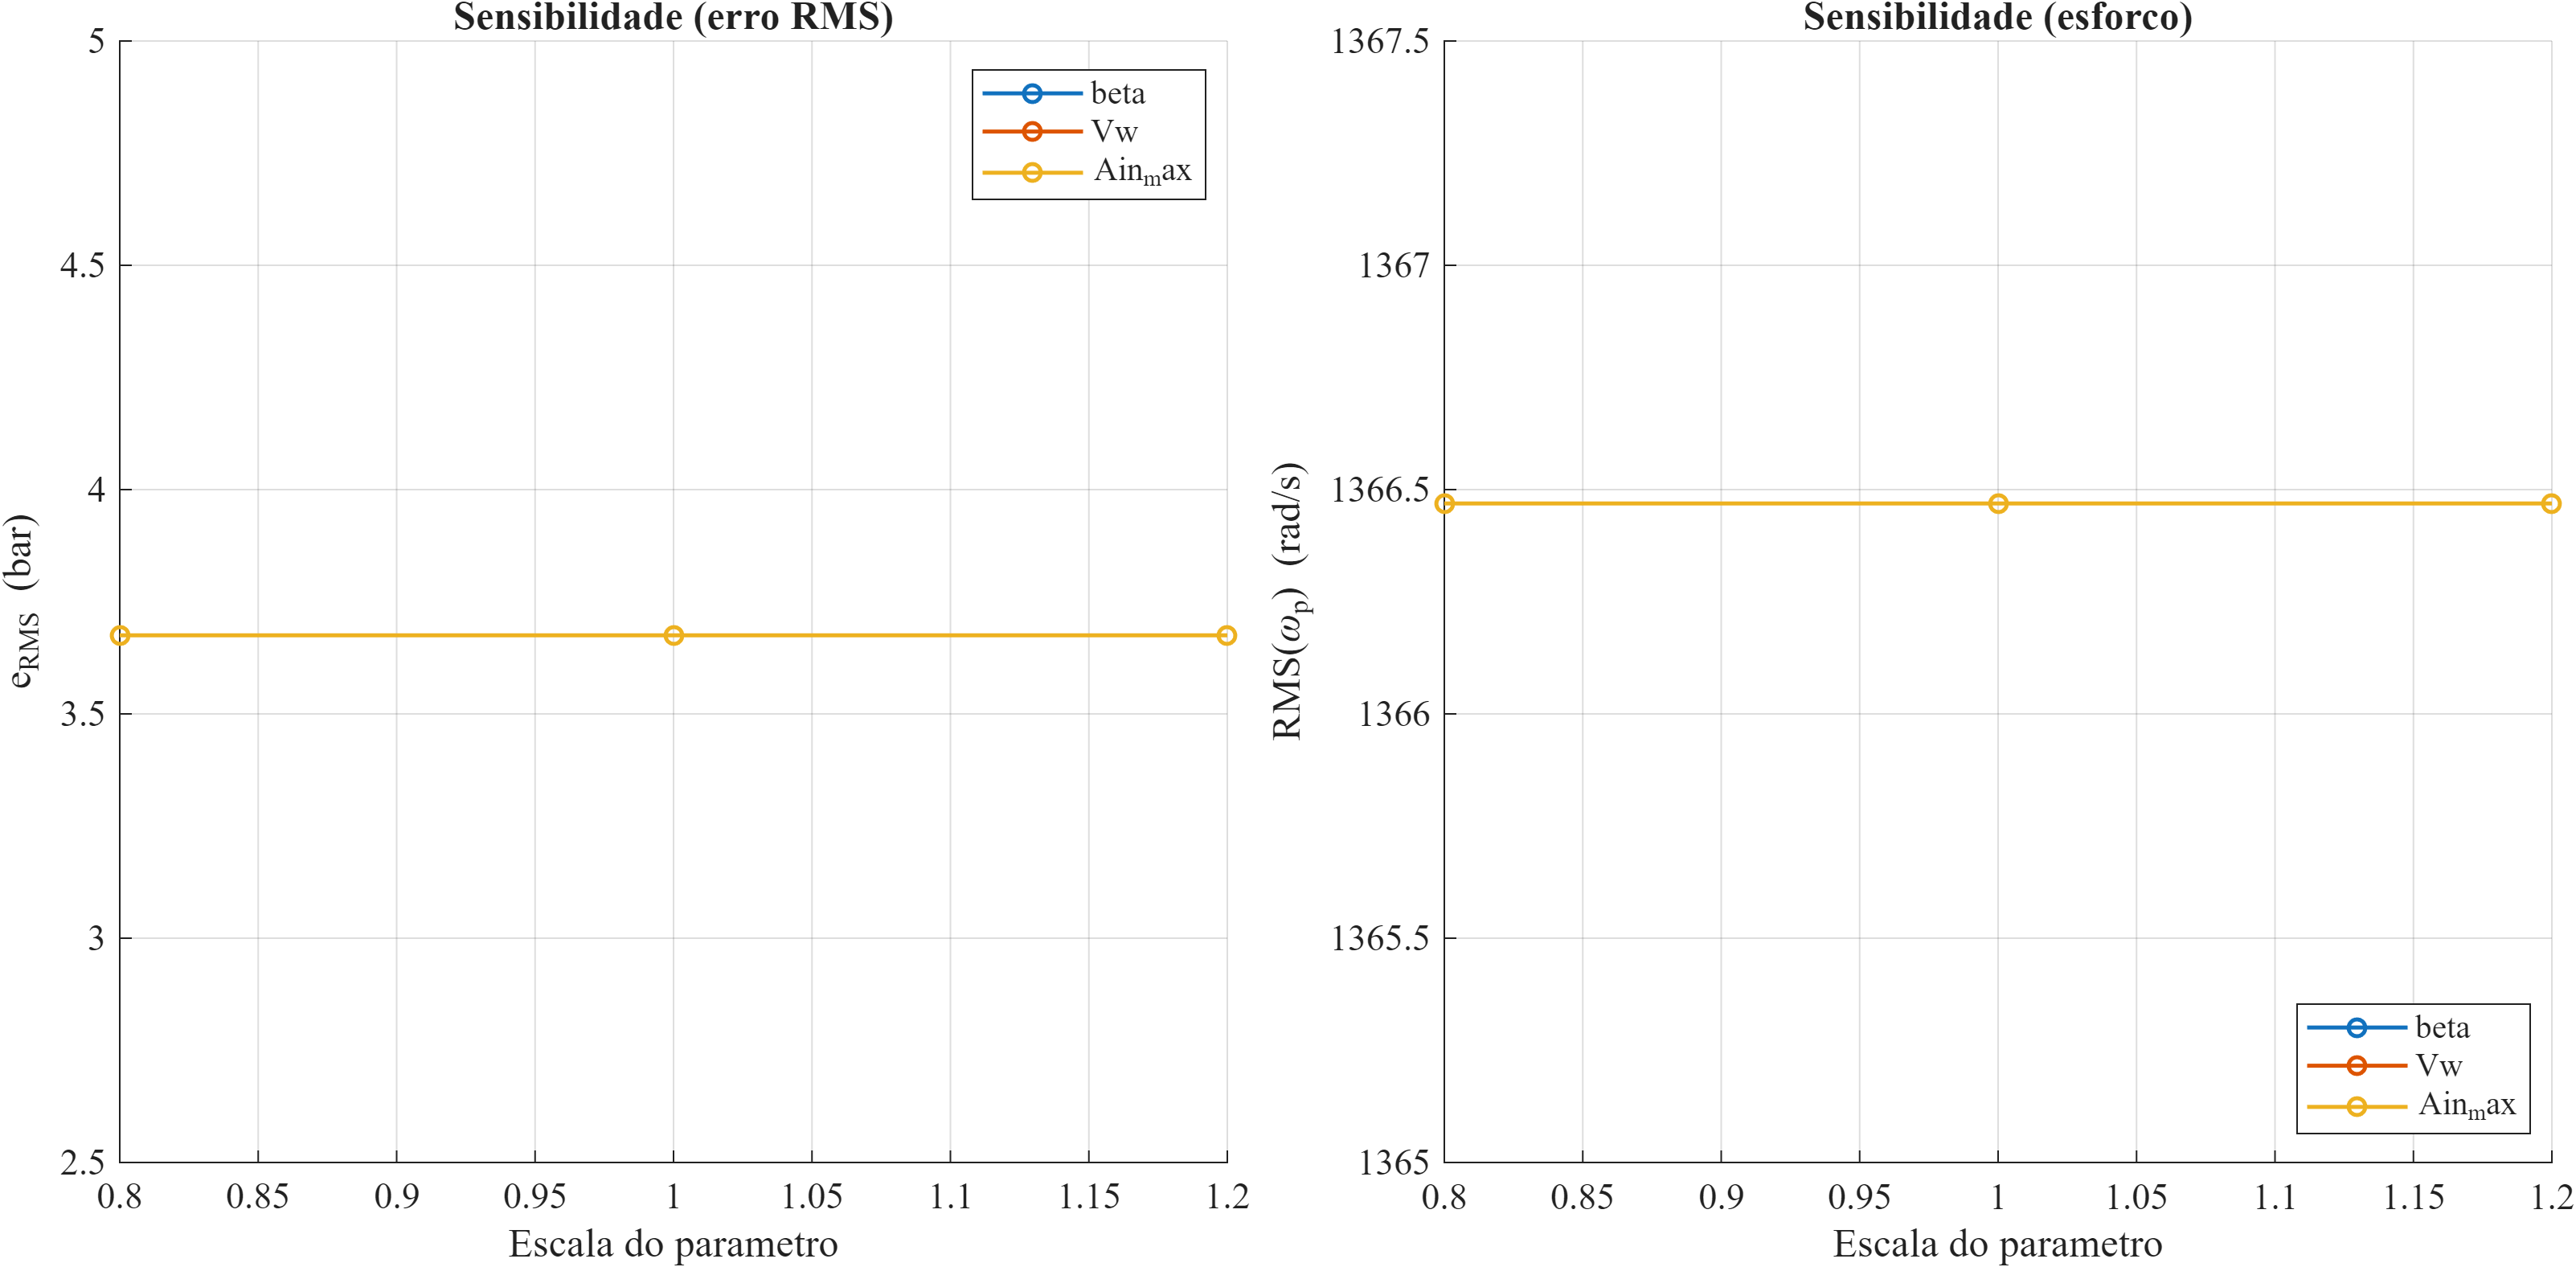
\includegraphics[width=8.4cm]{artigo_item06_sensibilidade_parametrica.png}
         \caption{Sensibilidade paramétrica (exemplo): impacto de variações em parâmetros hidráulicos nas métricas de erro e esforço.}
         \label{fig:artigo_item06_sensibilidade_parametrica}
      \end{center}
   \end{figure}

   A robustez do conjunto modelo+controle é discutida com base em variações paramétricas em torno do caso nominal (Figura~\ref{fig:artigo_item06_sensibilidade_parametrica}), focalizando parâmetros com interpretação física direta (por exemplo, $\beta$, volumes equivalentes e áreas efetivas). Essa análise ajuda a identificar quais incertezas tendem a dominar a degradação do seguimento e quais afetam principalmente o esforço do atuador.

   A análise de sensibilidade local, apresentada na Figura~\ref{fig:artigo_item06_sensibilidade_parametrica}, mostra o efeito de variações de $\pm 20\%$ nos parâmetros $\beta$, $V_w$ e $A_{in,\max}$ sobre o erro RMS de seguimento e o esforço RMS do atuador. Observa-se que, dentro dessa faixa de variação, tanto o erro RMS quanto o RMS da velocidade da bomba permanecem quase constantes, com diferenças pouco expressivas entre os valores extremos de escala.

   Esse resultado indica que, para o cenário de ensaio considerado, o desempenho em malha fechada é pouco sensível a perturbações moderadas nesses parâmetros hidráulicos. Em outras palavras, a estrutura de controle LQI com observador confere um grau de robustez que limita o impacto de incertezas de ordem prática em $\beta$, $V_w$ e $A_{in,\max}$, ao menos na vizinhança dos valores nominais utilizados no projeto.

   A Figura~\ref{fig:artigo_item06_sensibilidade_parametrica} também sintetiza, em termos globais, o erro RMS e o esforço RMS para diferentes escalas dos parâmetros hidráulicos. Os resultados confirmam a tendência observada na análise local: as barras associadas a $\beta$, $V_w$ e $A_{in,\max}$ apresentam variação reduzida de desempenho ao longo das escalas $0{,}8$--$1{,}2$, tanto no indicador de erro quanto no indicador de esforço.

   Do ponto de vista prático, essa baixa variabilidade sugere que o sistema é capaz de manter um padrão de desempenho semelhante mesmo na presença de incertezas paramétricas típicas de projeto e fabricação. Assim, as simulações apontam para uma robustez razoável da malha de controle em relação a variações moderadas na compressibilidade efetiva, nos volumes equivalentes e na área de passagem máxima da válvula de entrada.
}{ }

\IfFileExists{artigo_item07_atrasos_tempos.png}{%
   \begin{figure}
      \begin{center}
         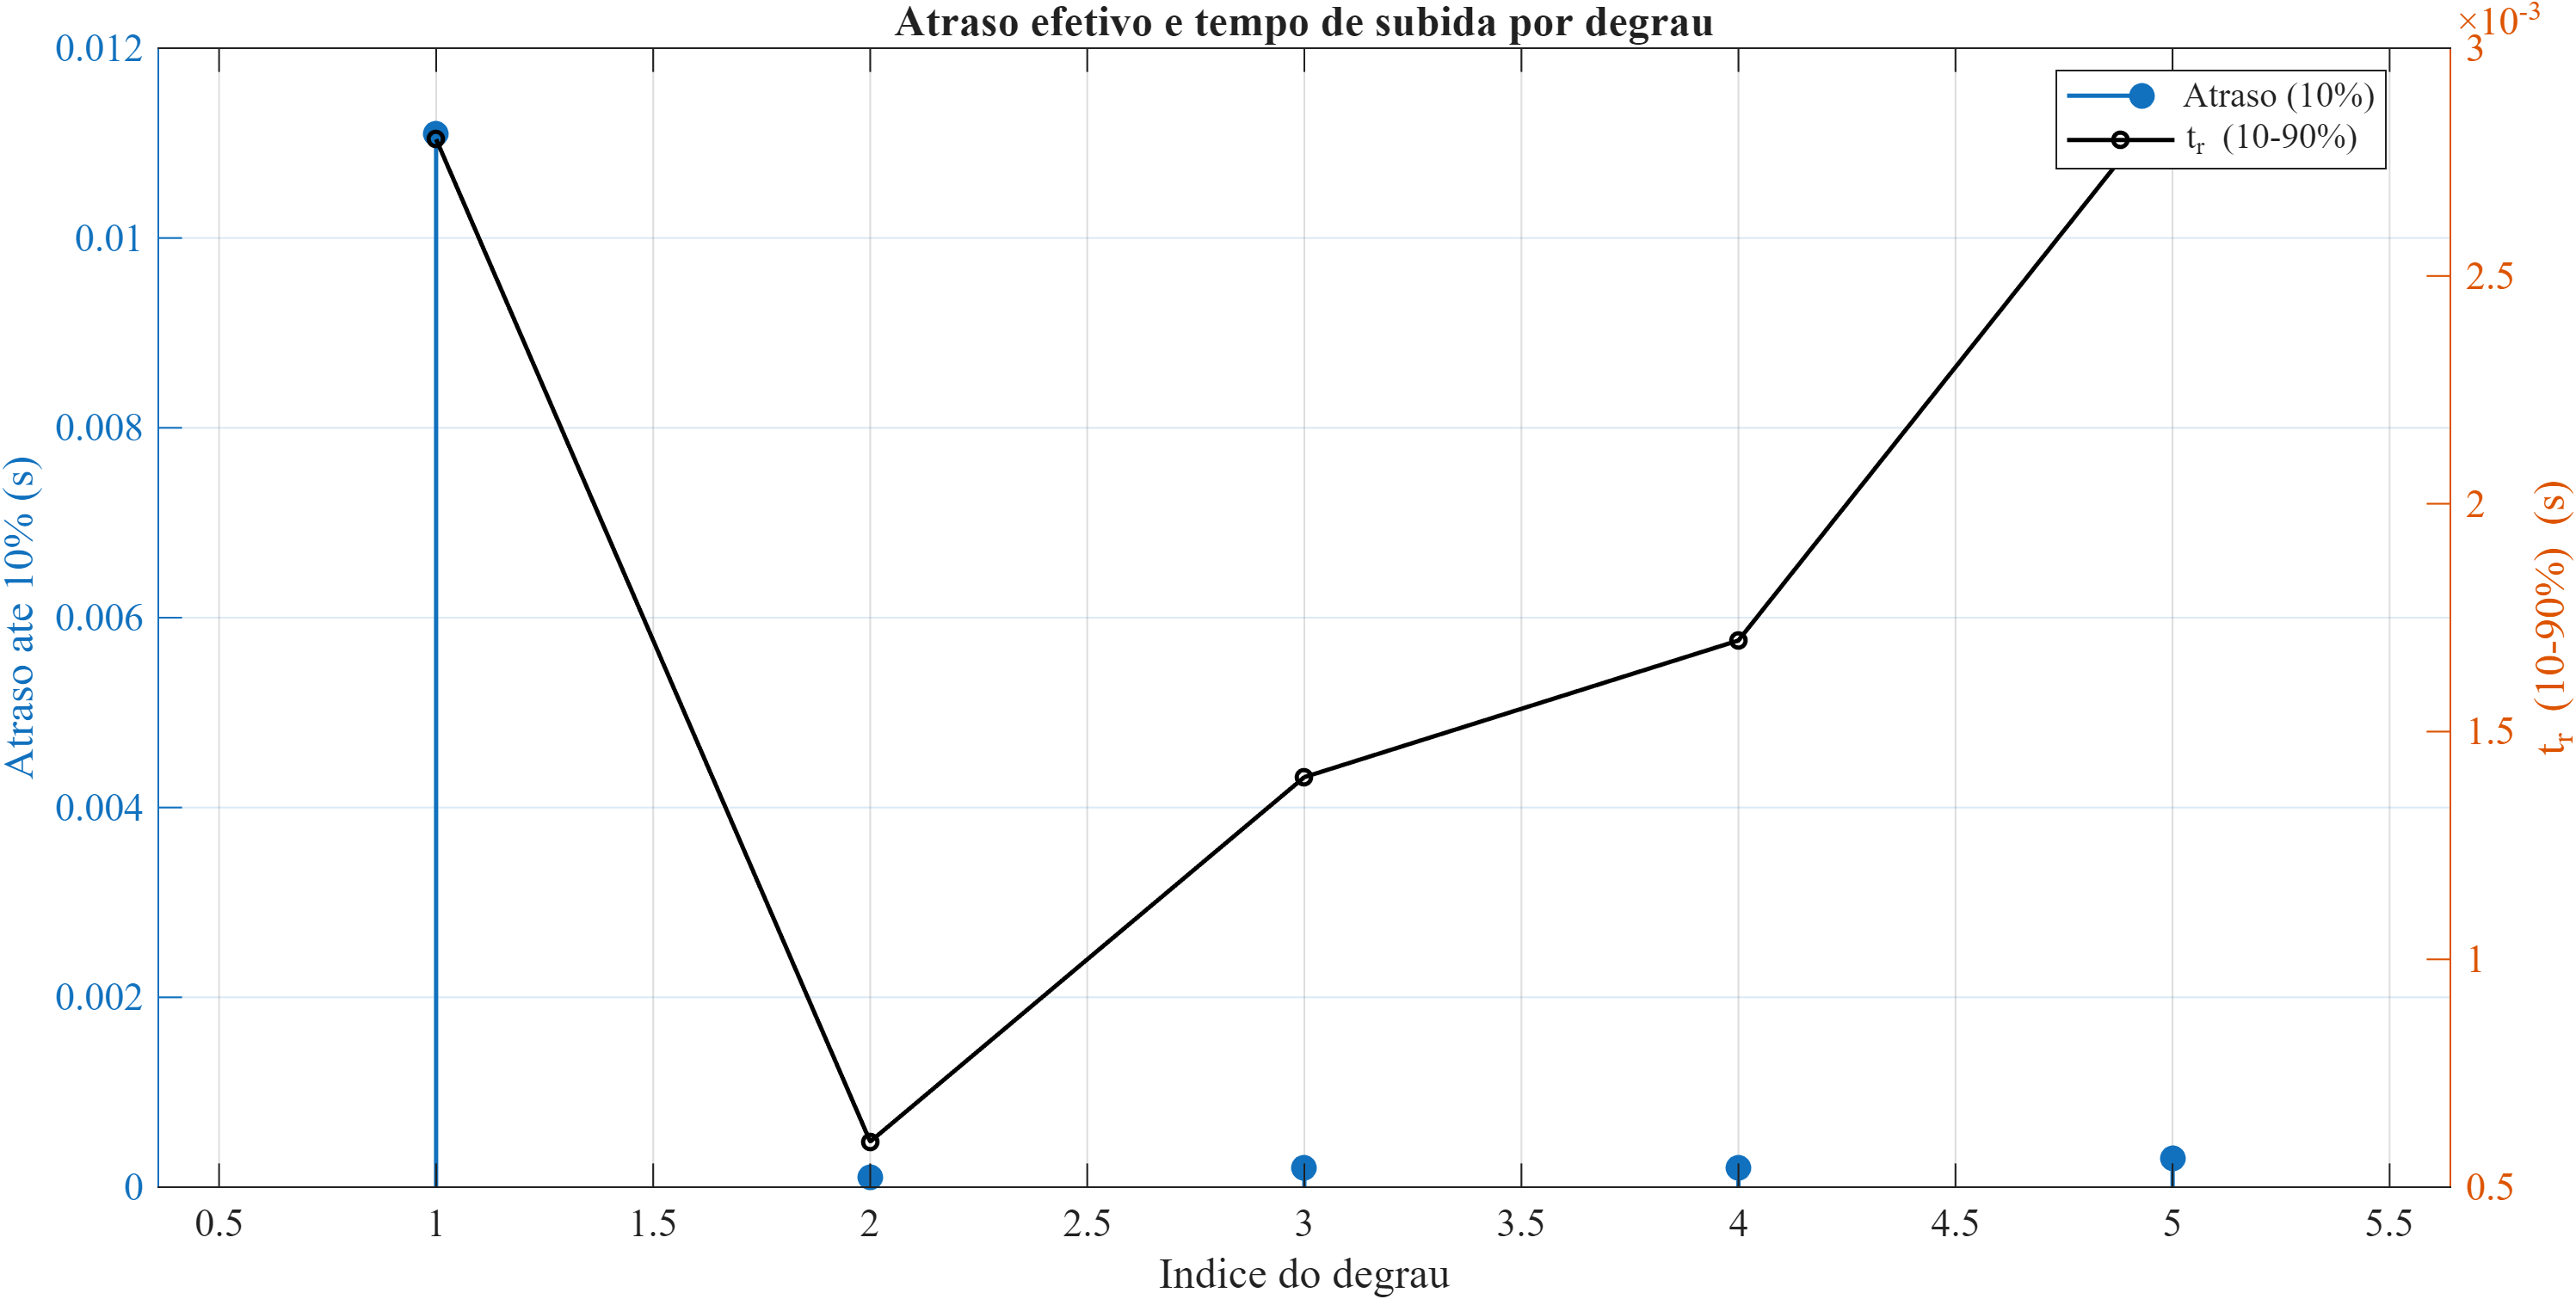
\includegraphics[width=8.4cm]{artigo_item07_atrasos_tempos.png}
         \caption{Atraso efetivo (até 10\%) e tempo de subida (10--90\%) estimados por degrau.}
         \label{fig:artigo_item07_atrasos_tempos}
      \end{center}
   \end{figure}

   A Figura~\ref{fig:artigo_item07_atrasos_tempos} organiza atrasos e tempos característicos por degrau, fornecendo uma visão compacta de ``largura de banda'' observada no canal de pressão. Esses indicadores são úteis para diferenciar limitações do atuador hidráulico de efeitos de discretização e de estimação em tempo discreto.
}{ }

\IfFileExists{artigo_item08_mapa_comando_pressao.png}{%
   \begin{figure}
      \begin{center}
         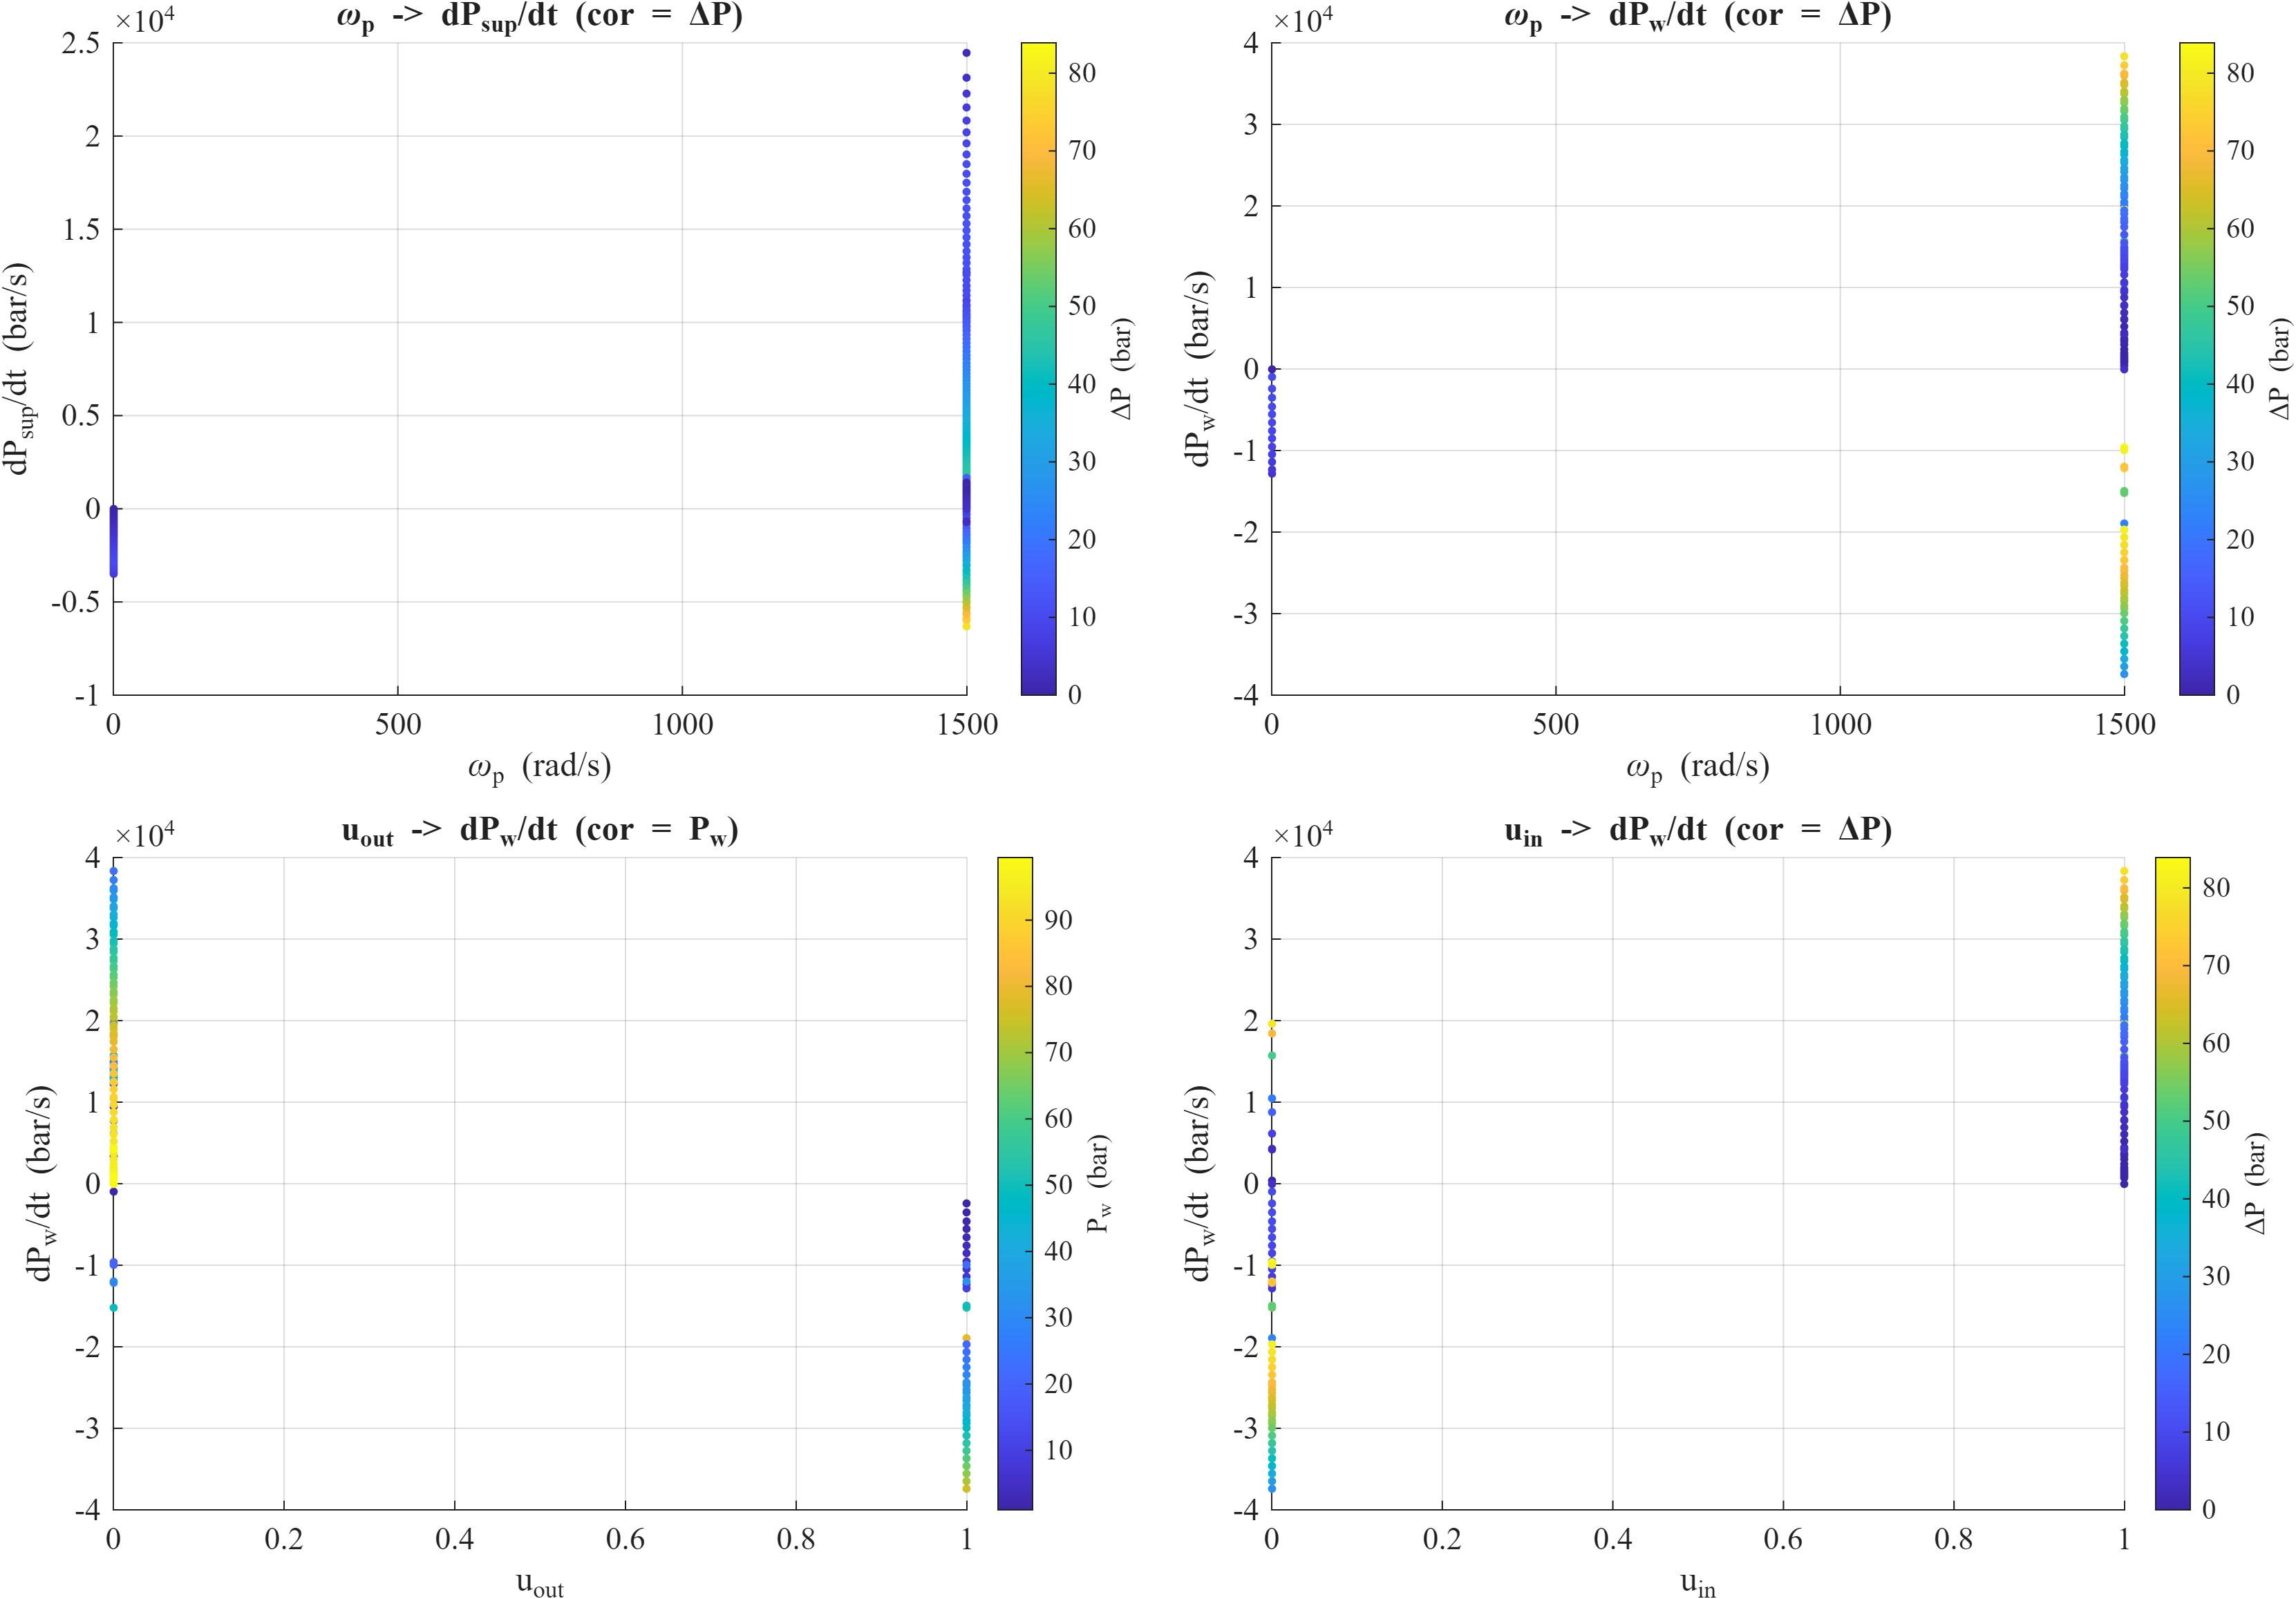
\includegraphics[width=8.4cm]{artigo_item08_mapa_comando_pressao.png}
         \caption{Mapas comando--efeito extraídos das séries temporais: relação entre comandos e taxas de variação de pressão.}
         \label{fig:artigo_item08_mapa_comando_pressao}
      \end{center}
   \end{figure}

   Para conectar diretamente a forma das curvas à modelagem, a Figura~\ref{fig:artigo_item08_mapa_comando_pressao} apresenta mapas entre comando e efeito hidráulico (por exemplo, comando versus $\mathrm{d}P/\mathrm{d}t$), evidenciando monotonicidade, regiões de ganho reduzido e influência do diferencial de pressão. Esse tipo de leitura é consistente com a interpretação física subjacente às leis de vazão baseadas em orifício \cite{ChenLv2017,Lv2014}.

   Os mapas de dispersão que relacionam comandos (velocidade da bomba e estados das válvulas) às taxas de variação de pressão ajudam a visualizar, de forma compacta, a não linearidade do sistema. A associação de $\omega_p$ a $\mathrm{d}P_{sup}/\mathrm{d}t$ e $\mathrm{d}P_w/\mathrm{d}t$, colorida por $\Delta P=P_{sup}-P_w$, evidencia que o ganho efetivo do canal de pressão depende fortemente da diferença de pressão disponível.

   De modo semelhante, os mapas envolvendo $u_{in}$ e $u_{out}$ mostram que a influência das válvulas na taxa de variação de $P_w$ é condicionada tanto pelo estado lógico (aberta/fechada) quanto pelo nível de pressão vigente. Esses resultados reforçam a interpretação de que o sistema apresenta comportamento fortemente não linear e dependente de regime, o que justifica o uso de uma abordagem baseada em simulação com modelo não linear para avaliação de desempenho, em vez de depender apenas de modelos lineares simplificados.
}{ }

\IfFileExists{artigo_item09_tradeoff_erro_esforco.png}{%
   \begin{figure}
      \begin{center}
         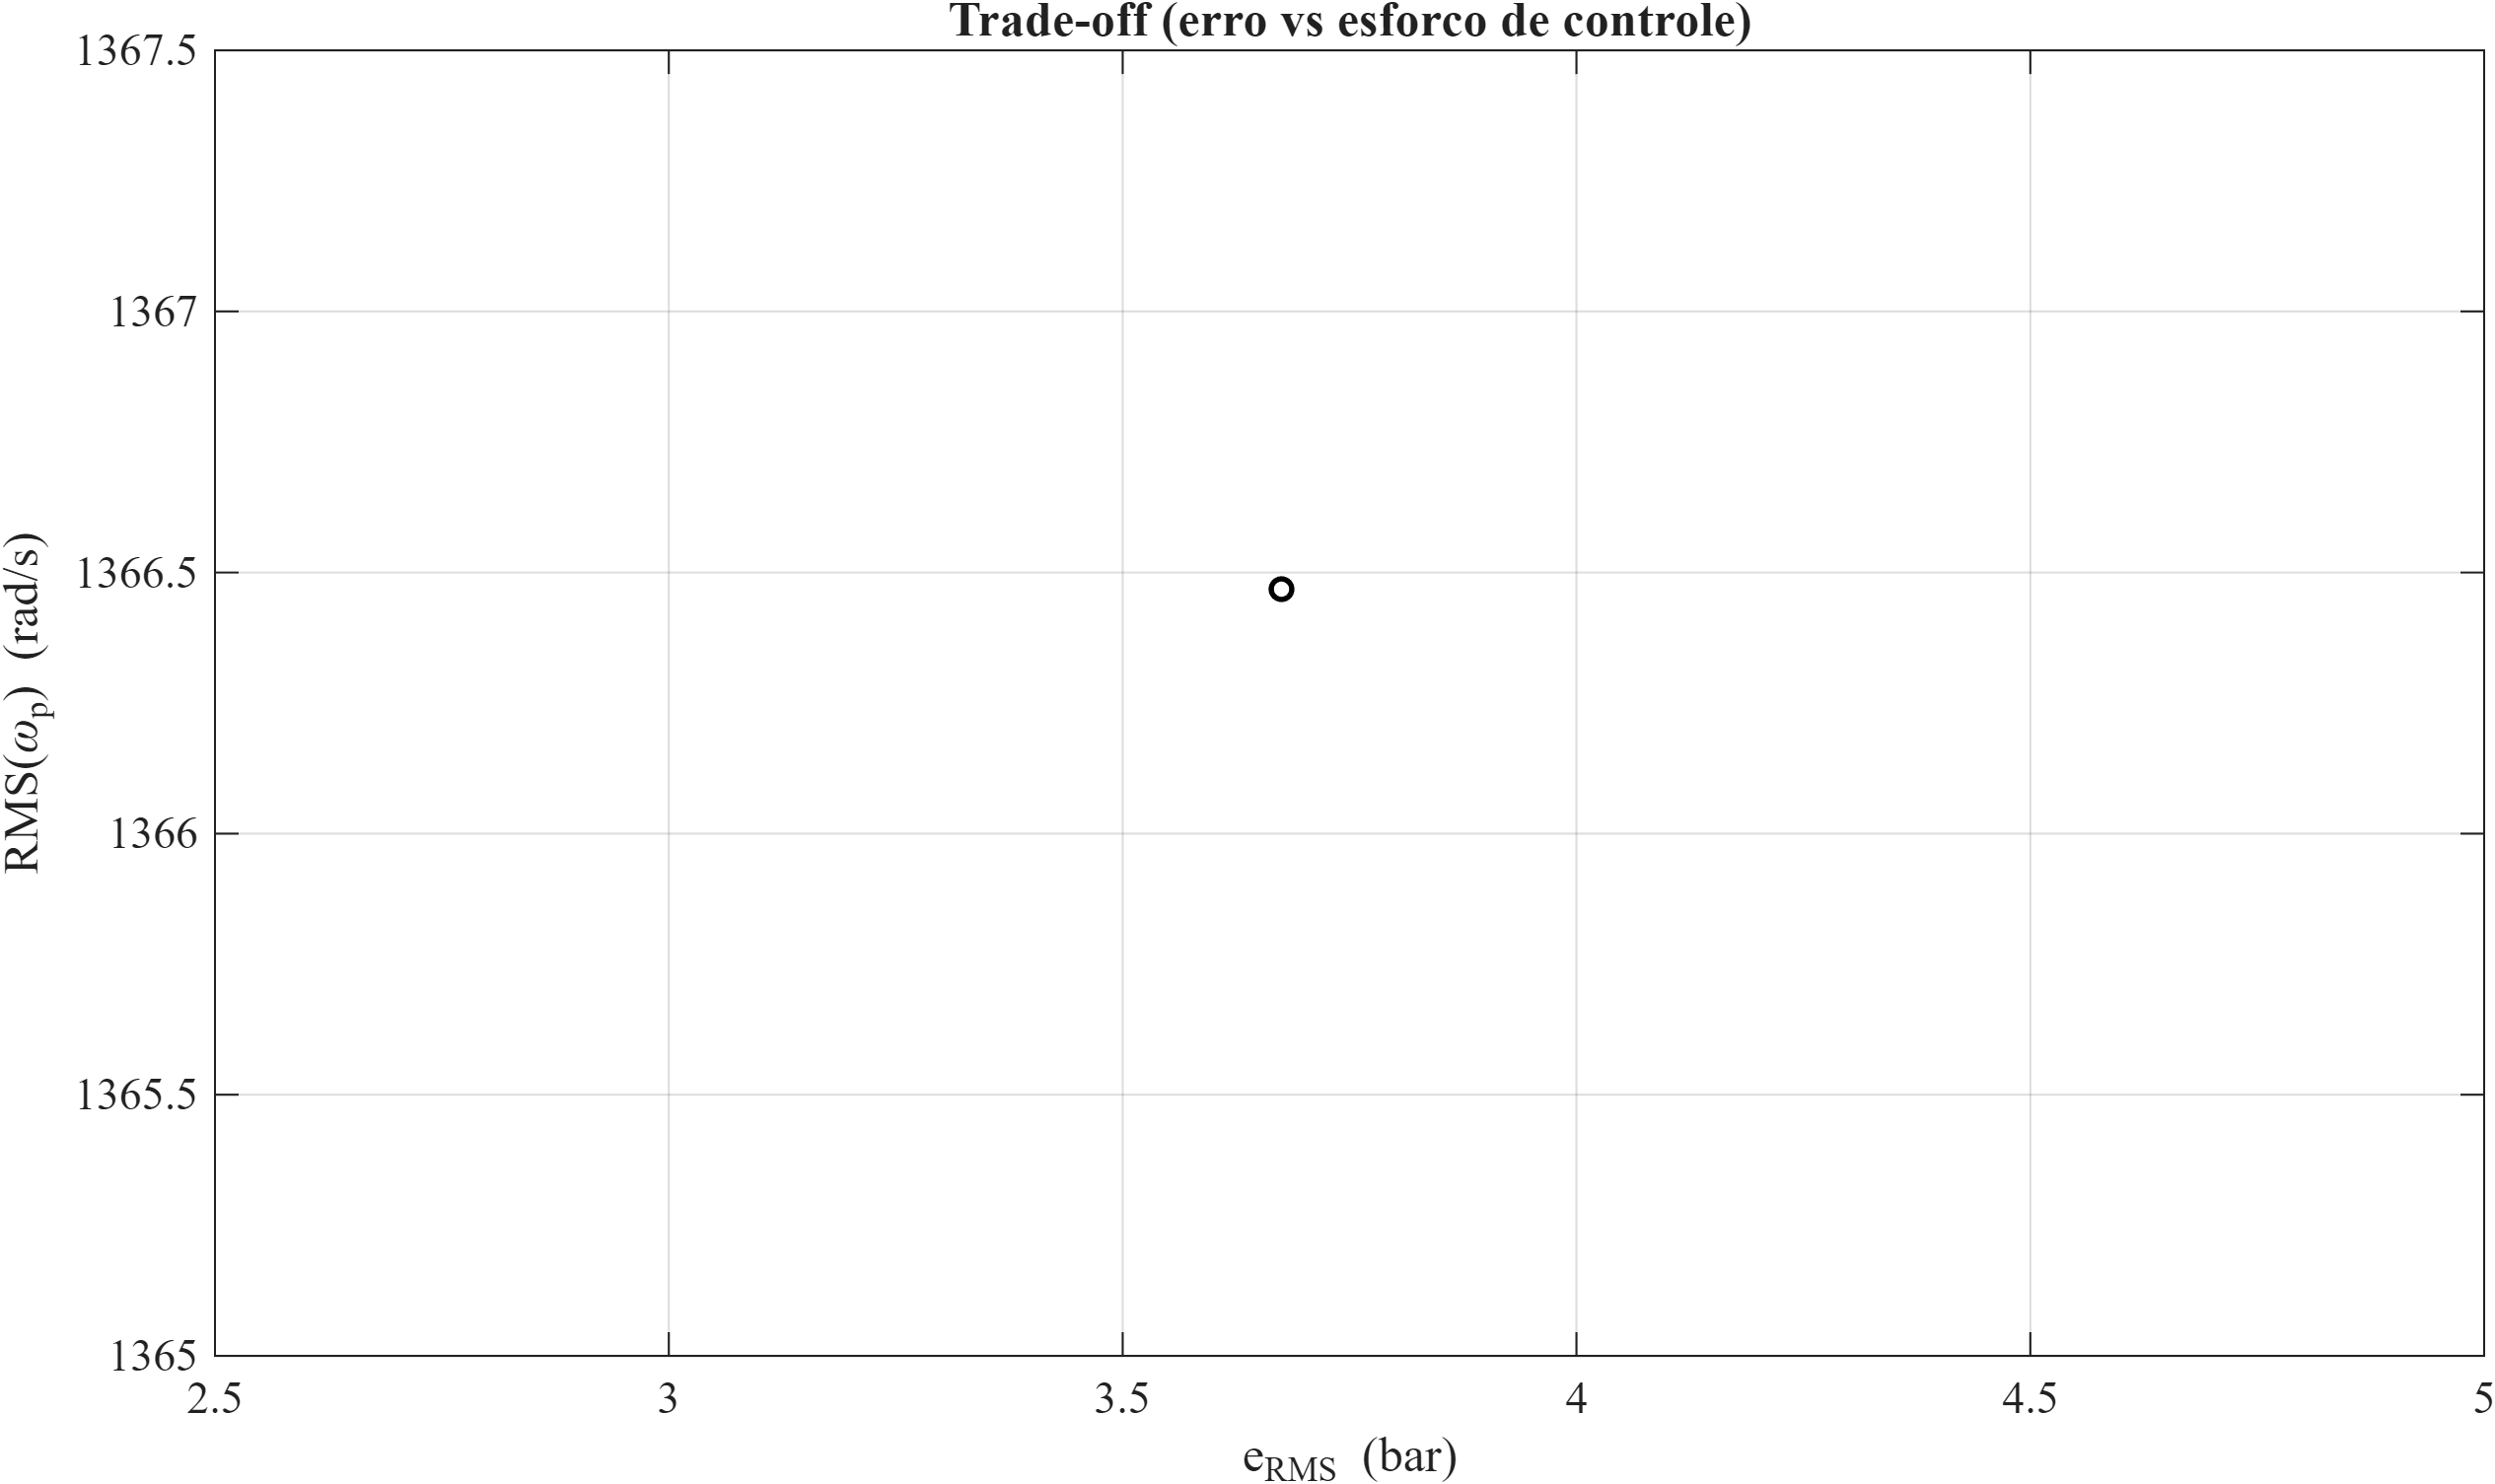
\includegraphics[width=8.4cm]{artigo_item09_tradeoff_erro_esforco.png}
         \caption{Trade-off entre erro de seguimento e esforço de controle (variação do peso em $R$).}
         \label{fig:artigo_item09_tradeoff_erro_esforco}
      \end{center}
   \end{figure}

   Para evitar conclusões dependentes de um único ajuste, a Figura~\ref{fig:artigo_item09_tradeoff_erro_esforco} explicita o compromisso entre erro e esforço de atuação associado a escolhas de ponderação do LQI. Essa apresentação é particularmente relevante em moduladores eletro-hidráulicos, nos quais reduzir erro pode elevar saturações, comutação e desgaste.
}{ }

\IfFileExists{artigo_item10_robustez_ruido.png}{%
   \begin{figure}
      \begin{center}
         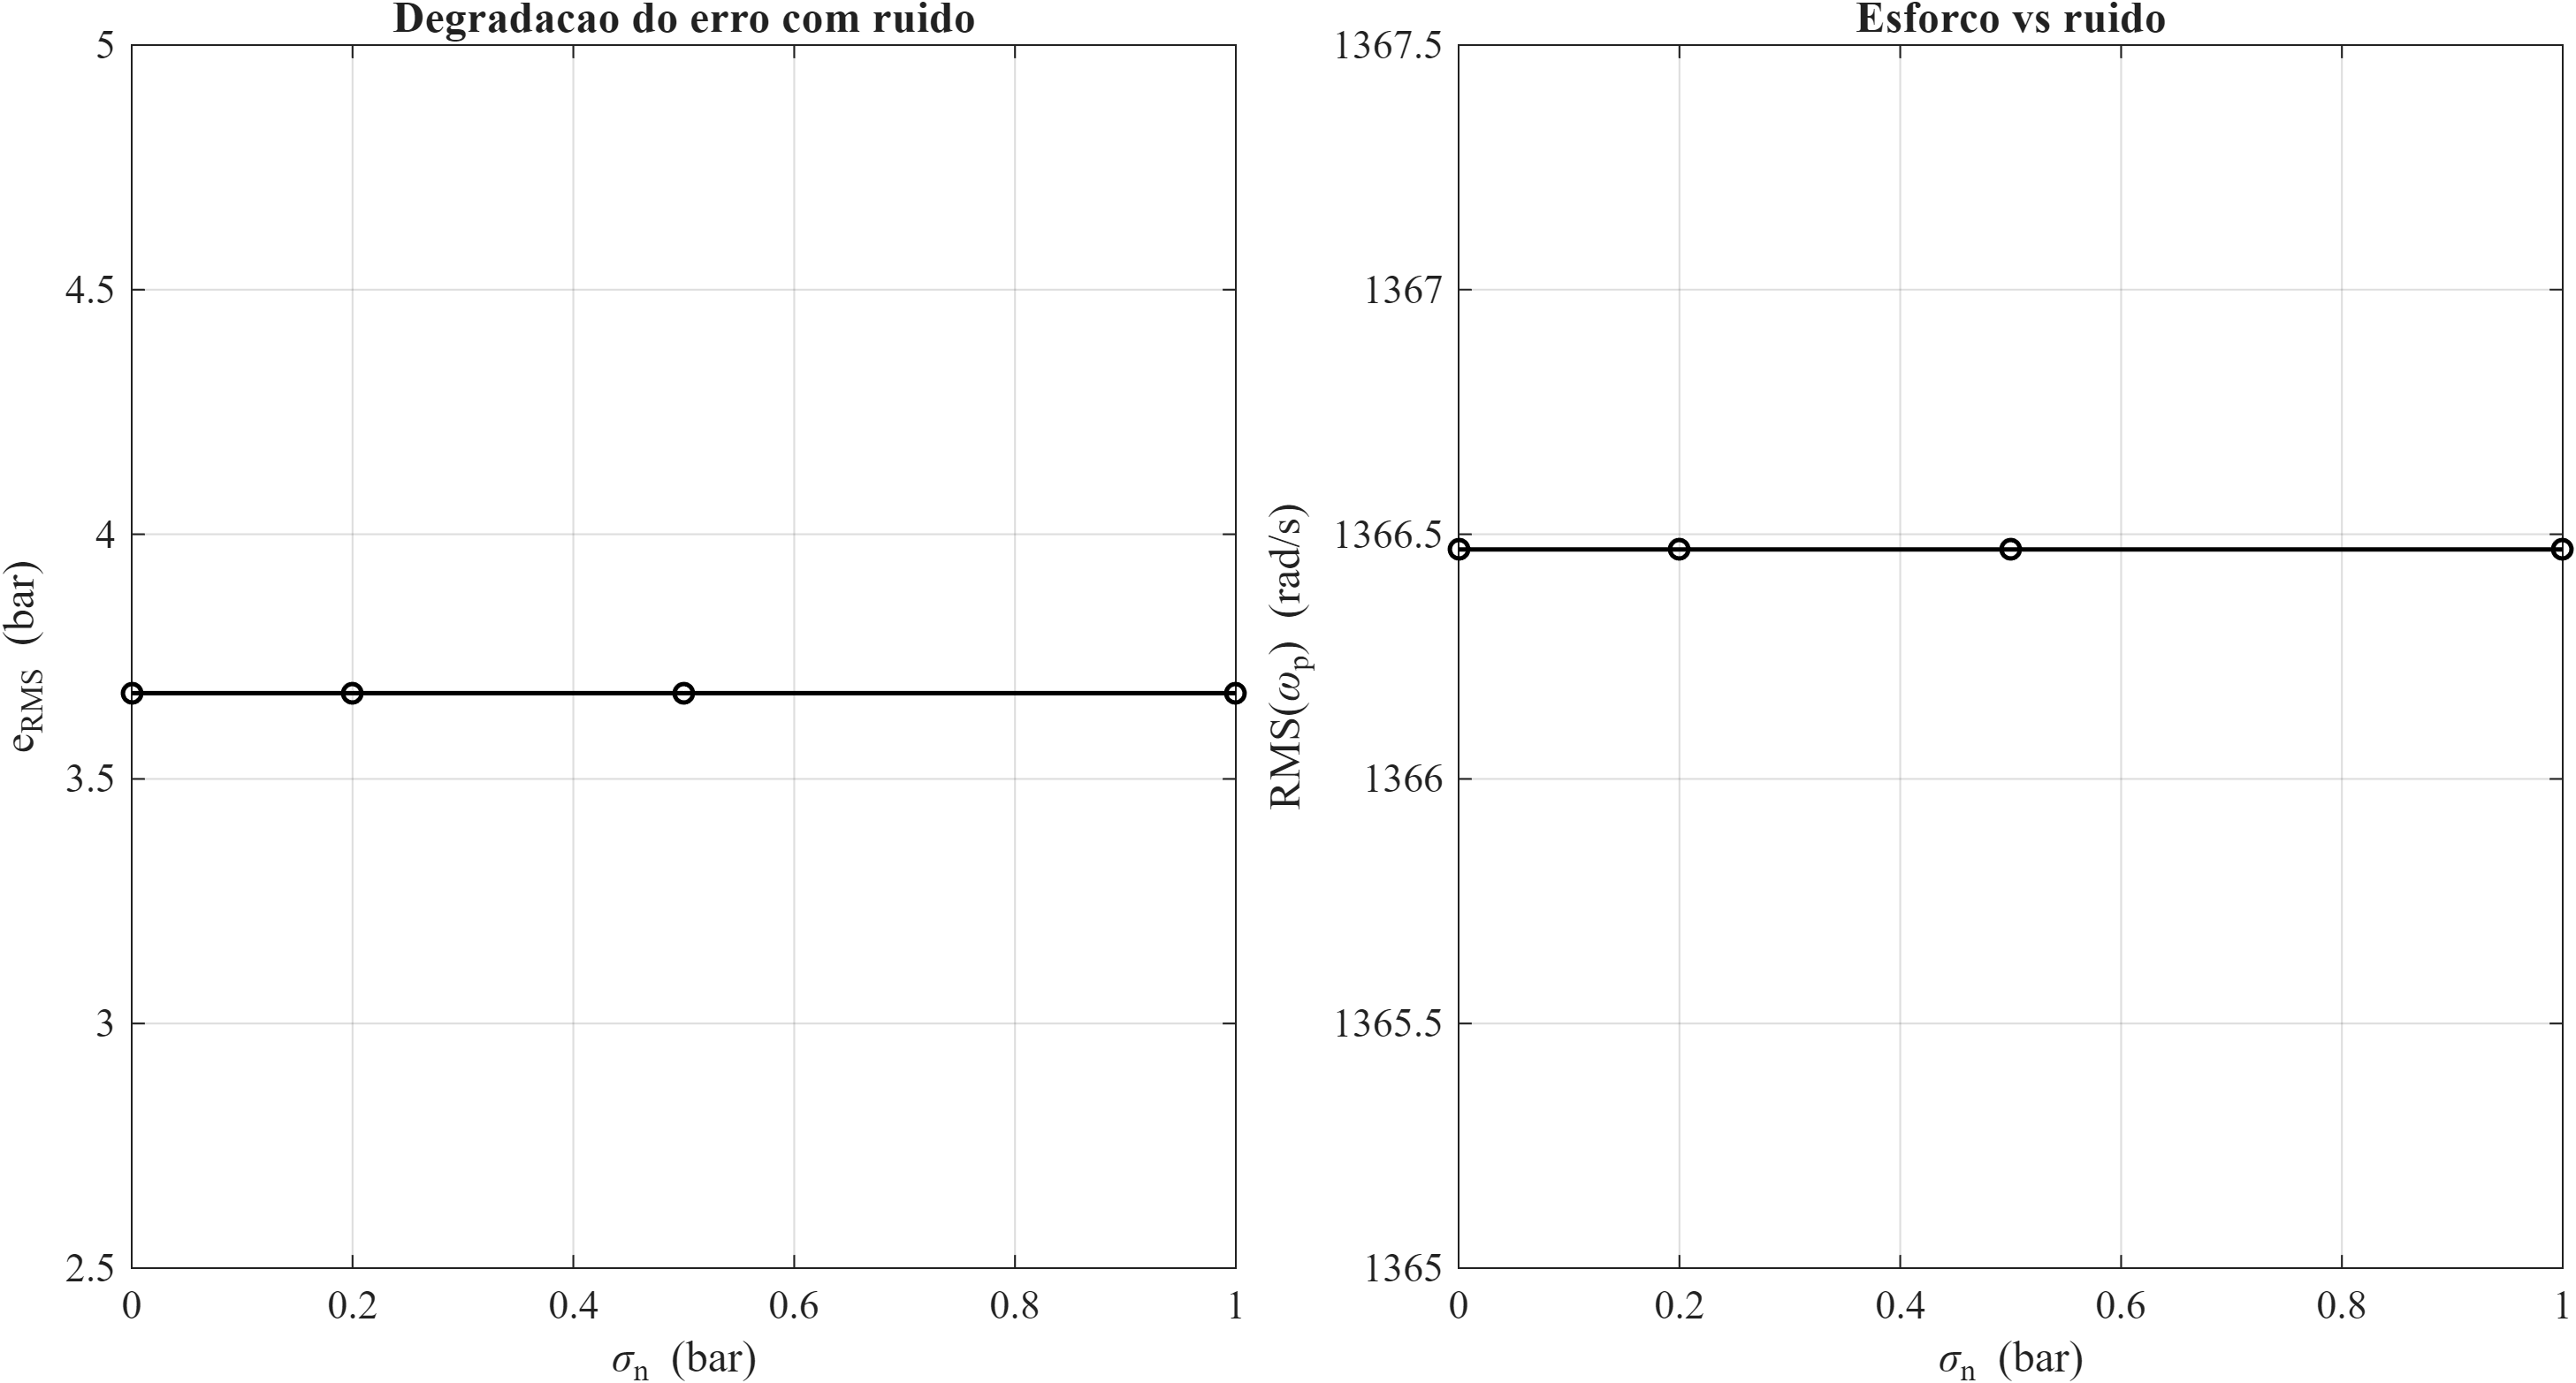
\includegraphics[width=8.4cm]{artigo_item10_robustez_ruido.png}
         \caption{Robustez a ruído de medição: degradação de métricas de erro e esforço em função do nível de ruído.}
         \label{fig:artigo_item10_robustez_ruido}
      \end{center}
   \end{figure}

   A Figura~\ref{fig:artigo_item10_robustez_ruido} resume o efeito do ruído de medição da pressão sobre as métricas globais de erro e esforço, complementando a Figura~\ref{fig:artigo_simulacao_ruido_medicao} com uma leitura agregada do impacto do ruído. À medida que o desvio padrão do ruído aumenta, observa-se um crescimento gradual do erro RMS e do esforço RMS do atuador, bem como um aumento na atividade de controle associada às correções sucessivas. No entanto, essa degradação é moderada na faixa de ruídos analisada (até 1~bar), sem indicar perda abrupta de desempenho.

   Esses resultados sugerem que o arranjo controlador--observador é capaz de tolerar níveis de ruído compatíveis com sensores reais de pressão, ainda que à custa de um aumento previsível na comutação e no desgaste dos atuadores. Do ponto de vista de projeto, isso indica que a escolha de sensores com qualidade razoável é suficiente para preservar o comportamento desejado, sem necessidade de requisitos excessivamente restritivos quanto a ruído.
}{ }

\IfFileExists{artigo_item11_transicoes_referencia.png}{%
   \begin{figure}
      \begin{center}
         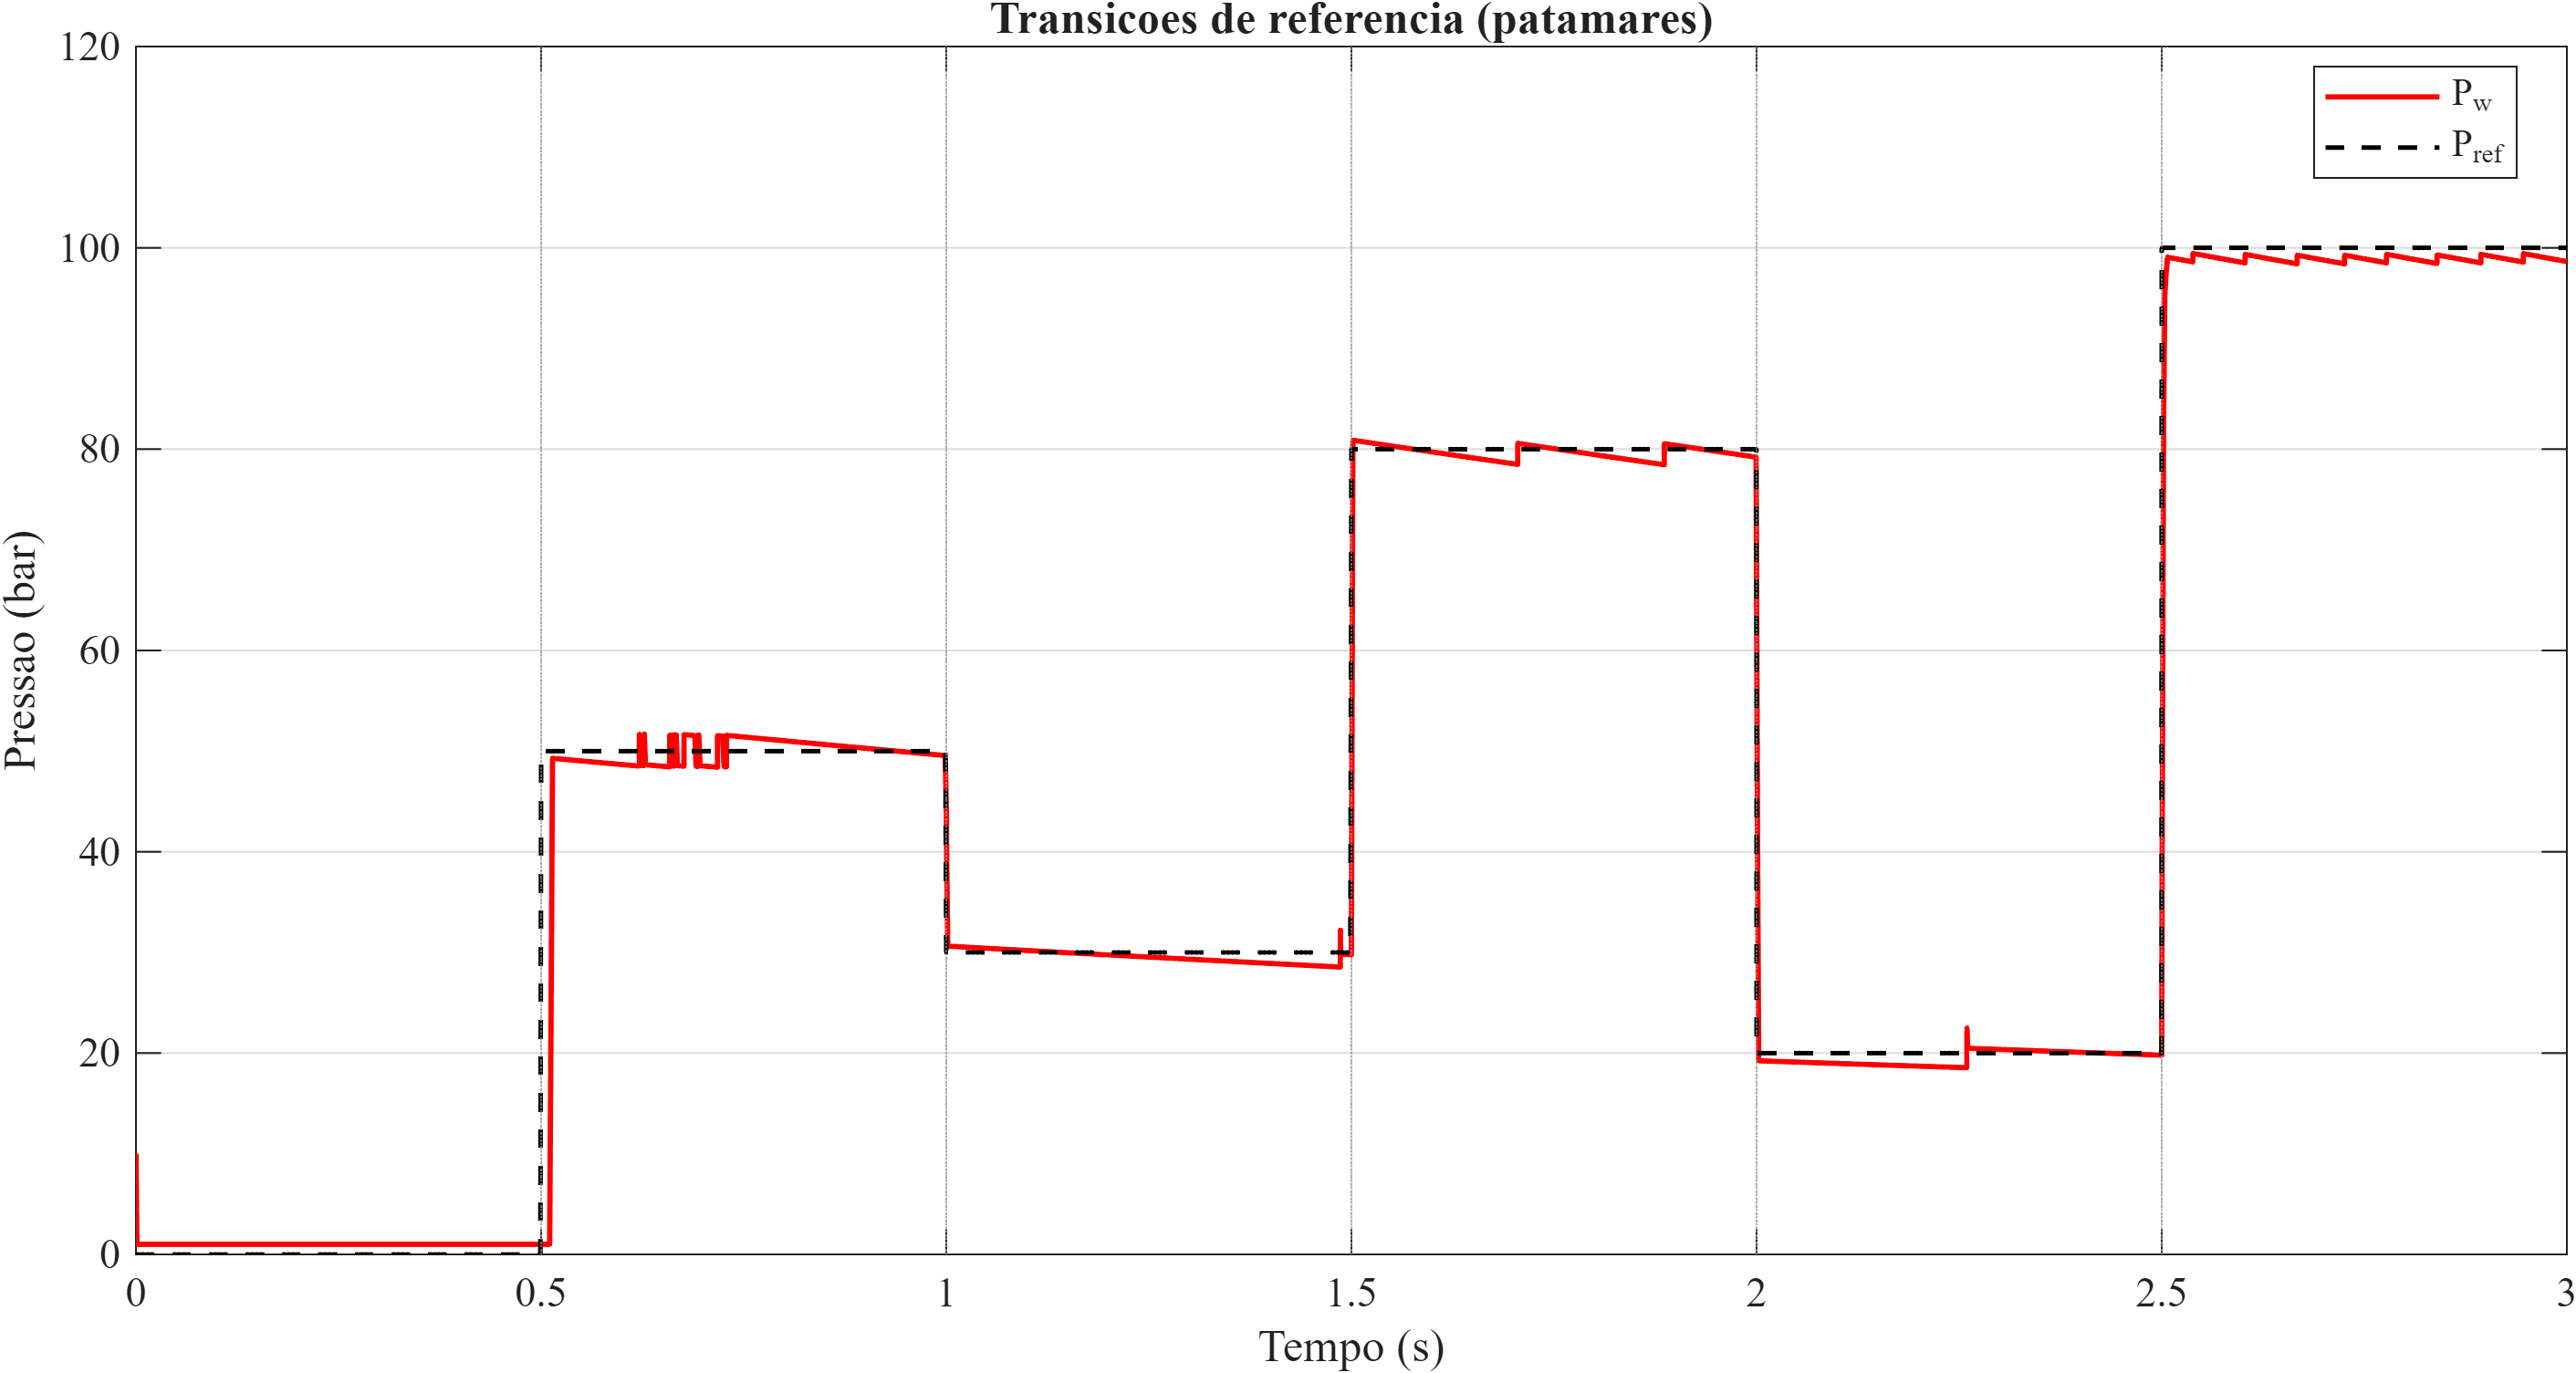
\includegraphics[width=8.4cm]{artigo_item11_transicoes_referencia.png}
         \caption{Transições de referência (patamares) destacadas no tempo, como cenário representativo de demanda externa.}
         \label{fig:artigo_item11_transicoes_referencia}
      \end{center}
   \end{figure}

   Embora o foco seja o regulador de baixa camada, as transições de patamar (Figura~\ref{fig:artigo_item11_transicoes_referencia}) representam mudanças de demanda compatíveis com integração a funções ADAS longitudinais, nas quais $P_{ref}$ é imposto por um controlador superior. A avaliação por segmentos permite discutir coerência do seguimento sob mudanças sucessivas de demanda, sem assumir um modelo completo de veículo.
}{ }

\IfFileExists{artigo_item12_plausibilidade_resumo.png}{%
   \begin{figure}
      \begin{center}
         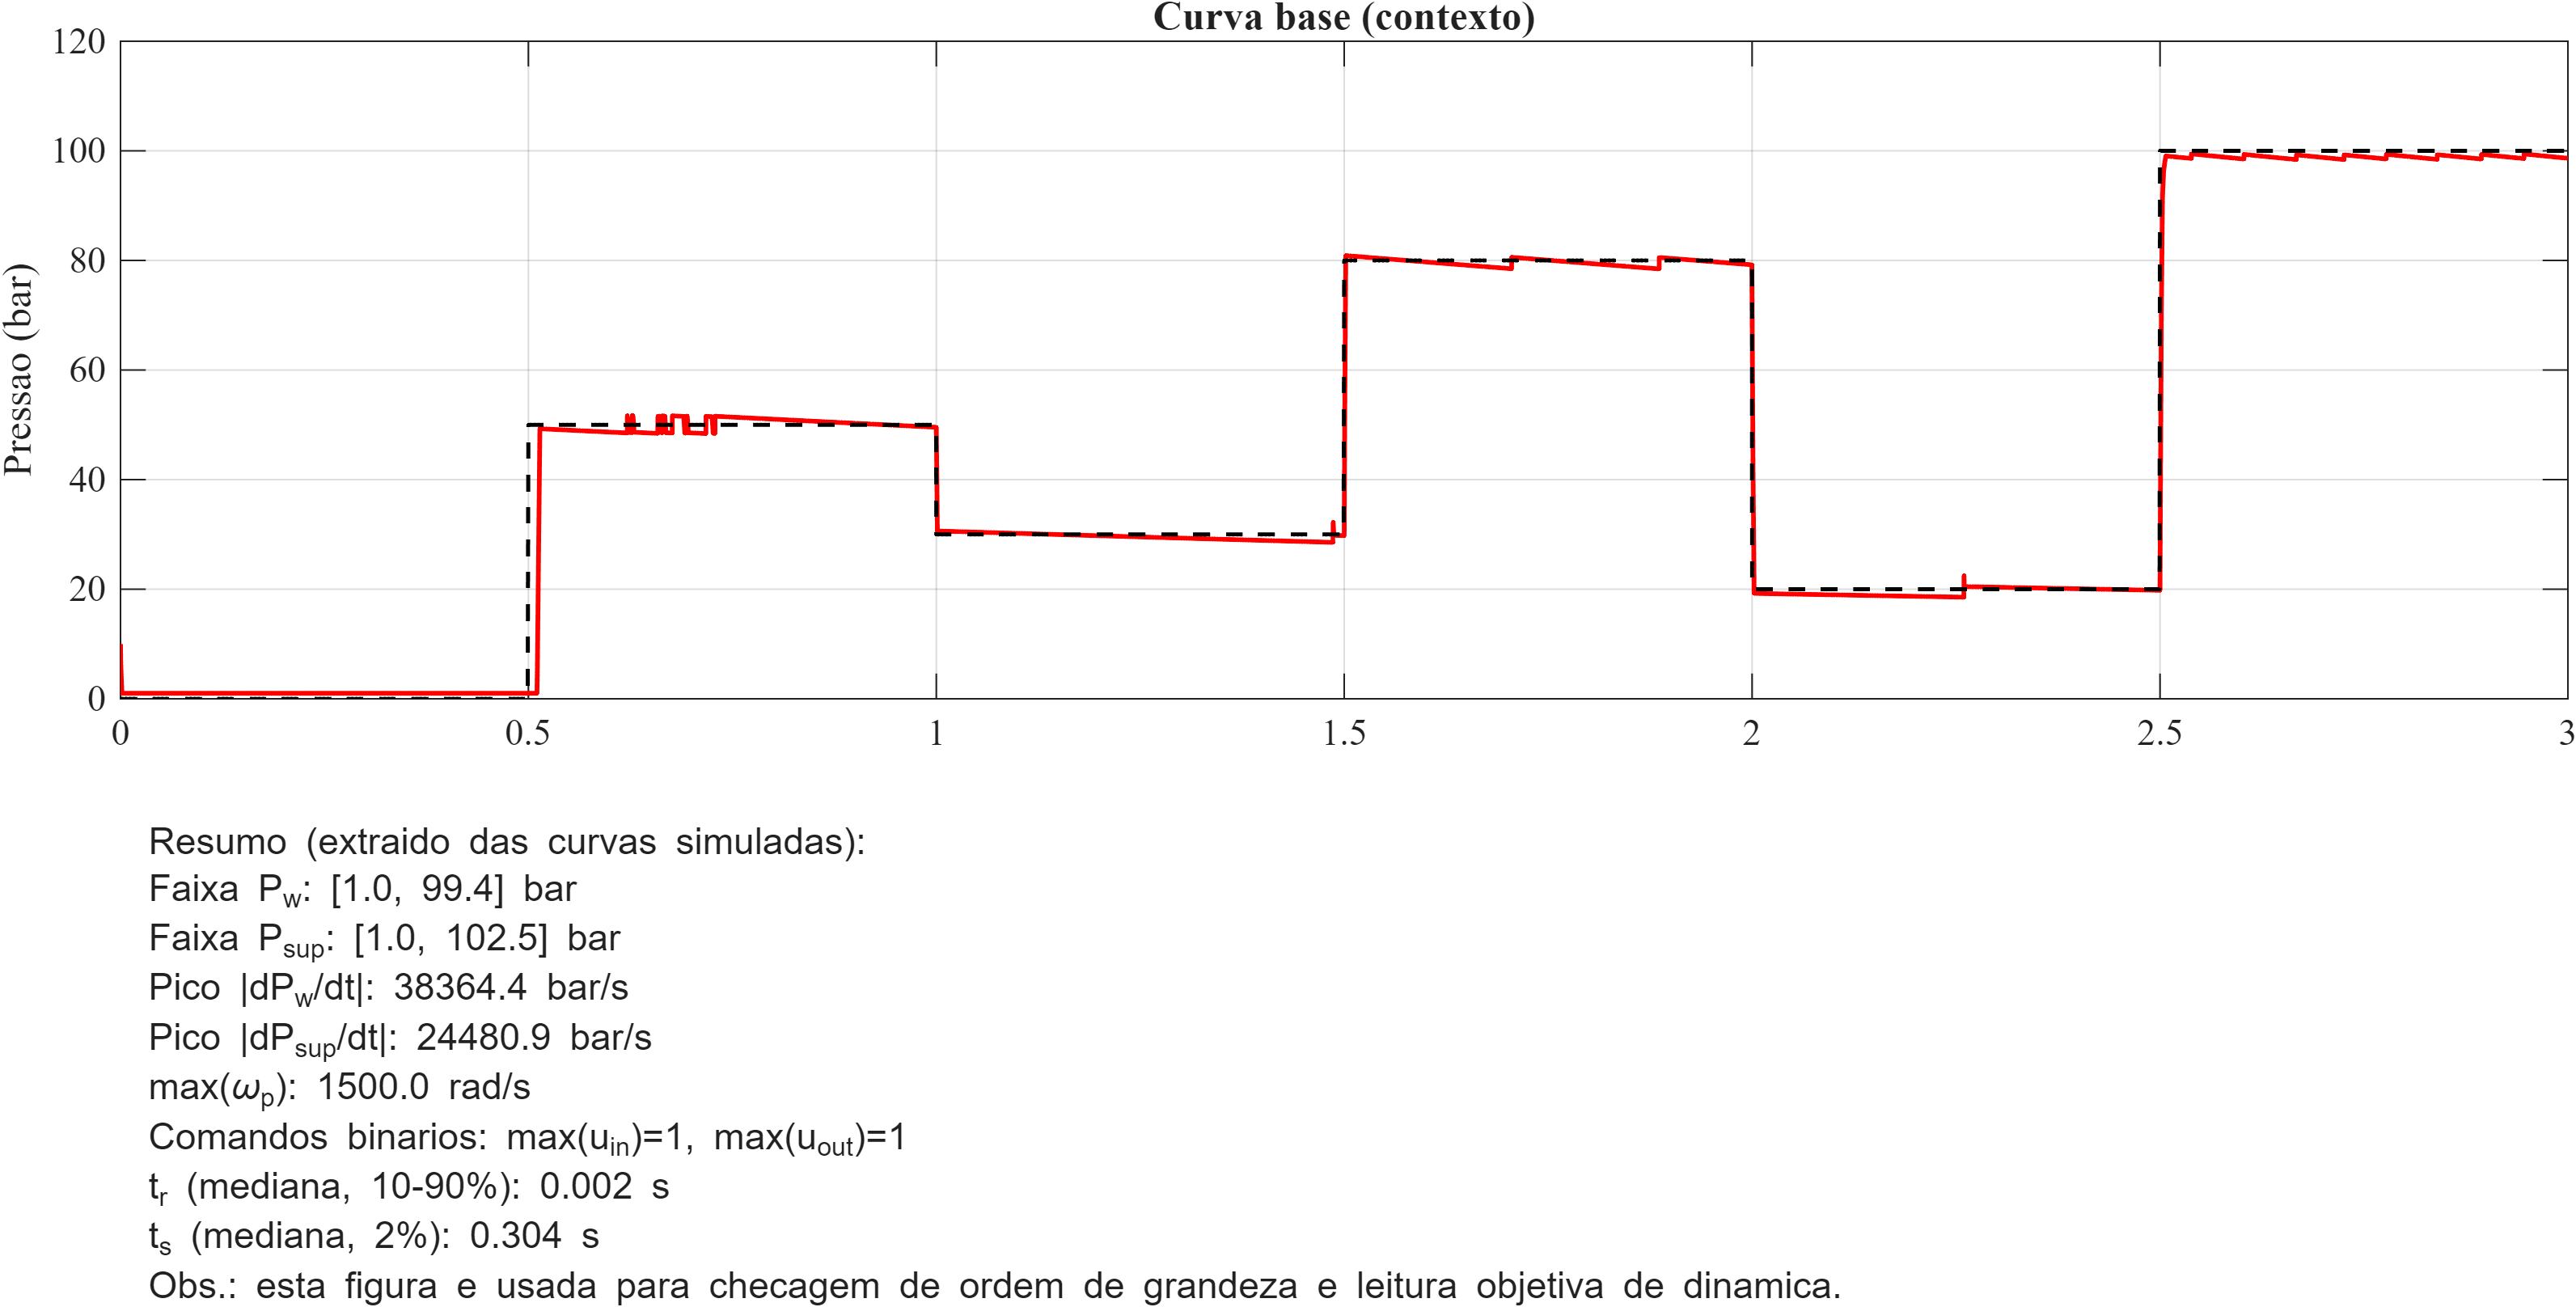
\includegraphics[width=8.4cm]{artigo_item12_plausibilidade_resumo.png}
         \caption{Resumo de ordens de grandeza extraídas das curvas simuladas (faixas, picos e tempos característicos).}
         \label{fig:artigo_item12_plausibilidade_resumo}
      \end{center}
   \end{figure}

   A Figura~\ref{fig:artigo_item12_plausibilidade_resumo} consolida, em um único painel, a curva base de referência e as principais ordens de grandeza extraídas das simulações. As faixas de pressão observadas em $P_w$ e $P_{sup}$, os picos de $\left|\mathrm{d}P/\mathrm{d}t\right|$, os limites de $\omega_p$ e os tempos típicos de subida e acomodação são compatíveis com o que se espera para moduladores hidráulicos empregados em sistemas de freio automotivos.

   A consistência dessas ordens de grandeza com tendências reportadas na literatura e com especificações usuais de sistemas ABS/ESC reforça a plausibilidade física do modelo utilizado \cite{HouhuaJing2022,ZengYangHuang2023,Lv2014,ChenLv2017}. Assim, além de servir como ferramenta de projeto e avaliação de controle, o modelo concentrado adotado mostra-se aderente ao comportamento qualitativo e quantitativo de moduladores reais, o que é um requisito importante para a relevância prática dos resultados apresentados.
}{ }

\IfFileExists{artigo_extra_discretizacao.png}{%
   \begin{figure}
      \begin{center}
         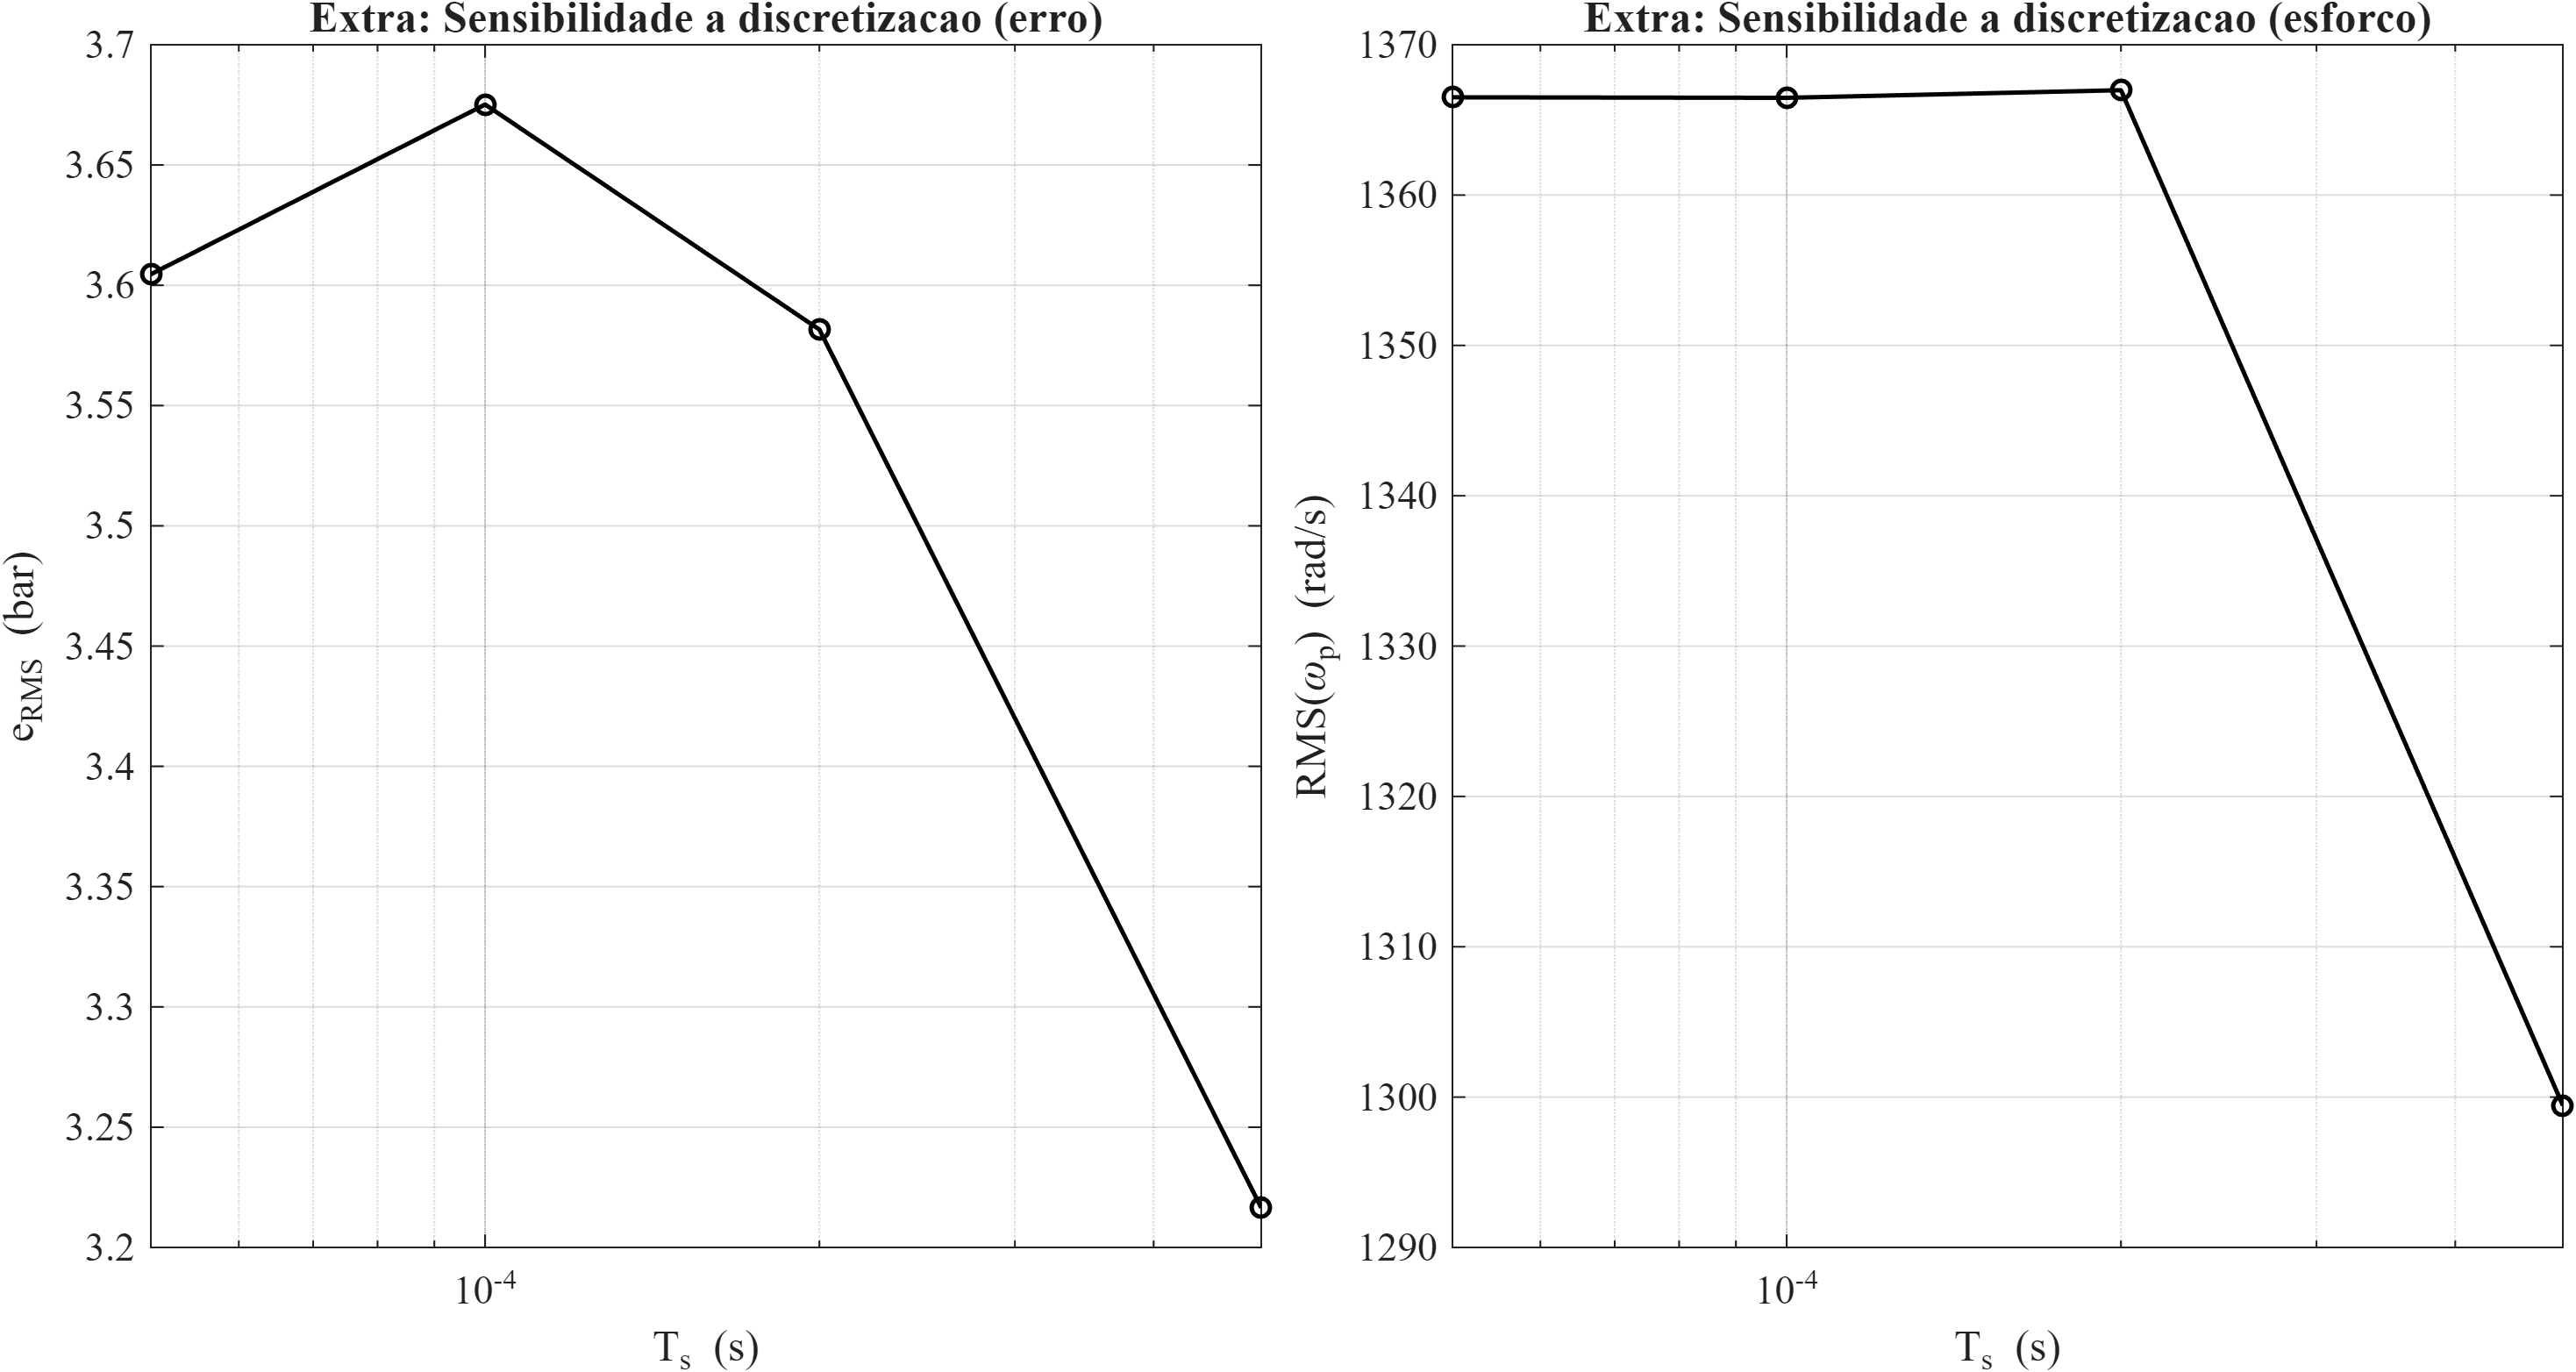
\includegraphics[width=8.4cm]{artigo_extra_discretizacao.png}
         \caption{Robustez à discretização: sensibilidade de métricas ao período de amostragem $T_s$.}
         \label{fig:artigo_extra_discretizacao}
      \end{center}
   \end{figure}

   Em aplicações embarcadas, a escolha de $T_s$ influencia simultaneamente desempenho, esforço e robustez do observador. Assim, a Figura~\ref{fig:artigo_extra_discretizacao} é usada para discutir a sensibilidade do desempenho à discretização e separar limitações do atuador hidráulico de artefatos numéricos associados ao laço digital.
}{ }

\IfFileExists{artigo_simulacao_ruido_medicao.png}{%
   \begin{figure}
      \begin{center}
         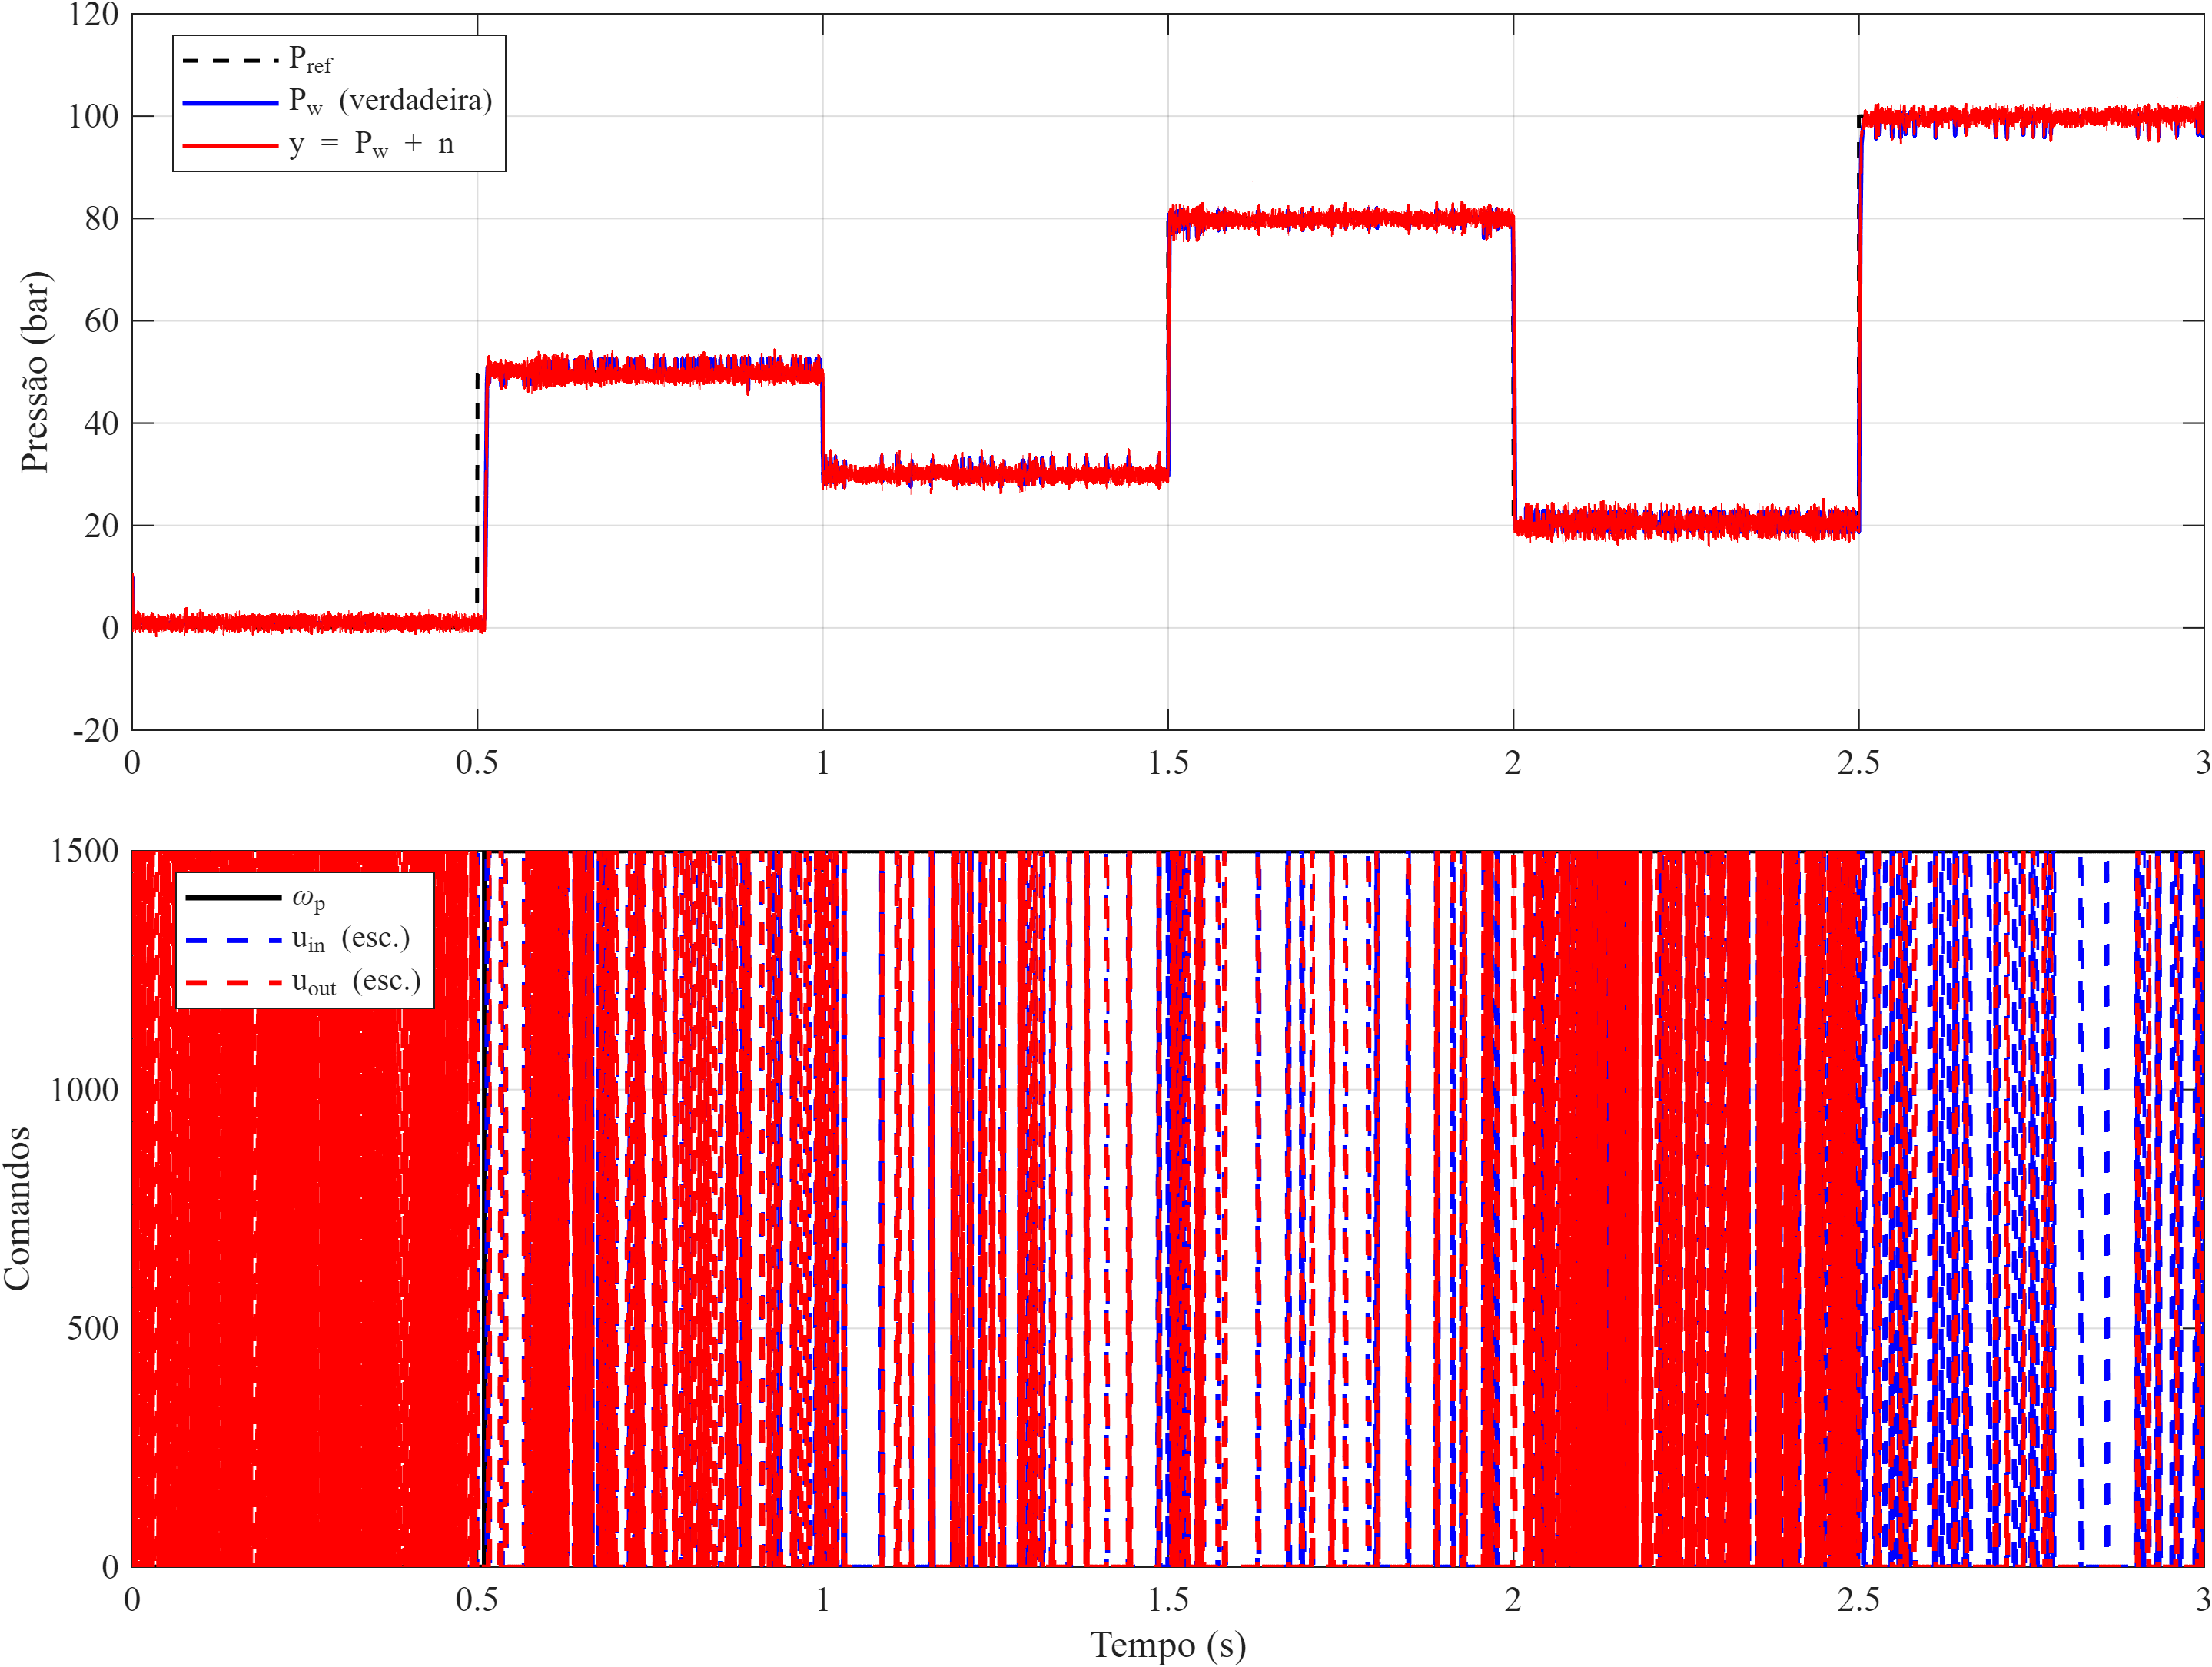
\includegraphics[width=8.4cm]{artigo_simulacao_ruido_medicao.png}    % The printed column width is 8.4 cm.
         \caption{Ensaio em malha fechada com ruído de medição em $P_w$ (sinal usado pelo observador).}
         \label{fig:artigo_simulacao_ruido_medicao}
      \end{center}
   \end{figure}

   O ensaio com ruído de medição (Figura~\ref{fig:artigo_simulacao_ruido_medicao}) explora a sensibilidade do observador e da lógica de válvulas a perturbações na variável medida. O interesse é caracterizar, de forma objetiva, como incertezas na medição de $P_w$ se refletem no compromisso entre flutuações do sinal usado pelo observador e comutação excessiva de válvulas, aspecto frequentemente crítico em sistemas eletro-hidráulicos.

   A Figura~\ref{fig:artigo_simulacao_ruido_medicao} ilustra, no domínio do tempo, o impacto do ruído de medição sobre a trajetória de seguimento. Mesmo com a presença de ruído na medida de pressão utilizada pelo observador, o seguidor continua acompanhando os patamares de referência, com erros em regime que permanecem em faixas reduzidas. O principal efeito visível é o aumento do \textit{ripple} em torno de cada patamar e a presença de pequenas flutuações no erro de seguimento.

   Em conjunto com os resultados agregados da Figura~\ref{fig:artigo_item10_robustez_ruido}, essa visualização reforça a interpretação de que o ruído de medição degrada o desempenho de forma gradual e controlada, sem comprometer a estabilidade da malha ou a capacidade de rastreamento dos patamares de referência. Do ponto de vista da aplicação em sistemas ABS/ESC, isso é relevante, pois sinaliza que o controlador proposto é compatível com níveis de ruído plausíveis em sensores de pressão automotivos.
}{}

Em síntese, os resultados desta seção estabelecem (i) coerência causal e ordem de grandeza do modelo não linear em malha aberta e (ii) viabilidade de seguimento de referência em malha fechada sob restrições de atuação e lógica discreta. Esses achados delimitam o que o modelo e o regulador demonstram no escopo de simulação e motivam, como passos seguintes, a consolidação de métricas sumarizadas e a exploração sistemática de sensibilidade paramétrica quando o objetivo for comparar configurações e hipóteses de modelagem.

\section{Conclusões}
\label{sec:conclusoes}
Este artigo apresentou um fluxo metodológico para projeto e avaliação, em simulação, de um regulador digital de pressão hidráulica por roda usando o módulo ABS/ESC como atuador em frenagem ativa. A combinação de modelo não linear concentrado, linearização local, síntese LQI em tempo discreto, observador de Luenberger e lógica discreta de válvulas fornece uma arquitetura compatível com restrições de atuação e com requisitos típicos de integração a funções ADAS longitudinais \cite{Lentin2022,Konrad2014}.

Os resultados devem ser interpretados dentro do escopo proposto: evidência em ambiente MATLAB/Simulink, voltada à coerência do controle e à compatibilidade com restrições de atuação e instrumentação. As simulações em malha aberta e em malha fechada organizam um conjunto mínimo de evidências para sustentar a modelagem adotada e a pertinência de combinar regulador em tempo discreto, observador e lógica de válvulas no contexto de frenagem ativa.

A seção de resultados inclui um conjunto de análises diretamente extraídas das curvas simuladas: métricas por degrau, envelopes de $\mathrm{d}P/\mathrm{d}t$ e saturações, assimetria entre pressurização e alívio, avaliação de ondulação em regime, checagem local de consistência entre modelo linearizado e planta não linear, varreduras paramétricas focadas e estudo do compromisso erro--esforço. Além disso, inclui-se uma avaliação de sensibilidade ao período de amostragem para discutir robustez da implementação discreta.

Como limitações, o estudo não pretende representar um veículo completo (dinâmica longitudinal/pneu) nem substituir validação experimental do atuador; além disso, a síntese é baseada em linearização local e a atuação de válvulas é representada por lógica binária com histerese. Como continuidade natural, destacam-se a implementação embarcada do regulador em microcontrolador automotivo, a verificação de temporização do laço de controle, o tratamento de efeitos de quantização/ruído e a validação em bancada/HIL com instrumentação mínima de pressão, de modo a consolidar a transferência do \textit{model-in-the-loop} para o ambiente físico \cite{KapinskiJamesDeshmukh2016}.

\bibliography{ifacconf}             % bib file to produce the bibliography
% with bibtex (preferred)

%\begin{thebibliography}{xx}  % you can also add the bibliography by hand

%\bibitem[Able(1956)]{Abl:56}
%B.C. Able.
%\newblock Nucleic acid content of microscope.
%\newblock \emph{Nature}, 135:\penalty0 7--9, 1956.

%\bibitem[Able et~al.(1954)Able, Tagg, and Rush]{AbTaRu:54}
%B.C. Able, R.A. Tagg, and M.~Rush.
%\newblock Enzyme-catalyzed cellular transanimations.
%\newblock In A.F. Round, editor, \emph{Advances in Enzymology}, volume~2, pages
%  125--247. Academic Press, New York, 3rd edition, 1954.

%\bibitem[Keohane(1958)]{Keo:58}
%R.~Keohane.
%\newblock \emph{Power and Interdependence: World Politics in Transitions}.
%\newblock Little, Brown \& Co., Boston, 1958.

%\bibitem[Powers(1985)]{Pow:85}
%T.~Powers.
%\newblock Is there a way out?
%\newblock \emph{Harpers}, pages 35--47, June 1985.

%\bibitem[Soukhanov(1992)]{Heritage:92}
%A.~H. Soukhanov, editor.
%\newblock \emph{{The American Heritage. Dictionary of the American Language}}.
%\newblock Houghton Mifflin Company, 1992.

%\end{thebibliography}
\end{document}
